\begin{savequote}[75mm]
At its heart, engineering is about using science to find creative, practical solutions. It is a noble profession.
\qauthor{--- Queen Elizabeth II ---}
\end{savequote}

\chapter{Polar coordinates and parametric equations}
\label{chap_parametric}
\graphicspath{{figures/Parametric/}}


\section{Polar coordinates}
\label{sec_polar}
\subsection{Definition}
In Section~\ref{CartesianPlane}, we introduced the Cartesian coordinates of a point in the plane as a means of assigning ordered pairs of numbers to points in the plane.  We defined the Cartesian coordinate plane using two number lines -- one horizontal and one vertical -- which intersect at right angles at a point we called the origin. For this reason, the Cartesian coordinates of a point are often called \index{rectangular coordinates}\index{coordinates ! rectangular}\textbf{rectangular coordinates} (\textit{rechthoekige co\"ordinaten}) \index[aut]{rechthoekige co\"ordinaten}. In this section, we introduce a new system for assigning coordinates to points in the plane --  \index{polar coordinates}\index[aut]{poolco\"ordinaten}\textbf{polar coordinates} (\textit{poolco\"ordinaten}).  We start with an origin point, called the \index{polar coordinates ! pole}\index[aut]{poolco\"ordinaten ! pool}\textbf{pole} (\textit{pool}), and a ray called the \index{polar coordinates ! polar axis}\index[aut]{poolco\"ordinaten ! poolas}\textbf{polar axis} (\textit{poolas}). We then locate a point $P$ using two coordinates, $(r,\theta)$, where $r$ represents a directed distance from the pole and $\theta$ is a measure of rotation from the polar axis (Figure~\ref{fig_parametric_1}).  Roughly speaking,  the polar coordinates $(r,\theta)$ of a point measure how far out the point is from the pole (that is $r$), and how far to rotate from the polar axis, (that is $\theta$).


\begin{figure}
	\begin{center}
			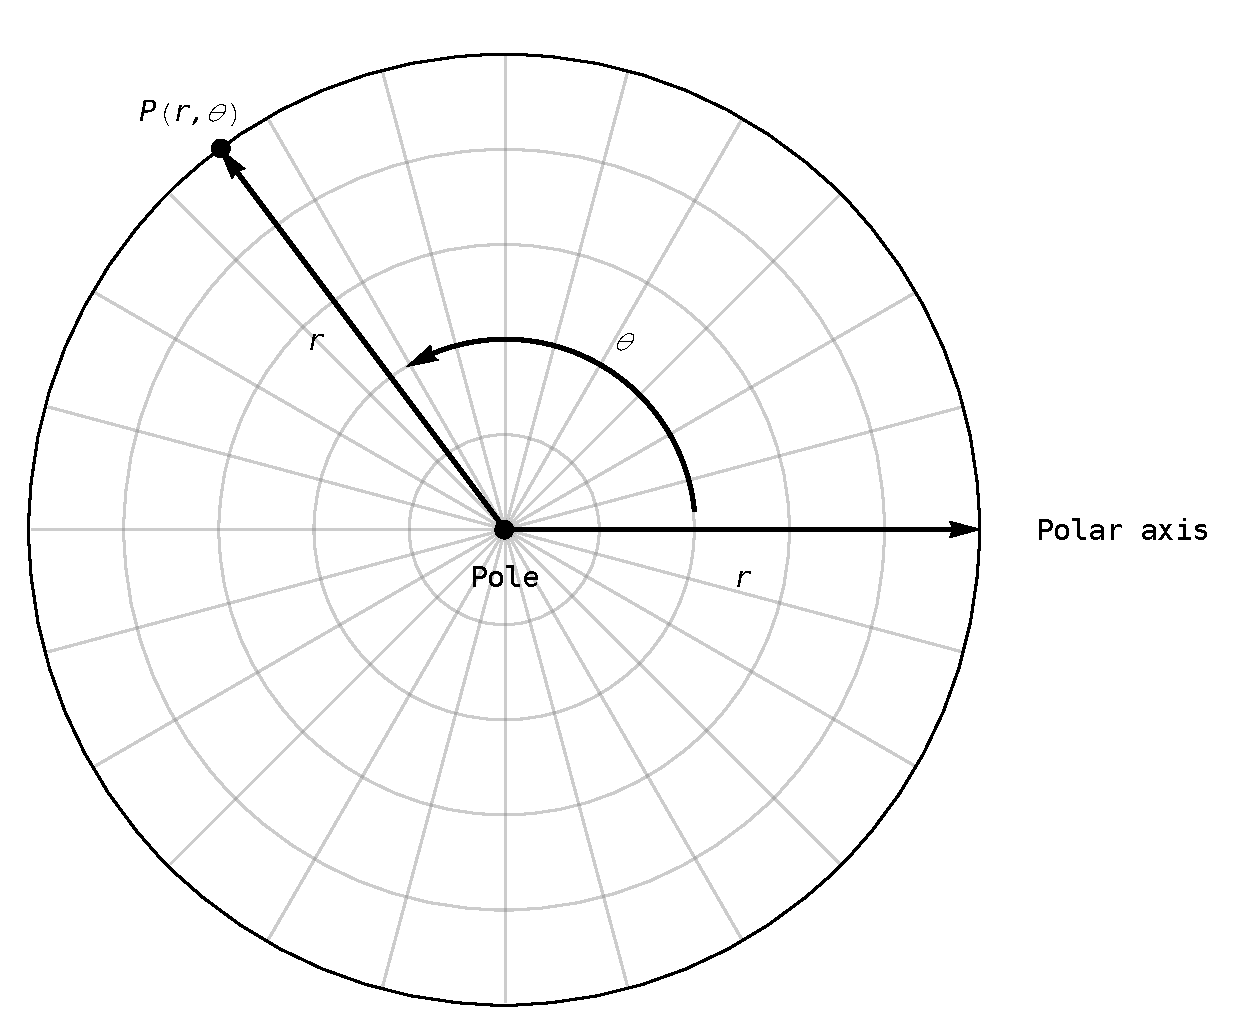
\includegraphics[width=0.5\textwidth]{fig_parametric_1}
	\caption{Polar coordinate system. }
	\label{fig_parametric_1}
	\end{center}
\end{figure}

For example, if we wish to plot the point $P$ with polar coordinates $\left(4, \frac{5\pi}{6}\right)$, we would start at the pole, move out along the polar axis $4$ units, then rotate $\frac{5\pi}{6}$ radians counter-clockwise. We may also consider this process by thinking of the rotation first. To plot $P\left(4,\frac{5\pi}{6}\right)$ this way,  we rotate  $\frac{5\pi}{6}$ counter-clockwise from the polar axis, then move outwards from the pole $4$ units.  

If $r < 0$, we begin by moving in the opposite direction on the polar axis from the pole and as you may have guessed, $\theta < 0$ means the rotation away from the polar axis is clockwise instead of counter-clockwise. Furthermore, it should come as no surprise that any given point expressed in polar coordinates has infinitely many other representations in polar coordinates.  More formally, suppose $\left(r, \theta\right)$ and $\left(\widetilde{r}, \widetilde{\theta}\right)$ are polar coordinates where $r \neq 0$, $\widetilde{r} \neq 0$ and the angles are measured in radians.  Then $\left(r, \theta\right)$ and $\left(\widetilde{r}, \widetilde{\theta}\right)$  determine the same point $P$ if and only if one of the following is true:
 
 \begin{itemize}
 
 \item  $\widetilde{r} = r$ and $\widetilde{\theta} =  \theta + 2\pi k$ for some integer $k$,
 
 \item  $\widetilde{r} = -r$ and $\widetilde{\theta} =  \theta + (2k + 1) \pi$ for some integer $k$.
 
 \end{itemize}

Moreover, all polar coordinates of the form $(0, \theta)$ represent the pole regardless of the value of $\theta$.

\begin{remark}[Polar coordinates in aviation]
Aircraft use a slightly modified version of the polar coordinates for navigation. In this system, the one generally used for any sort of navigation, the zero-degree ray is generally called heading 360, and the angles continue in a clockwise direction, rather than counterclockwise, as in the mathematical system. Heading 360 corresponds to magnetic north, while headings 90, 180, and 270 correspond to magnetic east, south, and west, respectively. Thus, an aircraft traveling 5 nautical miles due east will be traveling 5 units at heading 90.
\end{remark}


\subsection{Linking polar and rectangular coordinates}
To marry the polar coordinate system with the Cartesian (rectangular) coordinate system we identify the pole and polar axis in the polar system with the origin and positive $x$-axis, respectively, in the rectangular system.  We get the following result.



\begin{theorem}[Conversion between rectangular and polar coordinates] \label{polarrectangularconversion} 
Suppose a point $P$ is represented in rectangular coordinates as $(x,y)$ and in polar coordinates as $(r,\theta)$.  Then

\begin{itemize}

\item $x = r \cos(\theta)$ and $y = r\sin(\theta)\,;$ 

\item $x^2+y^2 = r^2$ and $\tan(\theta) = \dfrac{y}{x}$ (provided $x \neq 0$)\,. 

\end{itemize}

\end{theorem}


In the case $r > 0$, Theorem~\ref{polarrectangularconversion} is an immediate consequence of Theorem~\ref{cosinesinecircle} along with the definition of the tangent. If $r < 0$, then we know an alternate representation for $(r,\theta)$ is $(-r, \theta + \pi)$. Since we have that  $\cos(\theta+\pi) = -\cos(\theta)$ and $\sin(\theta + \pi) = -\sin(\theta)$, applying the theorem to $(-r,\theta+\pi)$ gives 
$$
\left\{\begin{array}{rcl}
x &=& (-r) \cos(\theta + \pi) = (-r)(-\cos(\theta)) = r\cos(\theta)\\[0.2cm]
y& =& (-r) \sin(\theta + \pi) = (-r)(-\sin(\theta)) = r\sin(\theta).
\end{array}
\right.
$$
Moreover, $x^2 + y^2 = (-r)^2 = r^2$, and $\frac{y}{x} = \tan(\theta + \pi) = \tan(\theta)$, so the theorem is true in this case, too.  The remaining case is $r = 0$, in which case $(r,\theta) = (0,\theta)$ is the pole.  Since the pole is identified with the origin $(0,0)$ in rectangular coordinates, the theorem in this case amounts to checking $0=0$.  The following example puts Theorem~\ref{polarrectangularconversion} to good use.

\begin{example}  \label{pointconversionex}  
 Convert each point in rectangular coordinates given below into polar coordinates with $r \geq 0$ and $0 \leq \theta < 2\pi$. 

\begin{multicols}{2}

\begin{enumerate}

\item  $P\left(2,-2\sqrt{3}\right)$


\item  $R(0,-3)$


\end{enumerate}

\end{multicols}

\xhrulefill{gray}{2.5pt}Solution \xhrulefill{gray}{2.5pt}


\begin{enumerate}

\item  The point $P\left(2,-2\sqrt{3}\right)$ lies in Quadrant IV.  With $x = 2$ and $y = -2\sqrt{3}$, we get 
$$r^2 = x^2 + y^2 = (2)^2 + \left(-2\sqrt{3}\right)^2 = 4+12 = 16\,,$$ 
so $r = \pm 4$.  Since we are asked for $r \geq 0$, we choose $r = 4$.  To find $\theta$, we have that 
$$\tan(\theta) = \frac{y}{x} = \frac{-2\sqrt{3}}{2} = -\sqrt{3}\,.$$
This tells us $\theta$ has a reference angle of $-\frac{\pi}{3}$, and  since $P$ lies in Quadrant IV, we know $\theta$ is a Quadrant IV angle.   We are asked to have $0 \leq \theta < 2\pi$, so we choose $\theta = \frac{5\pi}{3}$.  Hence, our answer is  $\left(4, \frac{5\pi}{3}\right)$ (Figure~\ref{fig_parametric_2a}). 

\item The point $Q(0,-3)$ lies along the negative $y$-axis.  While we could go through the usual computations to find the polar form of $R$, in this case we can find the polar coordinates of $Q$ using the definition. Since the pole is identified with the origin, we can easily tell the point $Q$ is $3$ units from the pole, which means in the polar representation $(r, \theta)$ of $Q$ we know $r = \pm 3$.  Since we require $r \geq 0$, we choose $r = 3$.  Concerning $\theta$, the angle $\theta = \frac{3\pi}{2}$ satisfies $0 \leq \theta < 2\pi$ with its terminal side along the negative $y$-axis, so our answer is $\left(3, \frac{3\pi}{2}\right)$ (Figure~\ref{fig_parametric_2b}).  

\end{enumerate}


\end{example}

\begin{figure}
\centering
%\raisebox{0.5cm}{
\centerline{
\subfigure[\label{fig_parametric_2a}]{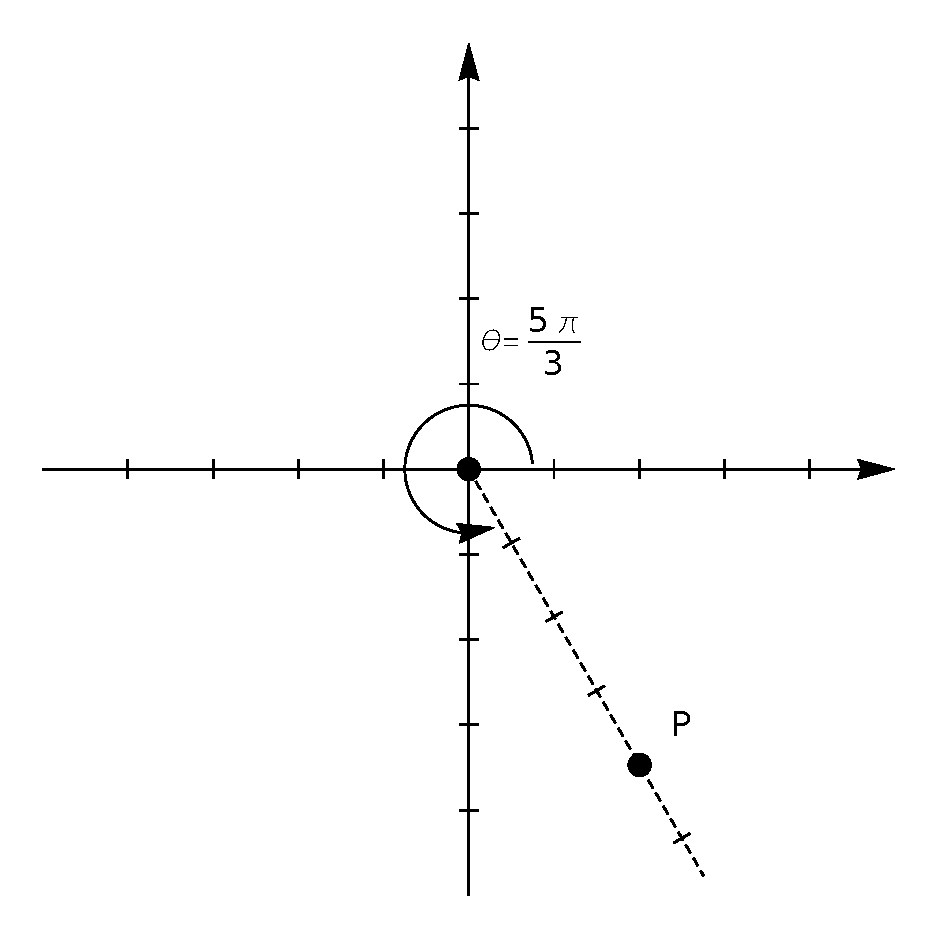
\includegraphics[width=0.33\textwidth]{fig_parametric_2a}}
\hspace{1cm}
\subfigure[\label{fig_parametric_2b}]{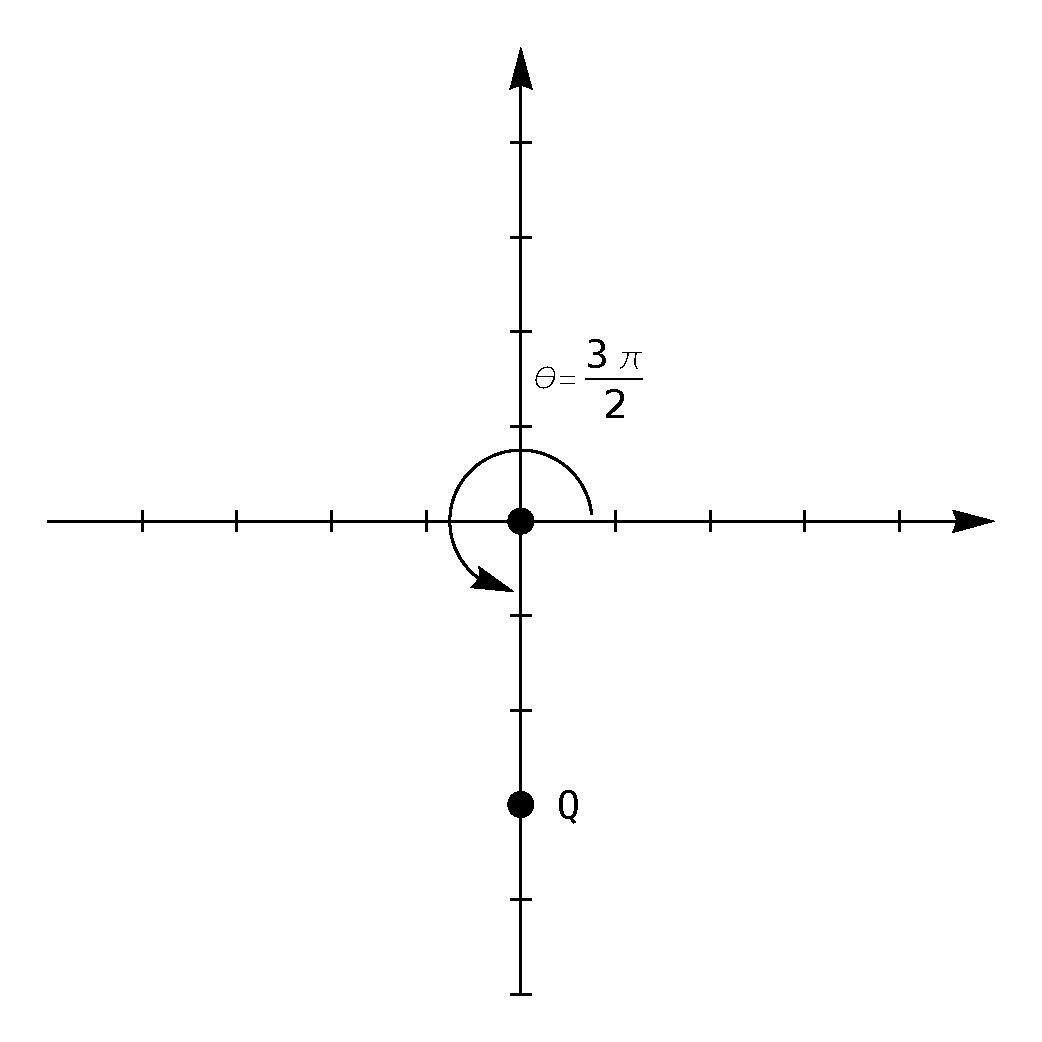
\includegraphics[width=0.33\textwidth]{fig_parametric_2b}}
}
\caption{The location of the point $P$ with rectangular coordinates $\left(2,-2\sqrt{3}\right)$ and polar coordinates $\left(4,\frac{5\pi}{3}\right)$ (a) and the point $Q$ with rectangular coordinates $\left(0,-3\right)$ and polar coordinates $\left(3\sqrt{2},\frac{5\pi}{4}\right)$ (b). }

\end{figure}


From the previous example, it is clear that it is important to know in which quadrant the point under investigation lies in order to infer the corresponding $\theta$. Instead of using the $\arctan$-function for that purpose and then figure out the correct angle, it is often more useful to use the $\atan2$-function (2-argument tangent). The $\atan2$ is defined as the angle in the Euclidean plane, given in radians, between the positive $x$-axis and the ray to the point $(x,y)\neq(0,0)$. The angles are signed, with counter-clockwise angles being positive, and clockwise ones being negative. In other words, $\atan2(y,x)$ is in the interval $[0,\pi]$ when $y>0$ and in $\left.\right]-\pi, 0\left[\right.$ when $y<0$.  \index{$\atan2$} \index[aut]{$\atan2$} The function is defined as:
\begin{equation}
\atan2(y,x)=\left\{
\begin{array}{lcl}
\arctan\left(\dfrac{y}{x}\right)&,&\text{ if }x>0\\[0.2cm]
\arctan\left(\dfrac{y}{x}\right)+\pi&,&\text{ if }x<0\wedge y\geq0\\[0.2cm]
\arctan\left(\dfrac{y}{x}\right)-\pi&,&\text{ if }x<0\wedge y<0\\[0.2cm]
\dfrac{\pi}{2}&,&\text{ if }x=0\wedge y>0\\[0.2cm]
-\dfrac{\pi}{2}&,&\text{ if }x=0\wedge y<0\\[0.2cm]
\text{undefined}&,&\text{ if }x=0\wedge y=0\\[0.2cm]
\end{array}
\right.
\end{equation}


Of course, we do not have to restrict to points when converting from the rectangular to the polar coordinate system. We can do the same with equations  using Theorem~\ref{polarrectangularconversion}.  In polar coordinates, we will end up with equations in the variables $r$ and $\theta$. The obvious strategy to convert an equation from rectangular to polar coordinates is to replace every occurrence of $x$ with $r\cos(\theta)$ and every occurrence of $y$ with $r\sin(\theta)$ and use identities to simplify. On the other hand,  converting equations from polar to rectangular coordinates is not as straightforward.  We could solve $r^2 = x^2 + y^2$ for $r$ to get $r = \pm \sqrt{x^2+y^2}$ and solving $\tan(\theta) = \frac{y}{x}$ requires the arctangent function to get  $\theta = \arctan\left(\frac{y}{x}\right) + \pi k$ for integers $k$.  Still, since neither of these expressions for $r$ and $\theta$ are especially user-friendly, we might resort to a second strategy involving the rearrangement of the given polar equation so that the expressions $r^2 = x^2+y^2$, $r\cos(\theta)=x$,  $r\sin(\theta)=y$ and/or $\tan(\theta) = \frac{y}{x}$ present themselves.


\begin{example}
\label{eqnconversionex}
\begin{enumerate}

\item \label{recteqntopolar} Convert each equation in rectangular coordinates into an equation in polar coordinates.

\begin{enumerate}

\item  \label{ris6costheta} $(x-3)^2 + y^2 = 9$

\item  \label{yisnegx} $y = -x$

\end{enumerate}

\item \label{polareqntorect} Convert each equation in polar coordinates into an equation in rectangular coordinates.


\begin{enumerate}

\item  \label{risneg3} $r = -3$

\item \label{cardioidtorect} $r = 1 - \cos(\theta)$

\end{enumerate}
\end{enumerate}

\xhrulefill{gray}{2.5pt}Solution \xhrulefill{gray}{2.5pt}

\begin{enumerate}

\item 

\begin{enumerate}

\item We start by substituting  $x = r\cos(\theta)$ and $y = r\sin(\theta)$ into $(x-3)^2 + y^2 = 9$ and then simplify.  With no real direction in which to proceed, we follow our mathematical instincts and see where they take us.
\[ \begin{array}{rrclr}

&(r\cos(\theta) - 3)^2+ (r\sin(\theta))^2 & = & 9& \\[3pt]
\Leftrightarrow&r^2\cos^2(\theta) - 6 r\cos(\theta) + 9 + r^2 \sin^{2}(\theta) & = &  9 \\[3pt]
\Leftrightarrow&r^2\left(\cos^2(\theta) + \sin^{2}(\theta)\right) - 6 r\cos(\theta) & = & 0 & \quad\text{(Subtract $9$ from both sides.)}\\[3pt]
\Leftrightarrow&r^2 - 6 r\cos(\theta) & = & 0 & \quad\text{(Since $\cos^2(\theta) + \sin^2(\theta) = 1$.)} \\[3pt]
\Leftrightarrow&r(r - 6 \cos(\theta)) & = & 0 &  \quad\text{(Factor.)} \\ \end{array} \]

We get $r = 0$ or $r = 6\cos(\theta)$.  From Section~\ref{sec_conic} we know that the equation $(x-3)^2 + y^2 = 9$ describes a circle, and since $r=0$ describes just a point (namely the pole/origin), we choose $r = 6\cos(\theta)$ for our final answer.

\item  Substituting $x = r\cos(\theta)$ and $y = r\sin(\theta)$ into $y=-x$ gives $r\sin(\theta)= -r\cos(\theta)$. Rearranging, we get  $r\cos(\theta) + r\sin(\theta) = 0$ or $r(\cos(\theta) + \sin(\theta)) = 0$.  This gives $r=0$ or $\cos(\theta) + \sin(\theta) = 0$.  Solving the latter equation for $\theta$, we get $\theta = -\frac{\pi}{4} + \pi k$ for integers $k$. We know $y=-x$ describes a line through the origin.  As before, $r=0$ describes the origin, but nothing else.  Consider the equation $\theta = -\frac{\pi}{4}$.  In this equation, the variable $r$ is free, meaning it can assume any and all values including $r=0$. If we imagine plotting points $(r, -\frac{\pi}{4})$  for all conceivable values of $r$ (positive, negative and zero), we are essentially drawing the line containing the terminal side of $\theta = -\frac{\pi}{4}$ which is none other than $y = -x$.  Hence, we can take as our final answer   $\theta = -\frac{\pi}{4}$ here.

\end{enumerate}

\item 

\begin{enumerate}

\item Starting with $r = -3$, we can square both sides to get  $r^2 = (-3)^2$ or $r^2 = 9$.  We may now substitute $r^2 = x^2+y^2$ to get the equation $x^2+y^2 = 9$.  As we have seen, squaring an equation does not, in general, produce an equivalent equation.  The concern here is that the equation $r^2 = 9$ might be satisfied by more points than $r = -3$.  On the surface, this appears to be the case since $r^2 = 9$ is equivalent to $r = \pm 3$, and not just $r=-3$.  However, any point with polar coordinates $(3,\theta)$ can be represented as $(-3,\theta + \pi)$, which means any point $(r,\theta)$ whose polar coordinates satisfy the relation $r = \pm 3$ has an equivalent representation -- meaning that they represent the same point in the plane -- which satisfies $r=-3$.


\item  Once again, we need to manipulate   $r = 1 - \cos(\theta)$ a bit before using the conversion formulas given in Theorem~\ref{polarrectangularconversion}.  We could square both sides of this equation to obtain an $r^2$ on the left hand side, but that does not result in something helpful for the right hand side.  Instead, we multiply both sides by $r$ to obtain  $r^{2} = r - r\cos(\theta)$.  We now have an $r^2$ and an $r\cos(\theta)$ in the equation, which we can easily handle, but we also have another $r$ to deal with.  Rewriting the equation as $r = r^{2} + r\cos(\theta)$ and squaring both sides yields $r^2 = \left(r^2 + r\cos(\theta)\right)^2$.  Substituting $r^2 = x^2 + y^2$ and $r\cos(\theta) = x$ gives   $x^2 + y^2 = \left(x^2 + y^2 + x\right)^2$.  Once again, we have performed some algebraic manoeuvres which may have altered the set of points described by the original equation.  First, we multiplied both sides by $r$.  This means that now $r=0$ is a viable solution to the equation.  In the original equation, $r = 1 - \cos(\theta)$, we see that $\theta = 0$ gives $r=0$, so the multiplication by $r$ does not introduce any new points.\\ The squaring of both sides of this equation is also a reason to pause.  Are there points with coordinates $(r,\theta)$ which satisfy $r^2 = \left(r^2 + r\cos(\theta)\right)^2$ but do not satisfy $r = r^2 + r\cos(\theta)$?  Suppose $\left(r',\theta'\right)$ satisfies $r^2 = \left(r^2 + r\cos(\theta)\right)^2$.  Then $r' = \pm \left((r')^2 + r'\cos(\theta')\right)$.  If we have that $r' = (r')^2 + r'\cos(\theta')$, we are done.  What if $r' = -\left((r')^2 + r'\cos(\theta')\right) = -(r')^{2} - r'\cos(\theta')$?  We claim that the coordinates $(-r', \theta' + \pi)$, which determine the same point as $(r',\theta')$, satisfy $r = r^2 + r\cos(\theta)$. We substitute $r =  -r'$ and $\theta = \theta' + \pi$ into $r = r^2 + r\cos(\theta)$ to see if we get a true statement.

\[ \begin{array}{rrclr}

&-r' & \stackrel{\text{?}}{=}  & \left(-r'\right)^2 + \left(-r' \cos(\theta' + \pi)\right) & \\ [5pt]

\Leftrightarrow&-\left(-(r')^2 - r'\cos(\theta') \right)   & \stackrel{\text{?}}{=}  & (r')^2 - r' \cos(\theta' + \pi) & \quad\text{(Since $r' = -(r')^{2} - r'\cos(\theta')$.)} \\[5pt]

\Leftrightarrow&(r')^2 + r'\cos(\theta') & \stackrel{\text{?}}{=}  & (r')^2 - r' (- \cos(\theta')) & \quad\text{(Since $\cos(\theta' + \pi) = -\cos(\theta')$.)} \\[5pt]

\Leftrightarrow&(r')^2 + r'\cos(\theta') & \stackrel{\text{\checkmark}}{=}  & (r')^2 + r' \cos(\theta') & \\

\end{array} \]

Since both sides worked out to be equal, $(-r', \theta' + \pi)$ satisfies $r = r^2 + r\cos(\theta)$, which means that any point $(r,\theta)$ that satisfies $r^2 = \left(r^2 + r\cos(\theta)\right)^2$ has a representation which satisfies  $r = r^2 + r\cos(\theta)$, and we are done.


\end{enumerate}

\end{enumerate}
\end{example}

In practice, much of the pedantic verification of the equivalence of equations in Example \ref{eqnconversionex} is left unsaid.  Indeed, in most textbooks, squaring equations like $r=-3$ to arrive at $r^2=9$ happens without a second thought. If you take anything away from Example \ref{eqnconversionex}, it should be that relatively nice things in rectangular coordinates, such as $y = x^2$, can turn ugly in polar coordinates, and vice-versa.


\subsection{Graphs of polar equations}

Having introduced polar coordinates and equations expressed therein, we now discuss how to graph equations in polar coordinates on the rectangular coordinate plane.  Since any given point in the plane has infinitely many different representations in polar coordinates, we have the following fundamental graphing principle.

\begin{definition}[The fundamental graphing principle for polar equations]
\label{fgpp}

The graph of an equation in polar coordinates is the set of points that satisfy the equation.  That is, a point $P(r,\theta)$ is on the graph of an equation if and only if there is a representation of $P$, say $\left(\widetilde{r},\widetilde{\theta}\right)$, such that $\widetilde{r}$ and $\widetilde{\theta}$ satisfy the equation.

\end{definition}

Our first example focuses on some of the more structurally simple polar equations.

\begin{example} \label{rthetaconstant} Graph the following polar equations.

\begin{multicols}{2}
\begin{enumerate}

\item  $r = 4$

\item  $\theta = -\dfrac{3\pi}{2}$

\end{enumerate}
\end{multicols}
\xhrulefill{gray}{2.5pt}Solution \xhrulefill{gray}{2.5pt}

\begin{enumerate}

\item  In the r equation, $\theta$ is free.  Its graph is, therefore,  all points which have a polar coordinate representation $(4,\theta)$, for any choice of $\theta$ (Figure~\ref{fig_parametric_3a}).  Graphically this translates into tracing out all of the points $4$ units away from the origin.  This is exactly the definition of circle, centred at the origin, with a radius of $4$ (Figure~\ref{fig_parametric_3b}).



\begin{figure}[H]
\centering
%\raisebox{0.5cm}{
\centerline{\subfigure[In $r=4$, $\theta$ is free.\label{fig_parametric_3a}]{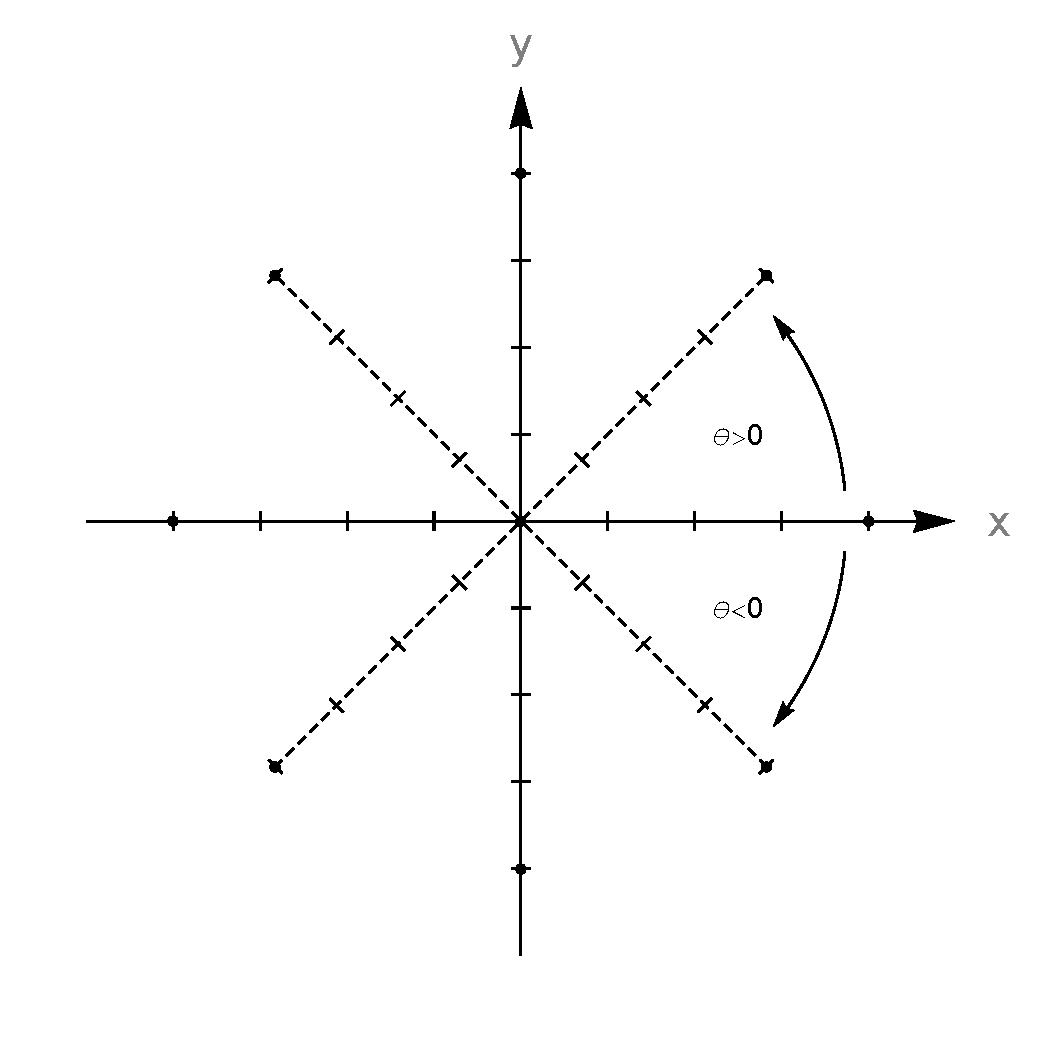
\includegraphics[width=0.43\textwidth]{fig_parametric_3a}}
\hspace{0.1cm}
\subfigure[The graph of $r=4$. \label{fig_parametric_3b}]{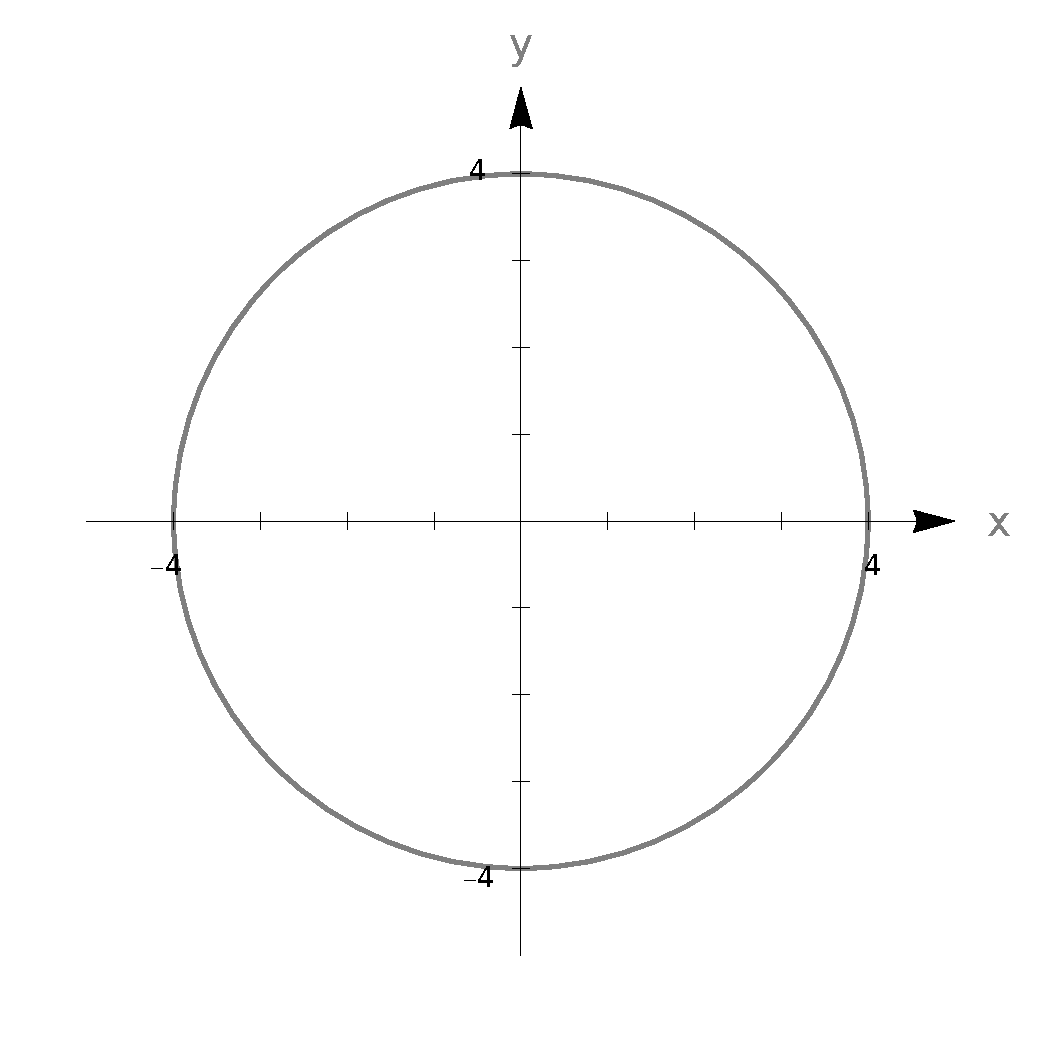
\includegraphics[width=0.43\textwidth]{fig_parametric_3b}}}
\caption{Constructing the graph of $r=4$.}
\end{figure}


\item  Here, the variable $r$ is free (Figure~\ref{fig_parametric_4a}).  Plotting $\left(r, -\frac{3\pi}{2}\right)$ for various values of $r$ shows us that we are tracing out the $y$-axis (Figure~\ref{fig_parametric_4b}).

\begin{figure}[H]
\centering
%\raisebox{0.5cm}{
\centerline{
\subfigure[In $\theta  = -\frac{3\pi}{2}$, $r$ is free.\label{fig_parametric_4a}]{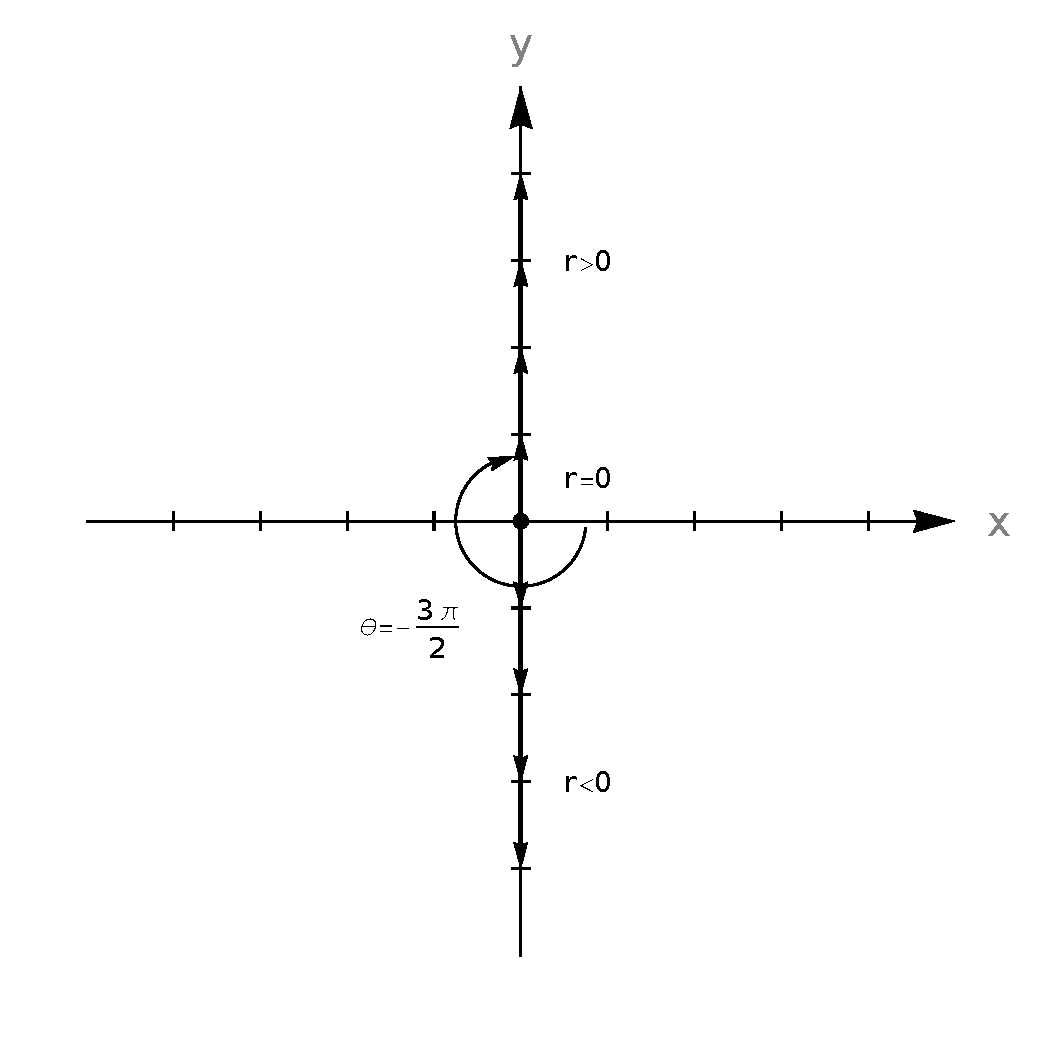
\includegraphics[width=0.43\textwidth]{fig_parametric_4a}}
\hspace{0.1cm}
\subfigure[The graph of $\theta  = -\frac{3\pi}{2}$. \label{fig_parametric_4b}]{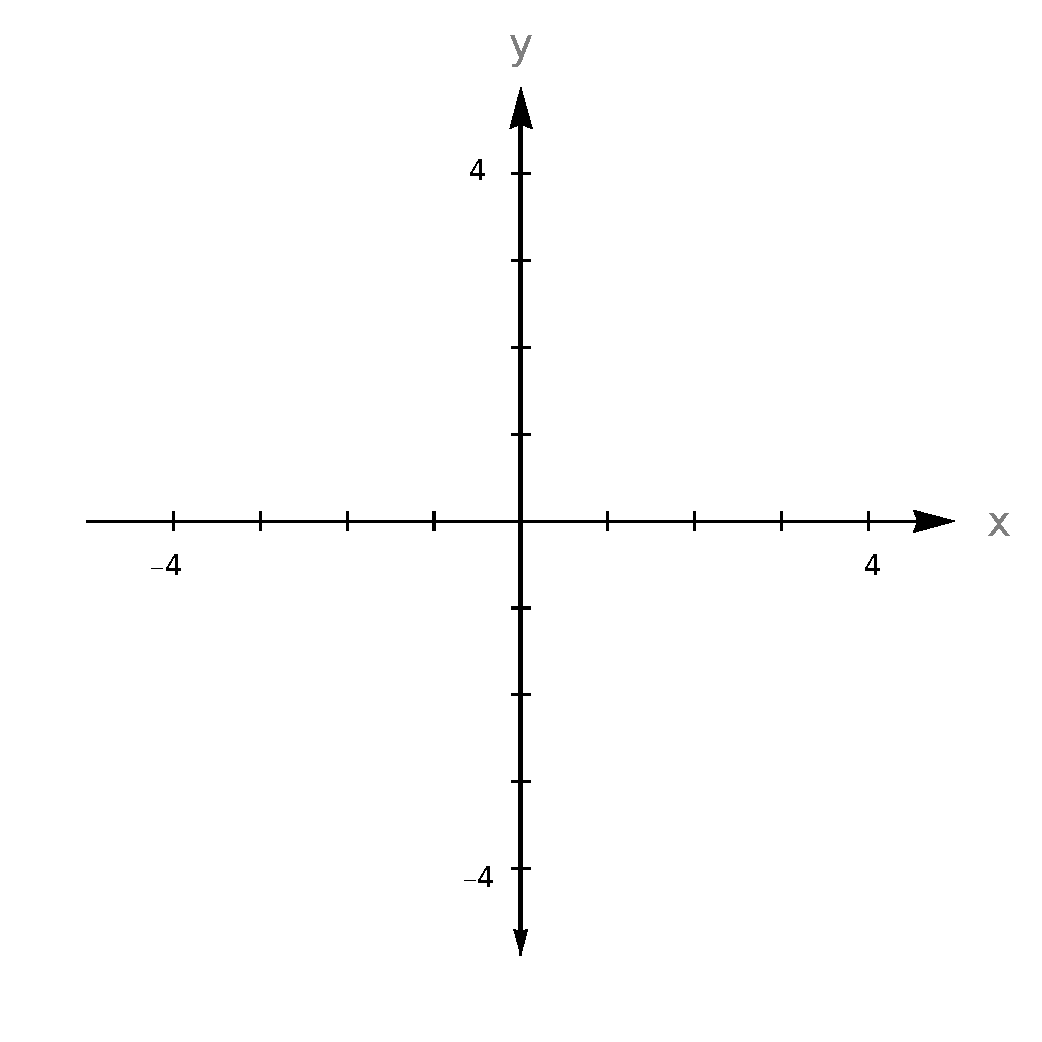
\includegraphics[width=0.43\textwidth]{fig_parametric_4b}}
}
\caption{Constructing the graph of $\theta  = -\frac{3\pi}{2}$. }

\end{figure}

\end{enumerate}
\end{example}

Our experience in Example~\ref{rthetaconstant} makes the following clear.
\begin{itemize}

\item The graph of the polar equation $r = a$ on the Cartesian plane is a circle centred at the origin of radius $|a|$.

\item The graph of the polar equation $\theta = \alpha$ on the Cartesian plane is the line containing the terminal side of $\alpha$ when plotted in standard position.


\end{itemize}
\ifmathematica
Since it gets way more involved to construct the graphs of generic polar equations, we will resort to Mathematica for that purpose. This programme also allows us to check analytically, for instance,  intersection of the graphs of multiple polar equations. More specifically, we can rely on the built-in function \lstinline{PolarPlot} to construct the graph of polar equations.
\fi
\ifpython
Since it gets way more involved to construct the graphs of generic polar equations, we will resort to Python for that purpose. This programme also allows us to check analytically, for instance,  intersection of the graphs of multiple polar equations.
\fi

\begin{example} \label{polargraphex}  Graph the following polar equations.

\begin{multicols}{2}
\begin{enumerate}

\item  \label{limacon01} $r = 4 - 2\sin(\theta)$ 

\item  \label{lemniscate} $r^2 = 16 \cos(2\theta)$

\end{enumerate}
\end{multicols}

\xhrulefill{gray}{2.5pt}Solution \xhrulefill{gray}{2.5pt}

\begin{enumerate}
\ifmathematica
\item We proceed in Mathematica using the following instruction, where we chose to indicate the axis labels and directions. 
\begin{mdframed}[default,backgroundcolor=gray!40,roundcorner=8pt]
\begin{mmaCell}[morefunctionlocal={theta},moredefined={PolarPlot,Arrowheads}]{Input}
  PolarPlot[4-2 Sin[theta],\{theta,0,2*Pi\}, AxesLabel->\{"x","y"\},
	 AxesStyle->Arrowheads[\{0,0.05\}]]
\end{mmaCell}



\begin{mmaCell}[moregraphics={moreig={scale=.4}}]{Output}
	 \mmaGraphics{fig_parametric_5}
\end{mmaCell}
\end{mdframed}
\fi

\ifpython
\item We proceed in Python using the following instruction, where we chose to indicate the axis labels.
\begin{pyin}
from sympy import symbols, diff, symbols, sin
from sympy.plotting import plot_parametric
theta = symbols('theta')
r = 4-2*sin(theta)
plot_parametric((r*cos(theta), r*sin(theta)), (theta, 0, 2*pi), xlabel="x", ylabel="y")
\end{pyin}
\begin{pyout}
|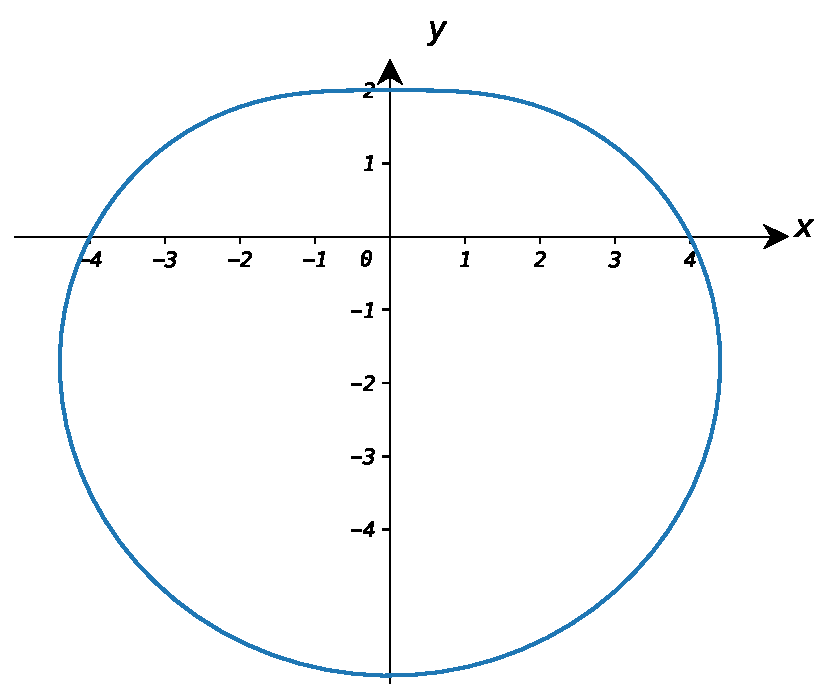
\includegraphics{figures/Parametric/fig_parametric_5_Python.pdf}|
\end{pyout}
\fi

Note that we chose $\theta$ to vary between 0 and $2\pi$ because the period of the concerned polar equation is $2\pi$. 
\item  Graphing $r^2 = 16 \cos(2\theta)$ is complicated by the $r^2$, so we solve to get $$r = \pm \sqrt{16 \cos(2\theta)} = \pm 4 \sqrt{\cos(2\theta)}.$$
Since the period of the involved cosine is $\pi$, we plot both functions together using \lstinline{PolarPlot} for $\theta\in[0,\pi]$.

\begin{mdframed}[default,backgroundcolor=gray!40,roundcorner=8pt]
\begin{mmaCell}[morefunctionlocal={theta},moredefined={PolarPlot,Arrowheads}]{Input}
  PolarPlot[\{Sqrt[16 Cos[2* theta]],- Sqrt[16 Cos[2*theta]]\},\{theta,0,Pi\},
	 AxesLabel->\{"x","y"\},AxesStyle->Arrowheads[\{0,0.05\}]]
\end{mmaCell}



\begin{mmaCell}[moregraphics={moreig={scale=.4}}]{Output}
	 \mmaGraphics{fig_parametric_6}
\end{mmaCell}
\end{mdframed}
Also note that we may plot values of  $\theta$ outside of the interval $[0,\pi]$, but then we will  find ourselves retracing parts of the curve we already had obtained. 
\end{enumerate}

\end{example}

The previous example makes us appreciate the symmetry that is a common occurrence when graphing polar equations.  Indeed, it can be verified easily that $r=f(\theta)$ is symmetric about the $x$-axis if $f$ is even because then we have that $f(\theta)=f(-\theta)$ (e.g. Example~\ref{polargraphex}.2), symmetric about the $y$-axis if $f(\pi-\theta)=f(\theta)$ (e.g. Example~\ref{polargraphex}.1 and 2) and symmetric about the origin if $f$ is odd because then we have that $f(-\theta)=-f(\theta)$ (e.g. Example~\ref{polargraphex}.2).  In addition these usual kinds of symmetry, it is possible to talk about rotational symmetry. More specifically, if $f(\theta - \alpha) = f(\theta)$ it will be rotationally symmetric by $\alpha$ clockwise and counter-clockwise about the pole. 


\index{function ! odd}\index{odd function} \index[aut]{functie ! oneven}\index[aut]{oneven functie}
\index{function ! even}\index{even function} \index[aut]{functie ! even}\index[aut]{even functie}

 In our next example, we are given the task of finding the intersection points of polar curves.


\begin{example}  \label{polargraphintex} Find the points of intersection of the graphs of the following polar equations.

\begin{multicols}{2}
\begin{enumerate}

\item  \label{circcardint} $r =2\sin(\theta)$ and $r = 2 - 2\sin(\theta)$

\item \label{circroseint} $r=3$ and  $r = 6\cos(2\theta)$

\end{enumerate}
\end{multicols}

\xhrulefill{gray}{2.5pt}Solution \xhrulefill{gray}{2.5pt}

\begin{enumerate}
\item  We first try to see if we can find any points which have a single representation $P(r,\theta)$ that satisfies both equations.  Assuming such a pair $(r,\theta)$ exists, then equating the expressions for $r$ gives \begin{eqnarray*}
2\sin(\theta) = 2-2\sin(\theta)&\Leftrightarrow&\sin(\theta) = \frac{1}{2}\\
&\Leftrightarrow&\theta = \frac{\pi}{6} + 2\pi k \text{ or }\theta = \frac{5\pi}{6} + 2\pi k
\end{eqnarray*}
for integers $k$.  Plugging $\theta = \frac{\pi}{6}$ into $r = 2\sin(\theta)$, we get $r = 2\sin\left(\frac{\pi}{6}\right) = 2\left(\frac{1}{2}\right) = 1$, which is also the value we obtain when we substitute it into $r = 2-2\sin(\theta)$.  Hence, $\left(1, \frac{\pi}{6}\right)$ is one representation for the point of intersection in quadrant I. For the point of intersection in Quadrant II, we try $\theta = \frac{5\pi}{6}$. Both equations give us the point $\left(1, \frac{5\pi}{6}\right)$, so this is our answer here. Now, let us check graphically whether we indeed found all intersection points of the graphs of the involved polar equations.  (Figure~\ref{fig_parametric_7a}). 

From this graph it appears that there are three intersection points:  one in Quadrant I, one in Quadrant II, and the origin. So, how to find the latter algebraically? We know that the pole may be represented as $(0,\theta)$ for any angle $\theta$. On the graph of $r = 2\sin(\theta)$, we start at the origin when $\theta =0$ and return to it at $\theta = \pi$. Actually, we are at the origin exactly when $\theta = \pi k$ for integers $k$. On the curve $r = 2 - 2\sin(\theta)$, however, we reach the origin when $\theta = \frac{\pi}{2}$, and more generally, when $\theta = \frac{\pi}{2} + 2\pi k$ for integers $k$.  There is no integer value of $k$ for which $\pi k = \frac{\pi}{2} + 2\pi k$, which means while the origin is on both graphs, the point is never reached simultaneously.  In any case, we have determined the three points of intersection to be $\left(1, \frac{\pi}{6}\right)$, $\left(1,\frac{5\pi}{6}\right)$ and the origin. 
\begin{figure}[H]
\centering
%\raisebox{0.5cm}{
\centerline{
\subfigure[$r =2\sin(\theta)$ (solid) and $r = 2 - 2\sin(\theta)$ (dashed).\label{fig_parametric_7a}]{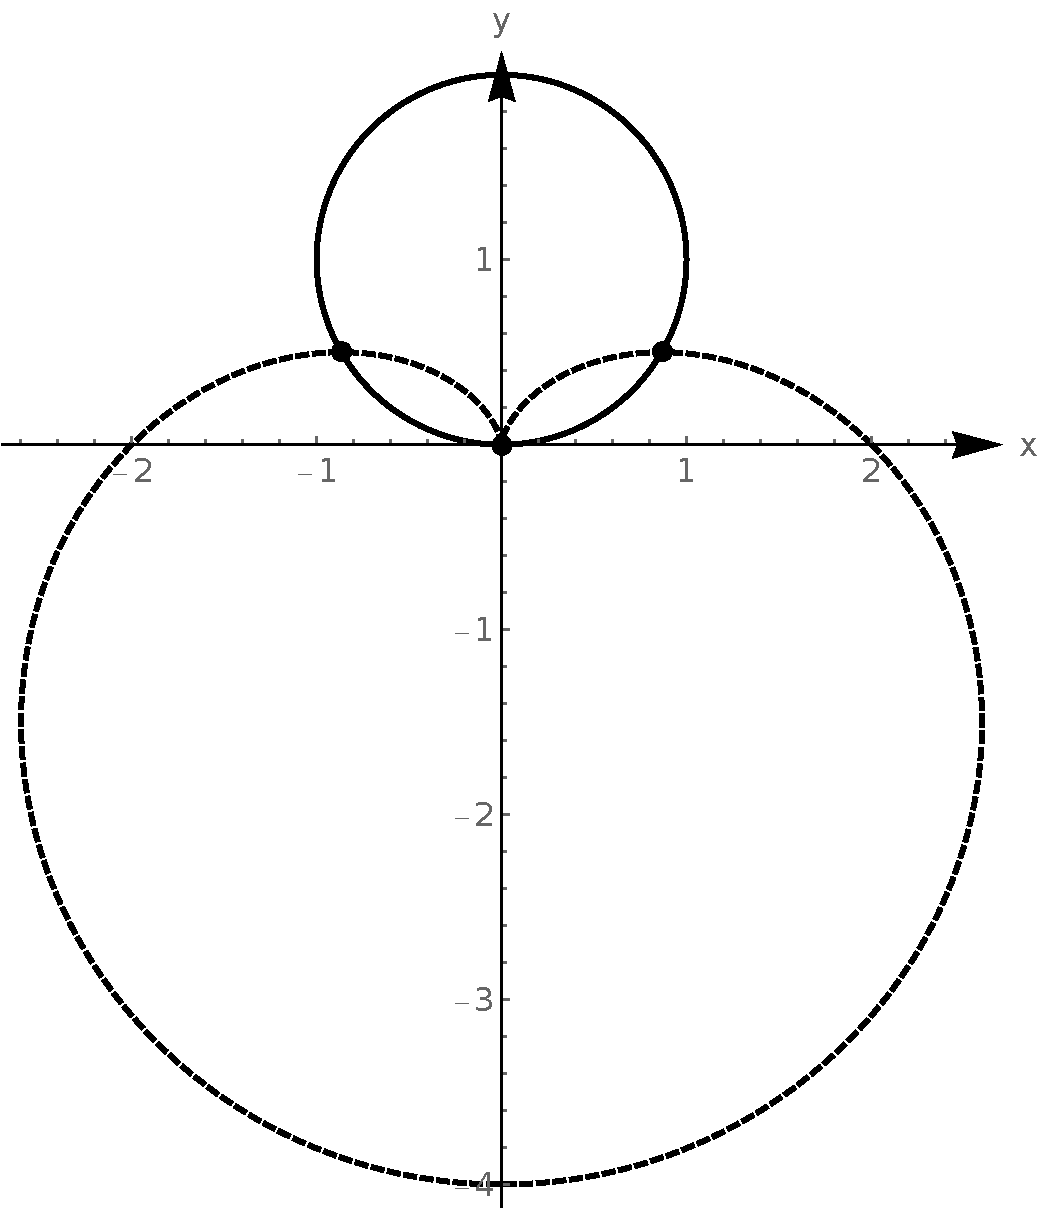
\includegraphics[width=0.3\textwidth]{fig_parametric_7a}}
\hspace{0.1cm}
\subfigure[$r=3$ (solid) and  $r = 6\cos(2\theta)$ (dashed). \label{fig_parametric_7b}]{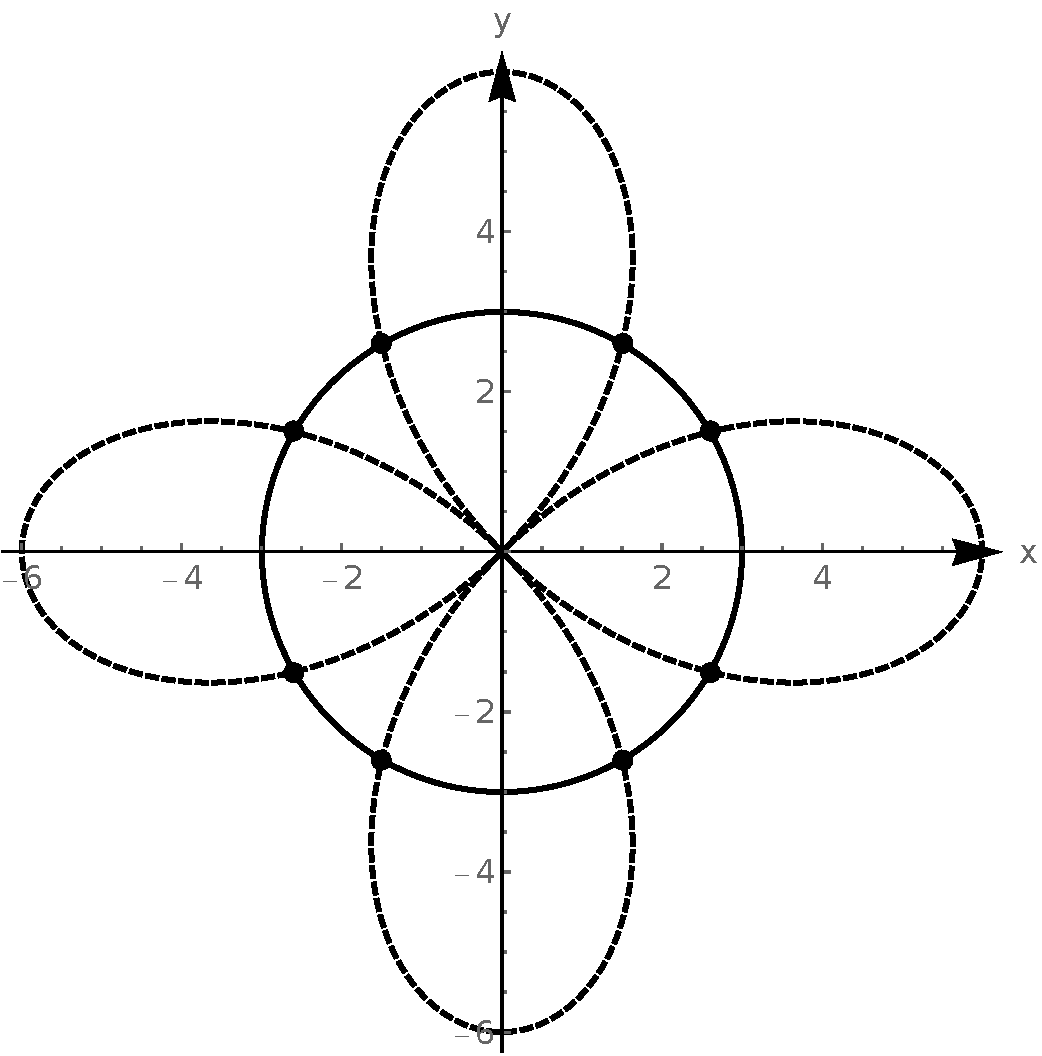
\includegraphics[width=0.33\textwidth]{fig_parametric_7b}}
}
\caption{Points of intersection of the graphs of two polar equations. }

\end{figure}


\item  Let us graph the equations  to get an idea of how many intersection points to expect and where they lie.  The graph of $r=3$ is a circle centred at the origin with a radius of $3$ and the graph of $r = 6\cos(2\theta)$ is 
a four-leafed rose (Figure~\ref{fig_parametric_7b}).

It appears as if there are eight points of intersection - two in each quadrant. We first look to see if there any points $P(r,\theta)$ with a representation that satisfies both equations.  For these points,  
\begin{eqnarray*}
6\cos(2\theta) = 3&\Leftrightarrow&\cos(2\theta) = \frac{1}{2}\\
&\Leftrightarrow&\theta = \frac{\pi}{6} + \pi k \text{ or } \theta = \frac{5\pi}{6} + \pi k
\end{eqnarray*}
for integers $k$.  Out of all of these solutions, we obtain just four distinct points represented by  $\left(3, \frac{\pi}{6}\right)$, $\left(3, \frac{5\pi}{6} \right)$, $\left(3, \frac{7\pi}{6}\right)$ and $\left(3, \frac{11\pi}{6} \right)$.  To determine the coordinates of the remaining four points, we have to consider how the representations of the points of intersection can differ.  We know from the beginning of this section that if $(r,\theta)$ and $(r', \theta')$ represent the same point and $r \neq 0$, then either $r = r'$ or $r = -r'$.  If $r = r'$, then $\theta' = \theta + 2\pi k$, so one possibility is that an intersection point $P$ has a representation $(r,\theta)$ which satisfies $r=3$  and another representation $(r, \theta + 2\pi k)$ for some integer $k$, which satisfies $r = 6\cos(2\theta)$.  At this point, if we replace every occurrence of $\theta$ in the equation $r=6\cos(2\theta)$ with $(\theta + 2\pi k)$ and then see if, by equating the resulting expressions for $r$, we get any more solutions for $\theta$. Since $\cos(2(\theta + 2\pi k)) = \cos(2\theta + 4\pi k) = \cos(2\theta)$ for every integer $k$, however, the equation $r = 6\cos(2(\theta + 2\pi k))$ reduces to the same equation we had before, $r = 6\cos(2\theta)$,  which means we get no additional solutions.\\     Moving on to the case where $r = -r'$, we have that $\theta' = \theta + (2k+1)\pi$ for integers $k$.  We look to see if we can find points $P$ which have a representation $(r,\theta)$ that satisfies $r=3$  and another, $(-r, \theta + (2k+1)\pi)$, that satisfies  $r = 6\cos(2\theta)$.  To do this, we substitute   $(-r)$ for $r$ and  $(\theta + (2k+1)\pi)$ for $\theta$ in the equation $r = 6\cos(2\theta)$ and get $-r = 6\cos(2(\theta + (2k+1)\pi))$.  Since $\cos(2(\theta + (2k+1)\pi)) = \cos(2\theta + (2k+1)(2\pi)) = \cos(2\theta)$ for all integers $k$, the equation $-r = 6\cos(2(\theta + (2k+1)\pi))$ reduces to $-r = 6\cos(2\theta)$, or $r = -6\cos(2\theta)$.   Coupling this equation with  $r=3$ gives
\begin{eqnarray*}
-6\cos(2\theta) = 3&\Leftrightarrow&\cos(2\theta) = -\frac{1}{2}\\
&\Leftrightarrow&\theta = \frac{\pi}{3} + \pi k\text{ or }\theta = \frac{2\pi}{3} + \pi k
\end{eqnarray*}
From these solutions, we obtain the remaining four intersection points with representations $\left(-3, \frac{\pi}{3}\right)$,  $\left(-3, \frac{2\pi}{3}\right)$,  $\left(-3, \frac{4\pi}{3}\right)$ and  $\left(-3, \frac{5\pi}{3}\right)$
\end{enumerate}





\end{example}

There are a number of basic and classic polar curves, famous for their beauty and/or applicability in science. For that reason, this section ends with a small gallery of some of these graphs.

\newlength{\gallerywidth}
\setlength{\gallerywidth}{(0pt+\marginparwidth+\textwidth)/4}
\rule{25pt+\marginparwidth+\textwidth}{1pt}\\


\textbf{\large Lines}\\


\begin{tabular}{cccc}
\textbf{Through the origin:} & \textbf{Horizontal line:} & \textbf{Vertical line:} & \textbf{Not through origin:} \\[5pt]
$\theta = \alpha$ & $r=a\csc(\theta)$ & $r=a\sec(\theta)$ & $\ds r=\frac{b}{\sin(\theta)-m\cos(\theta)}$ \\[10pt]
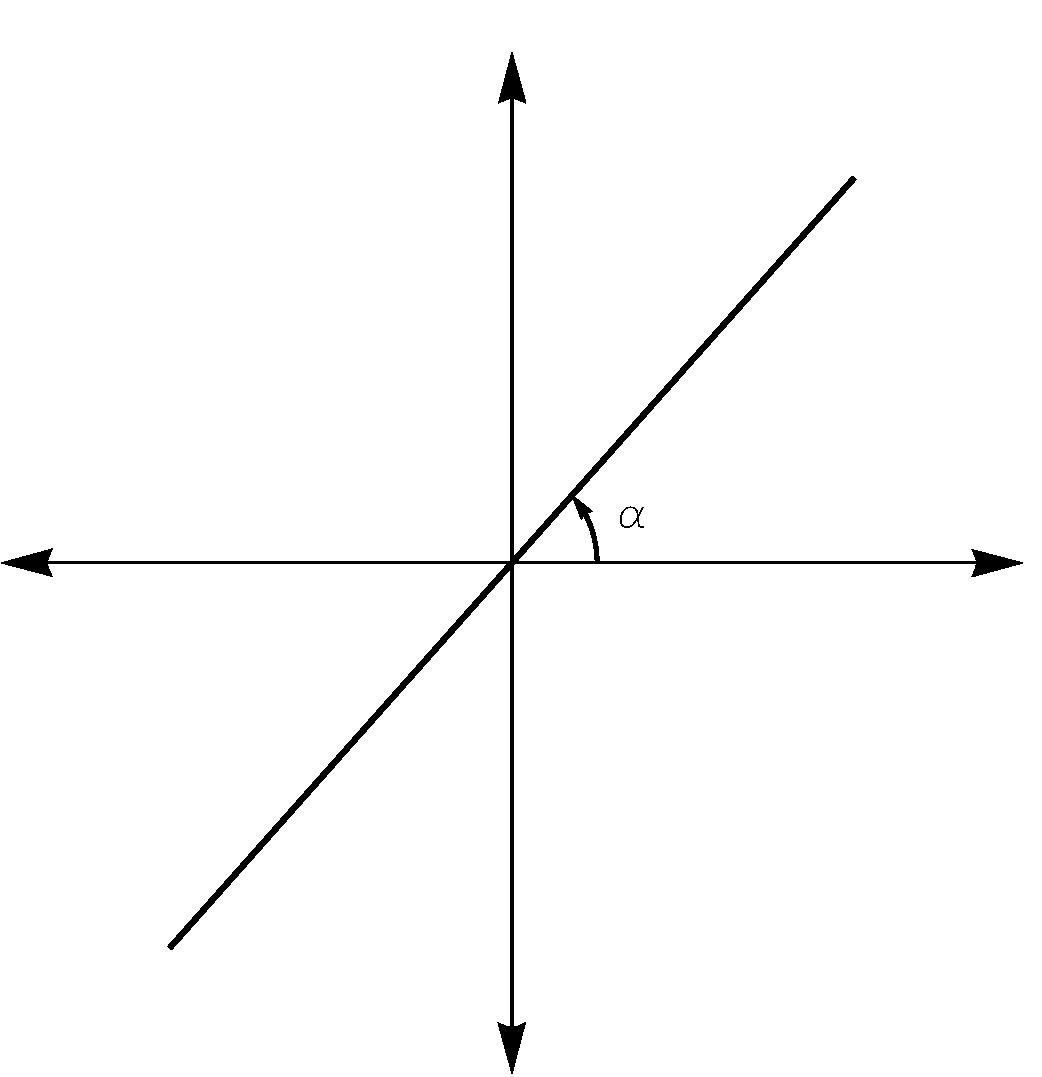
\includegraphics[width=.22\textwidth]{fig_parametric_8a} & 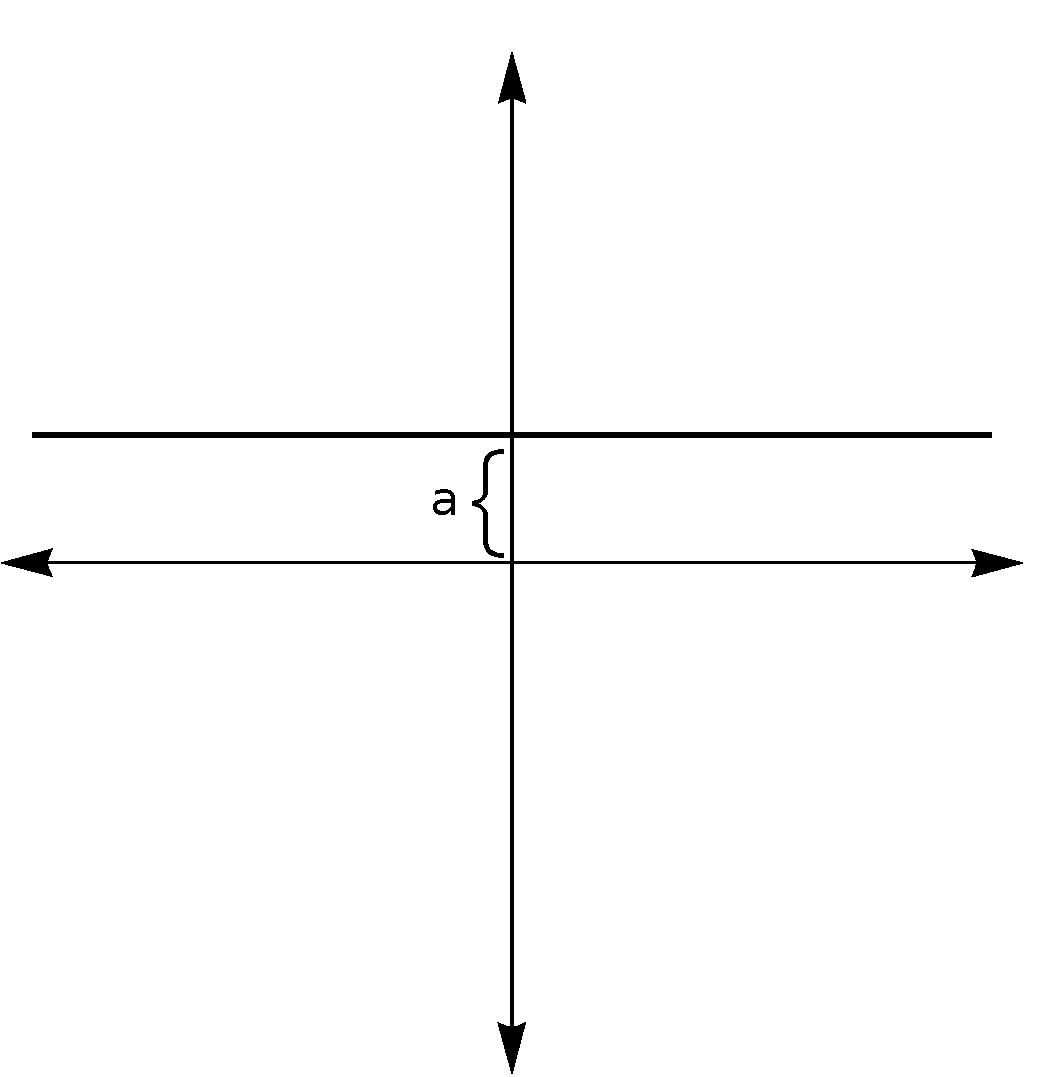
\includegraphics[width=.22\textwidth]{fig_parametric_8b} & 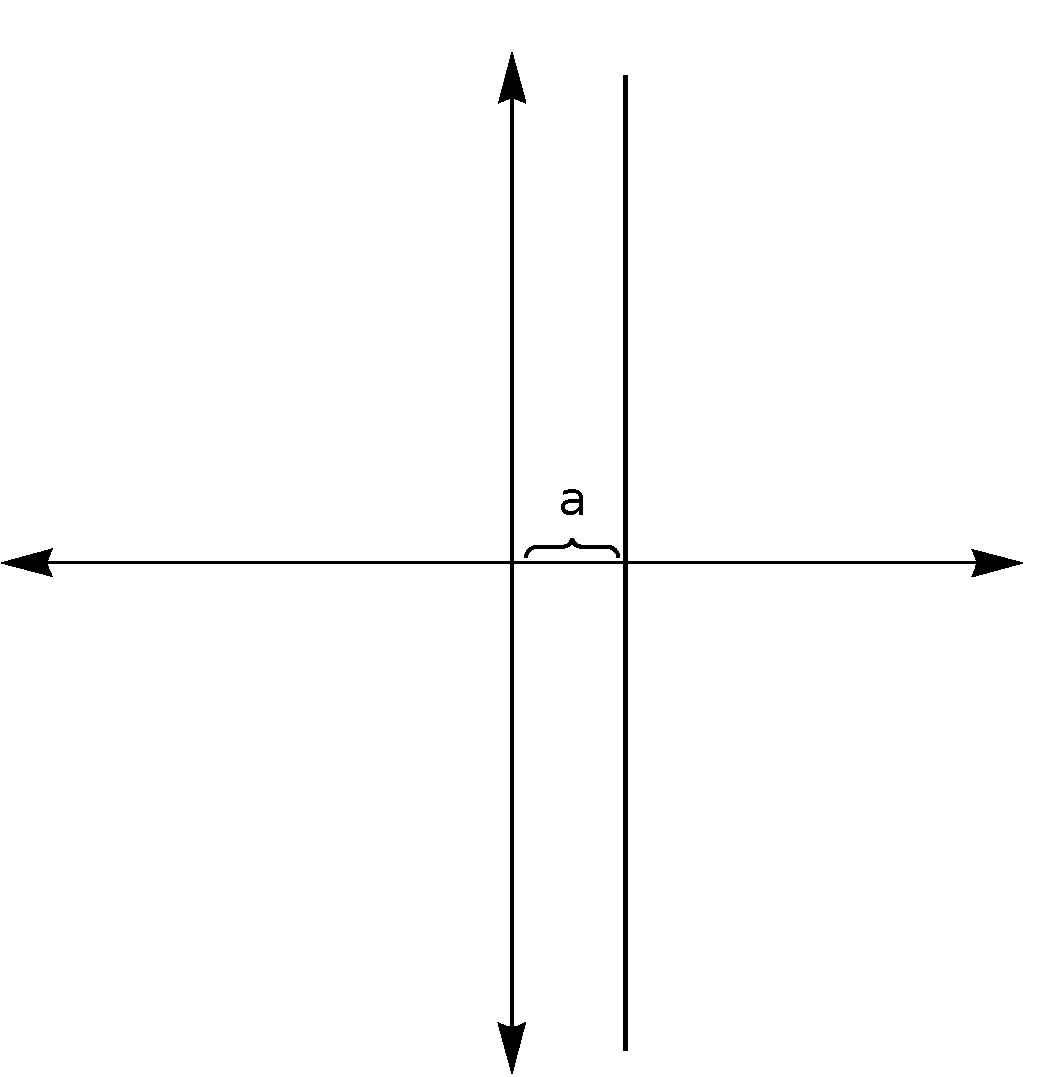
\includegraphics[width=.22\textwidth]{fig_parametric_8c} & 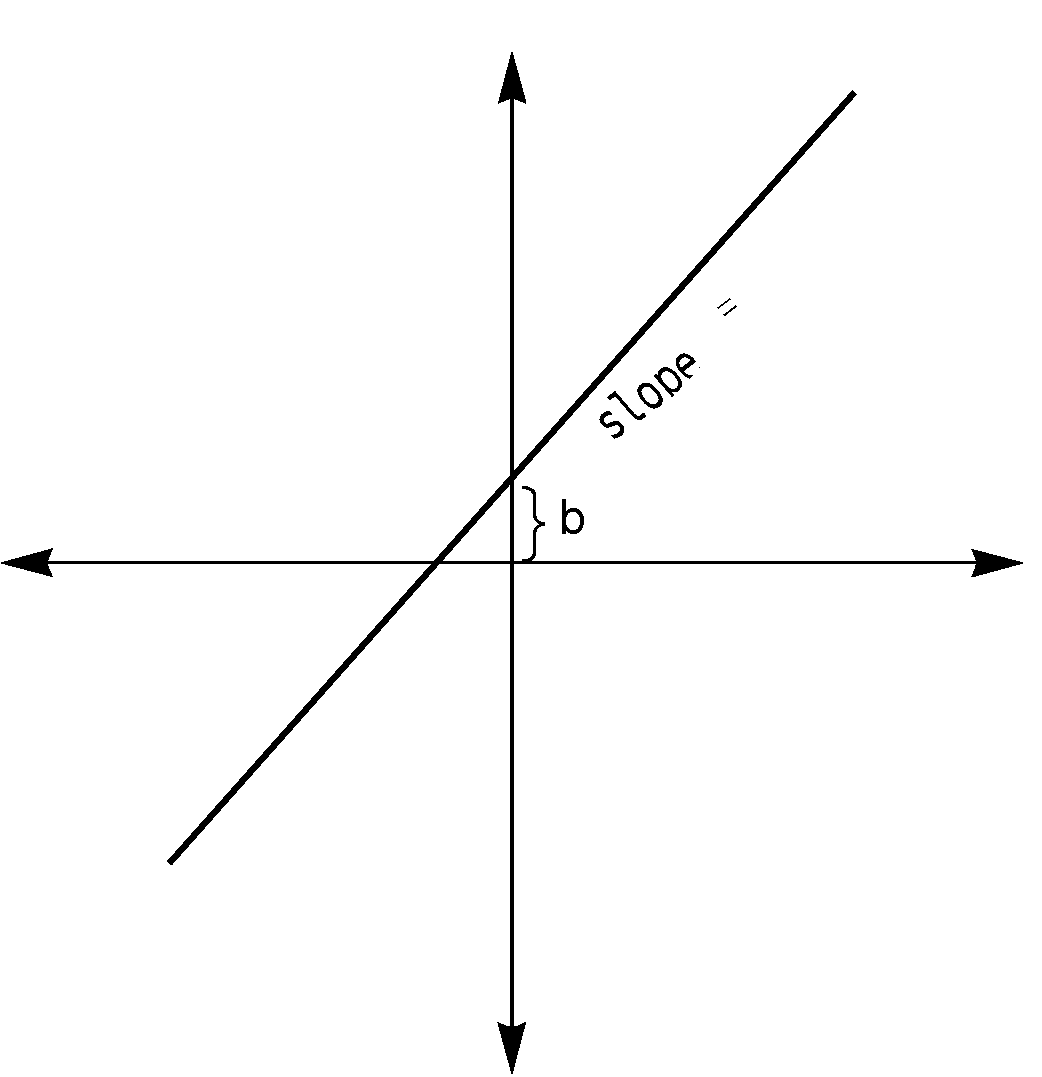
\includegraphics[width=.22\textwidth]{fig_parametric_8d}
\end{tabular}

\noindent\parbox{3\gallerywidth+37pt}{\textbf{\large Circles}}\textbf{\large Spiral}\\


\begin{tabular}{cccc}
\textbf{Centred on $x$-axis:} & \textbf{Centred on $y$-axis:} & \textbf{Centred on origin:} &\textbf{Archimedean spiral}\\
$r=a\cos (\theta)$ & $r=a\sin(\theta)$ & $r=a$ & $r=\theta$\\
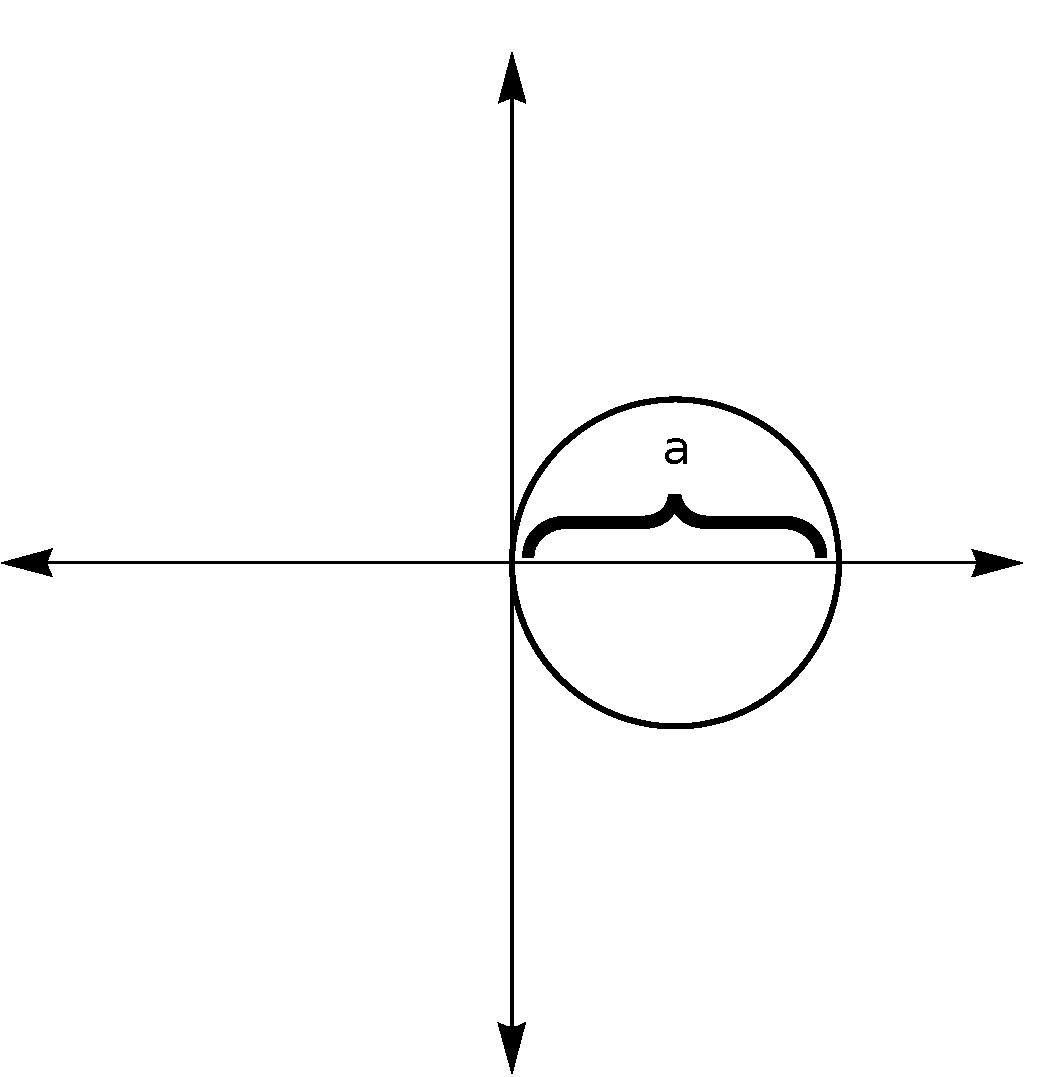
\includegraphics[width=.22\textwidth]{fig_parametric_9a}&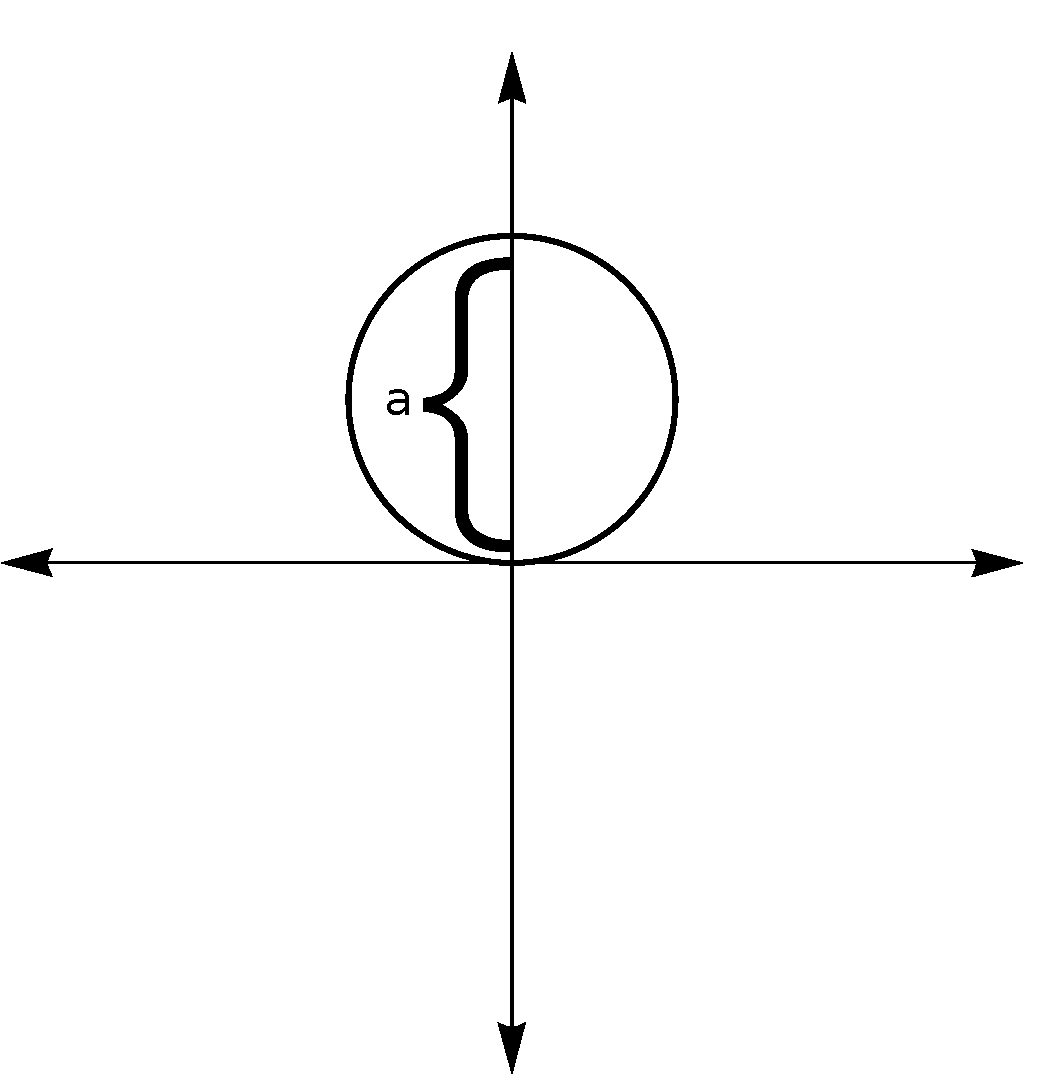
\includegraphics[width=.22\textwidth]{fig_parametric_9b}&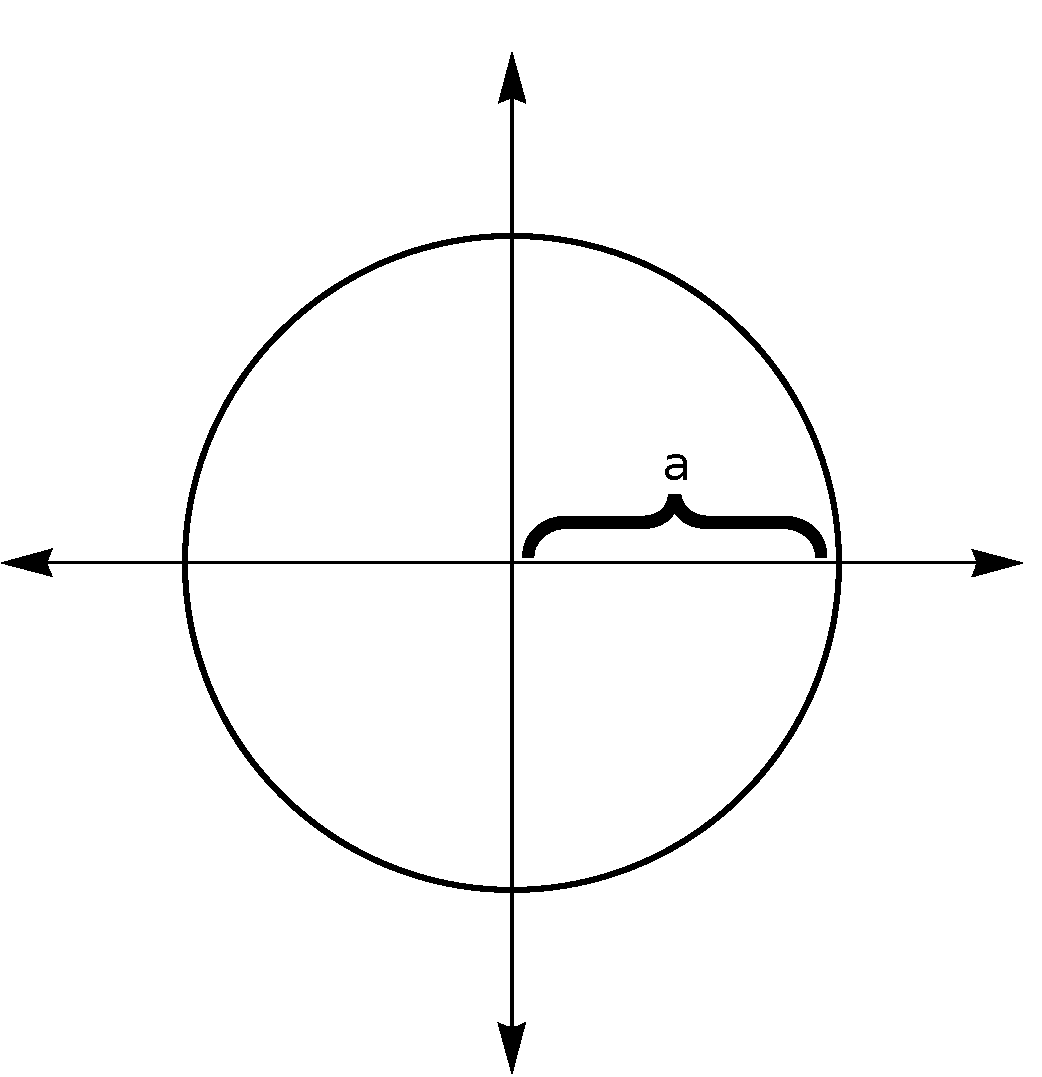
\includegraphics[width=.22\textwidth]{fig_parametric_9c}&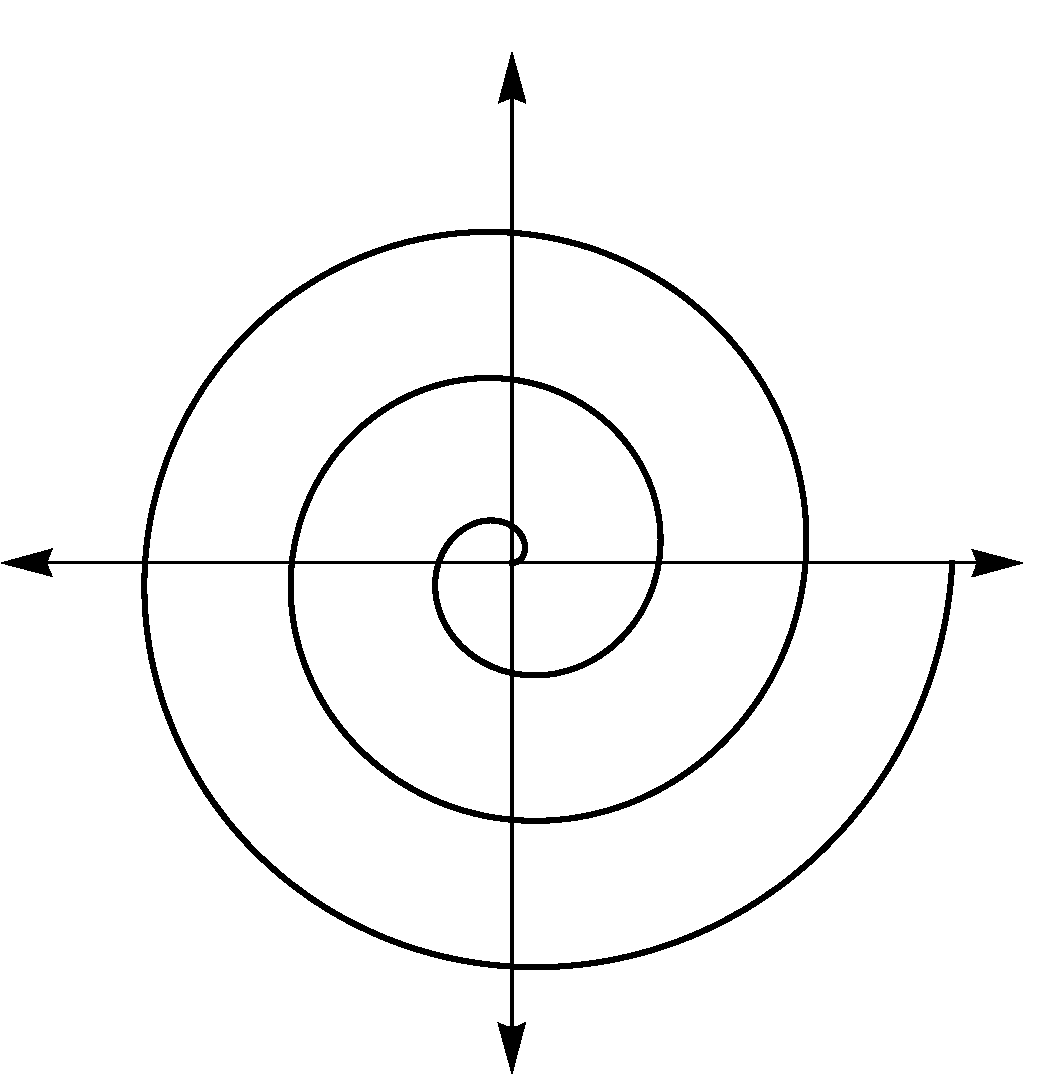
\includegraphics[width=.22\textwidth]{fig_parametric_9d}
\end{tabular}

\pagebreak
\noindent\textbf{\large Lima\c cons}\\

\parbox{4\gallerywidth}{Symmetric about $x$-axis: $r=a\pm b\cos(\theta)$; \quad Symmetric about $y$-axis:  $r=a\pm b\sin (\theta)$; \quad $a,b>0$}\\


\begin{tabular}{cccc}
\textbf{With inner loop:} & \textbf{Cardioid:} & \textbf{Dimpled:} & \textbf{Convex:} \\[5pt]
$\ds \frac ab < 1$ & $\ds \frac ab=1$ & $\ds 1<\frac ab <2$ & $\ds \frac ab>2$ \\[10pt]
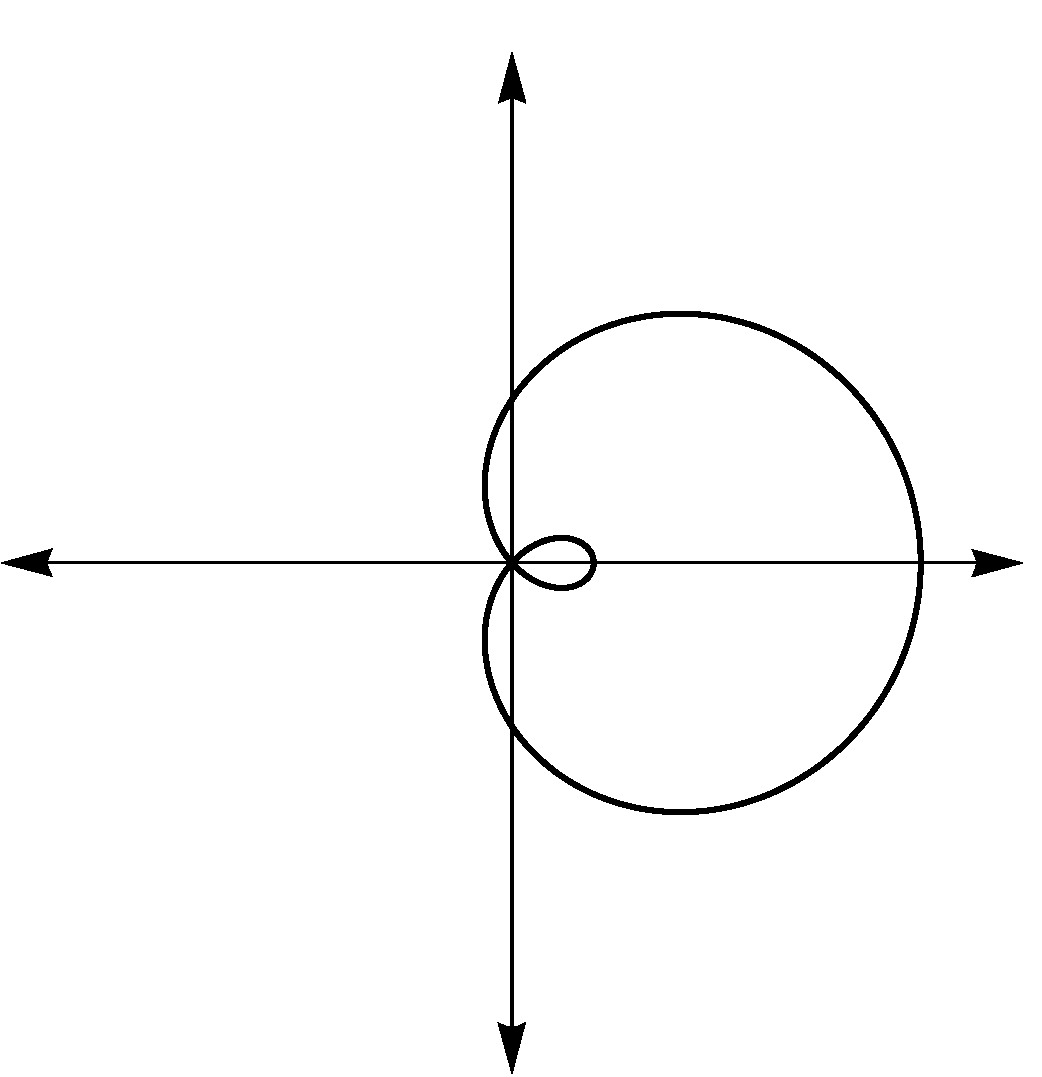
\includegraphics[width=.22\textwidth]{fig_parametric_10a} & 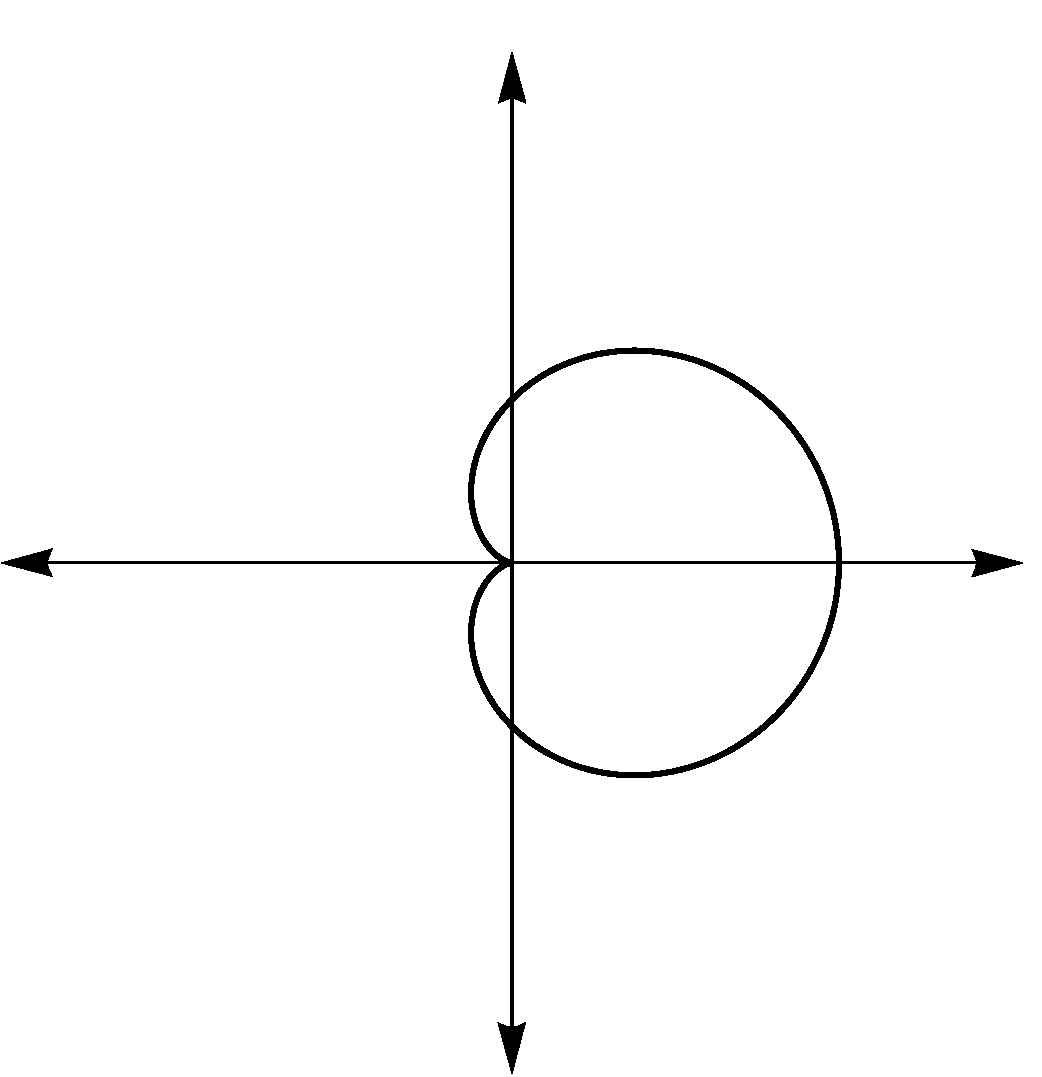
\includegraphics[width=.22\textwidth]{fig_parametric_10b} & 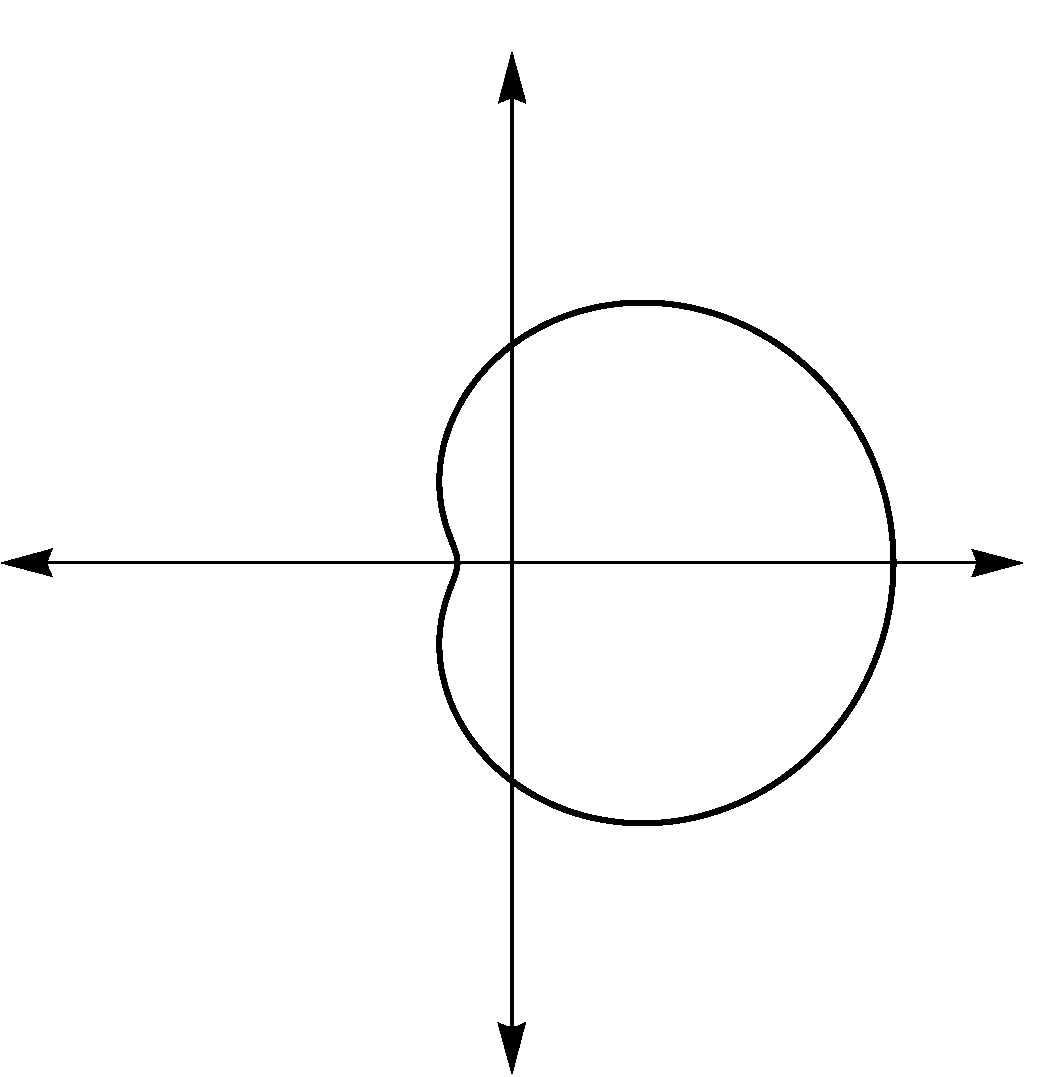
\includegraphics[width=.22\textwidth]{fig_parametric_10c} & 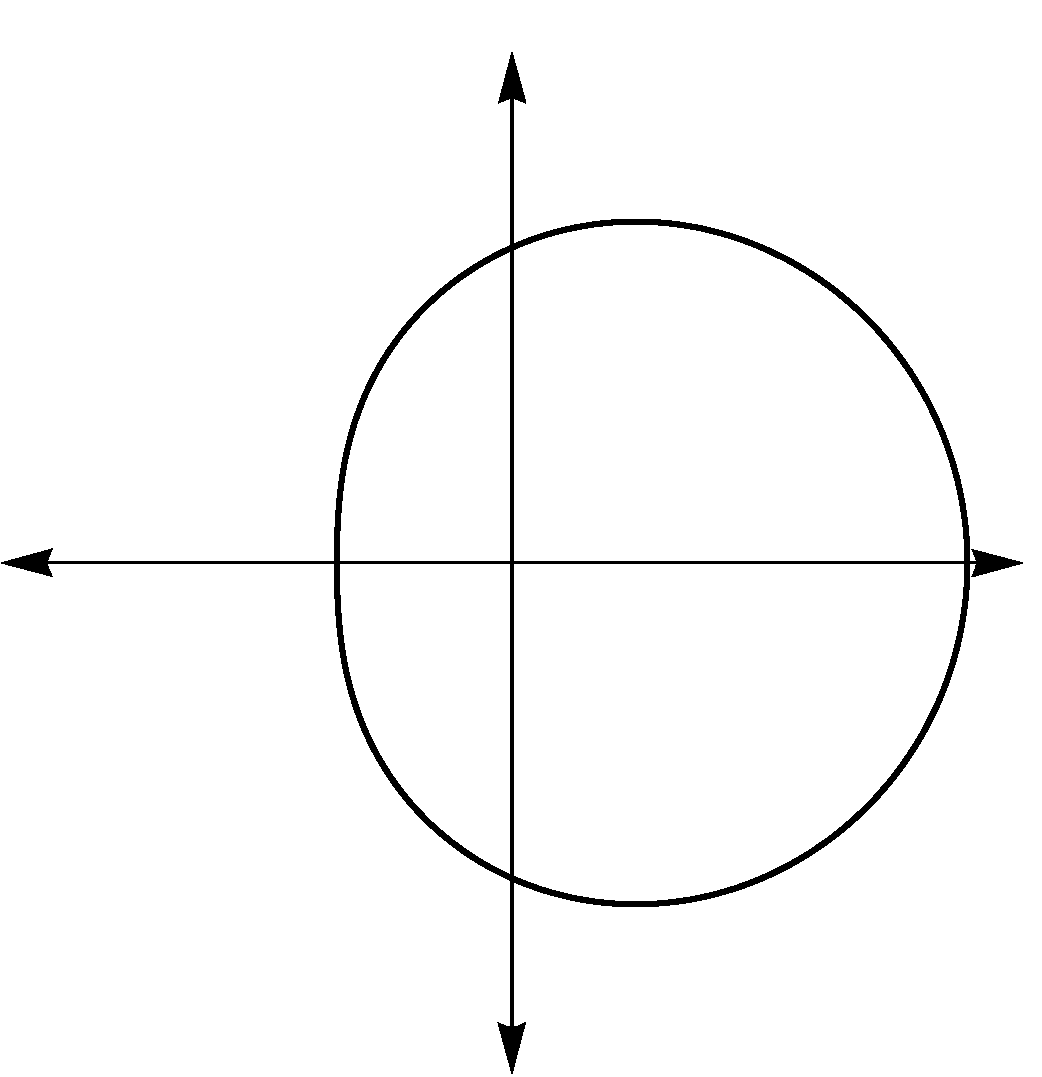
\includegraphics[width=.22\textwidth]{figures/Parametric/fig_parametric_10d.pdf}
\end{tabular}


\noindent\textbf{\large Rose Curves}\\
\label{Rose_curves}
\parbox{4\gallerywidth}{Symmetric about $x$-axis: $r=a \cos(n\theta)$; \quad Symmetric about $y$-axis:  $r=a\sin(n\theta)$}\\
\parbox{4\gallerywidth}{Curve contains $2n$ petals when $n$ is even and $n$ petals when $n$ is odd.}\\

\begin{tabular}{cccc}
%\textbf{With inner loop:} & \textbf{Cardioid:} & \textbf{Dimpled:} & \textbf{Convex:} \\[5pt]
$r=a\cos (2\theta)$ & $r=a\sin(2\theta)$ & $r=a\cos (3\theta)$ & $r=a\sin (3\theta)$ \\[10pt]
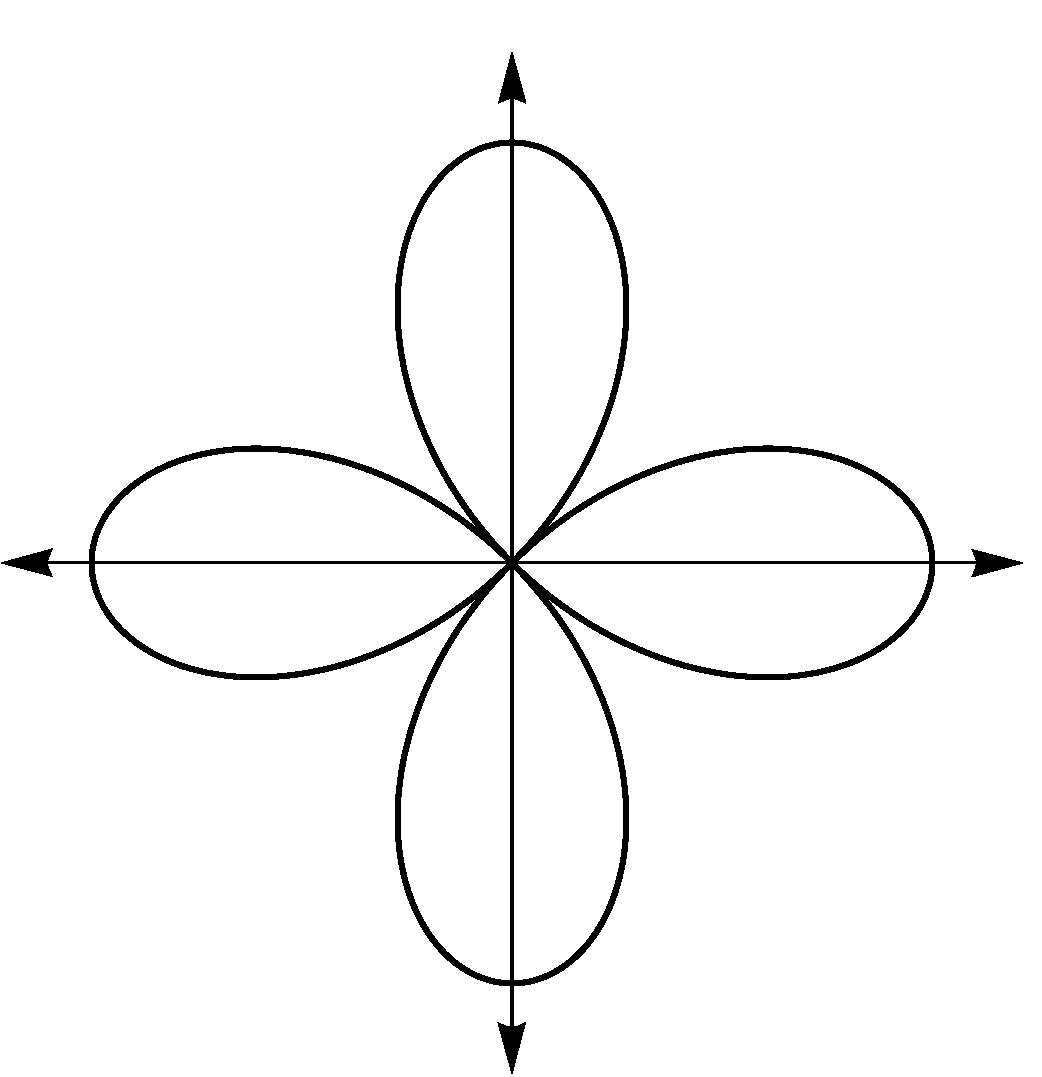
\includegraphics[width=.22\textwidth]{fig_parametric_11a} & 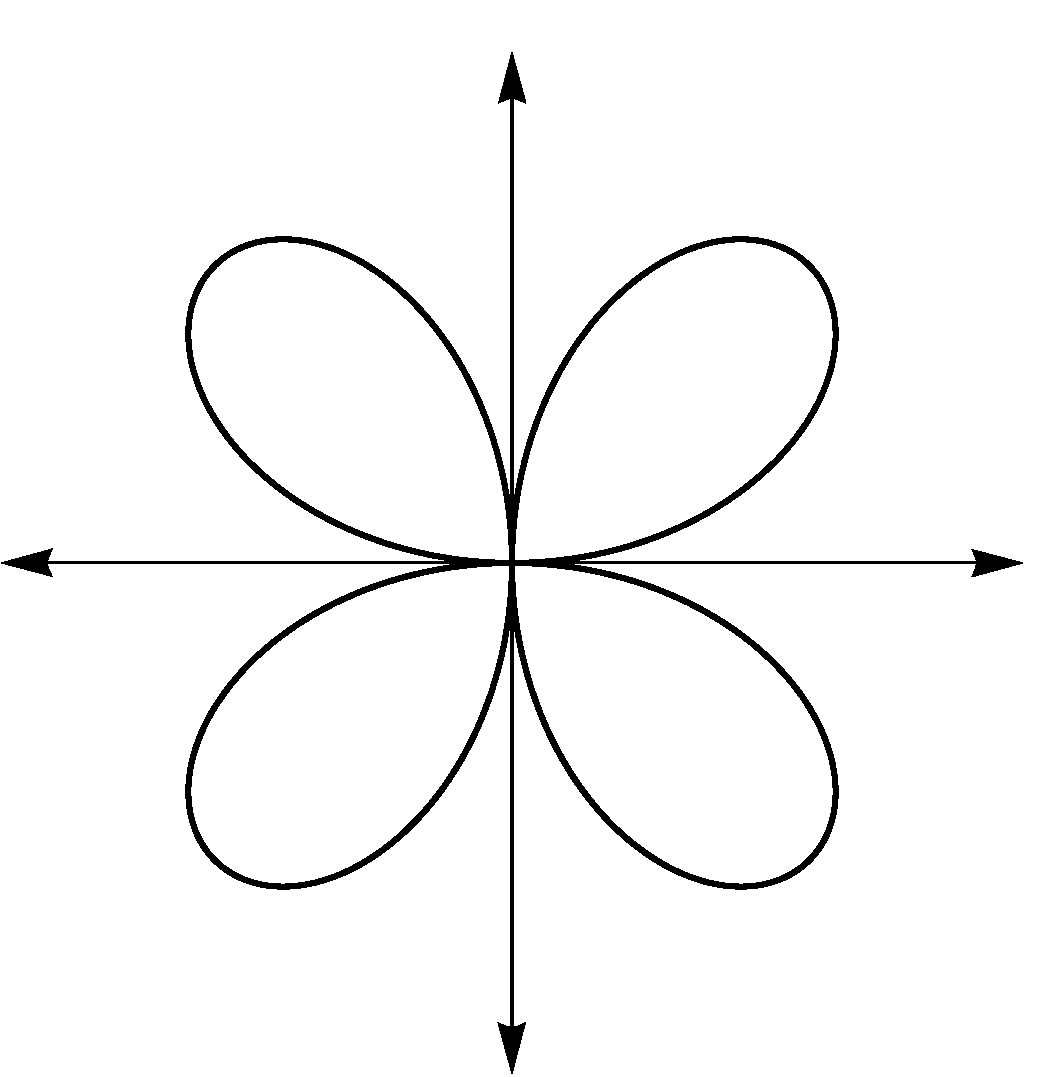
\includegraphics[width=.22\textwidth]{fig_parametric_11b} & 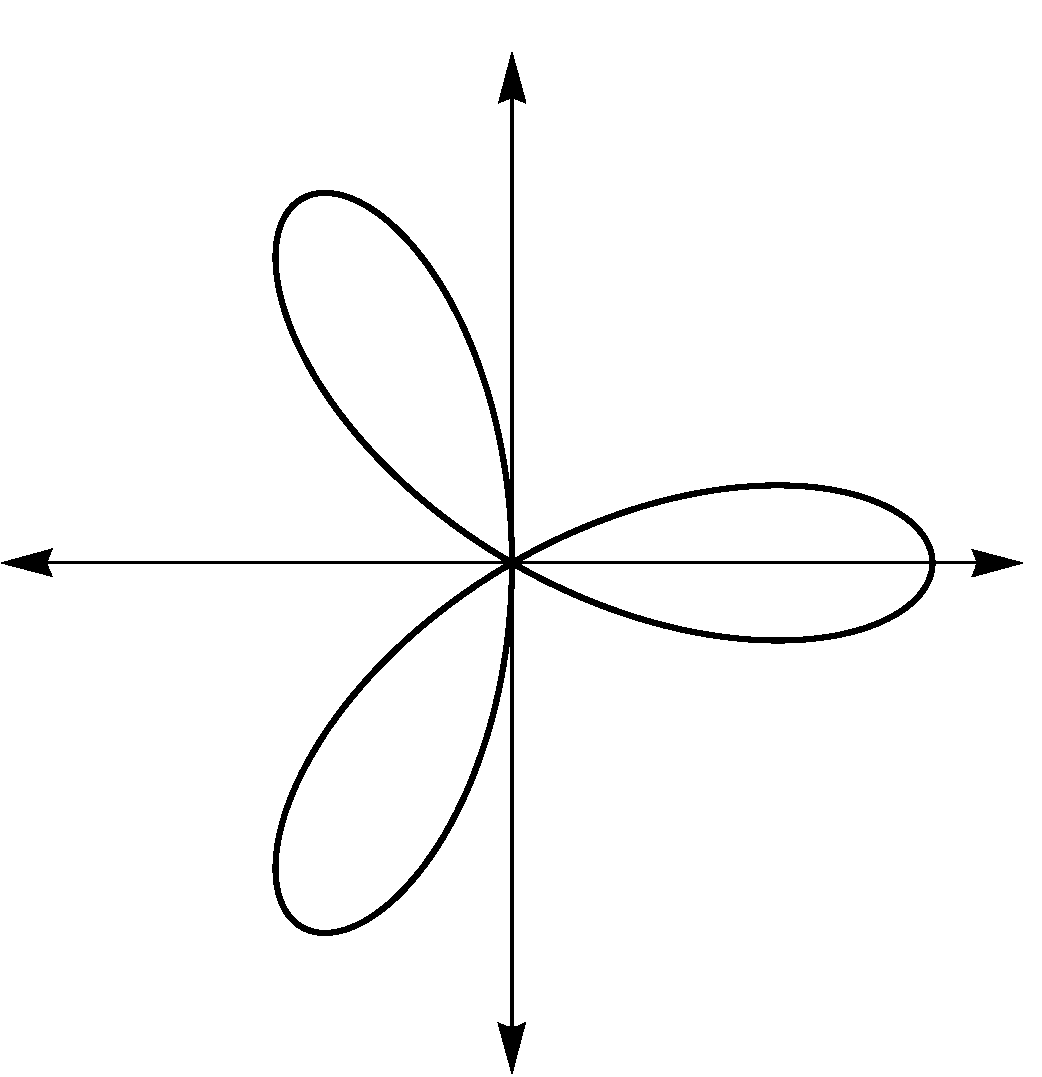
\includegraphics[width=.22\textwidth]{fig_parametric_11c} & 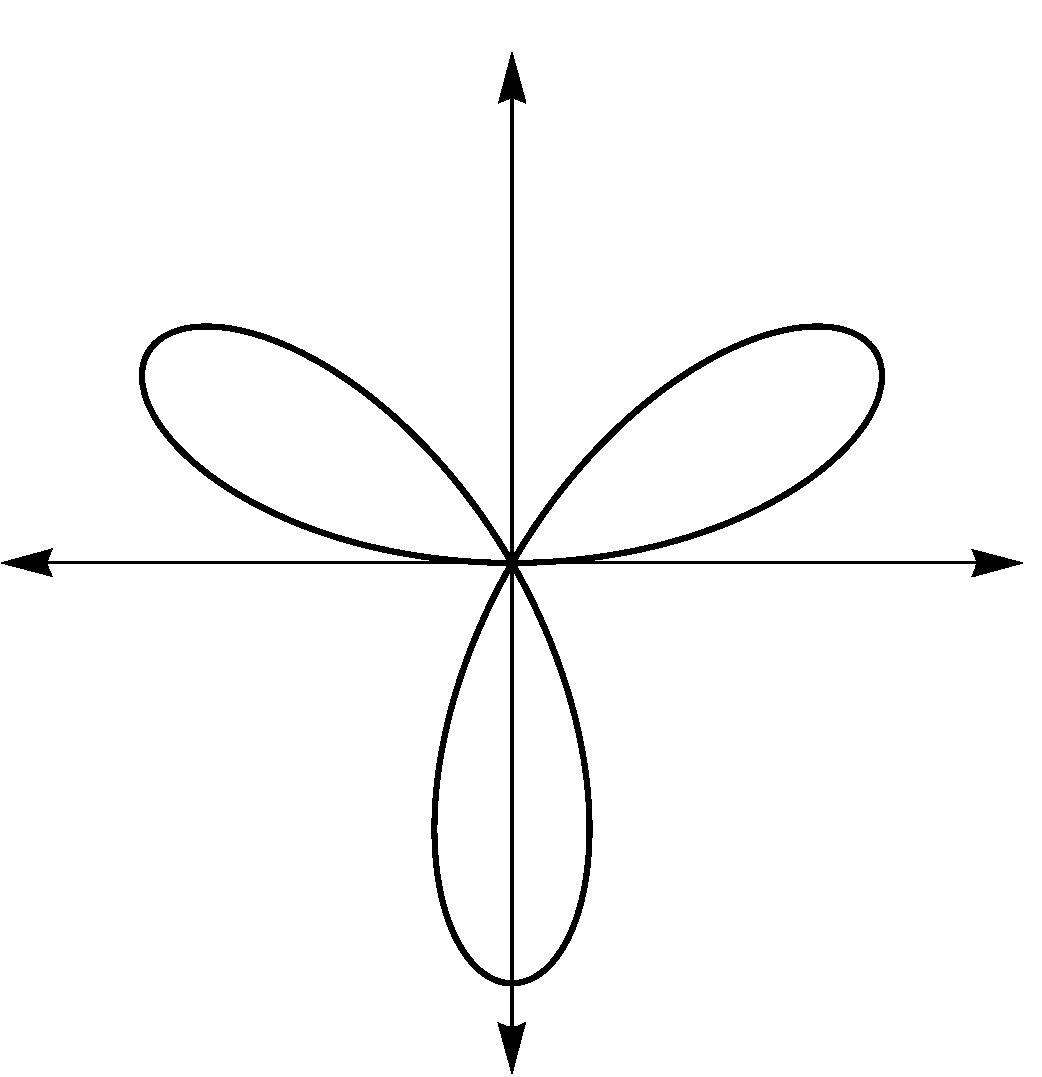
\includegraphics[width=.22\textwidth]{fig_parametric_11d}
\end{tabular}

\textbf{\large Special Curves}\\


\begin{tabular}{cccc}
\textbf{Rose curves} &  & \textbf{Lemniscate:} & \textbf{Eight Curve:} \\[5pt]
$r=a\sin (\theta/5)$ & $r=a\sin(2\theta/5)$ & $r^2=a^2\cos (2\theta)$ & $r^2=a^2\sec^4(\theta)\cos (2\theta)$ \\[10pt]
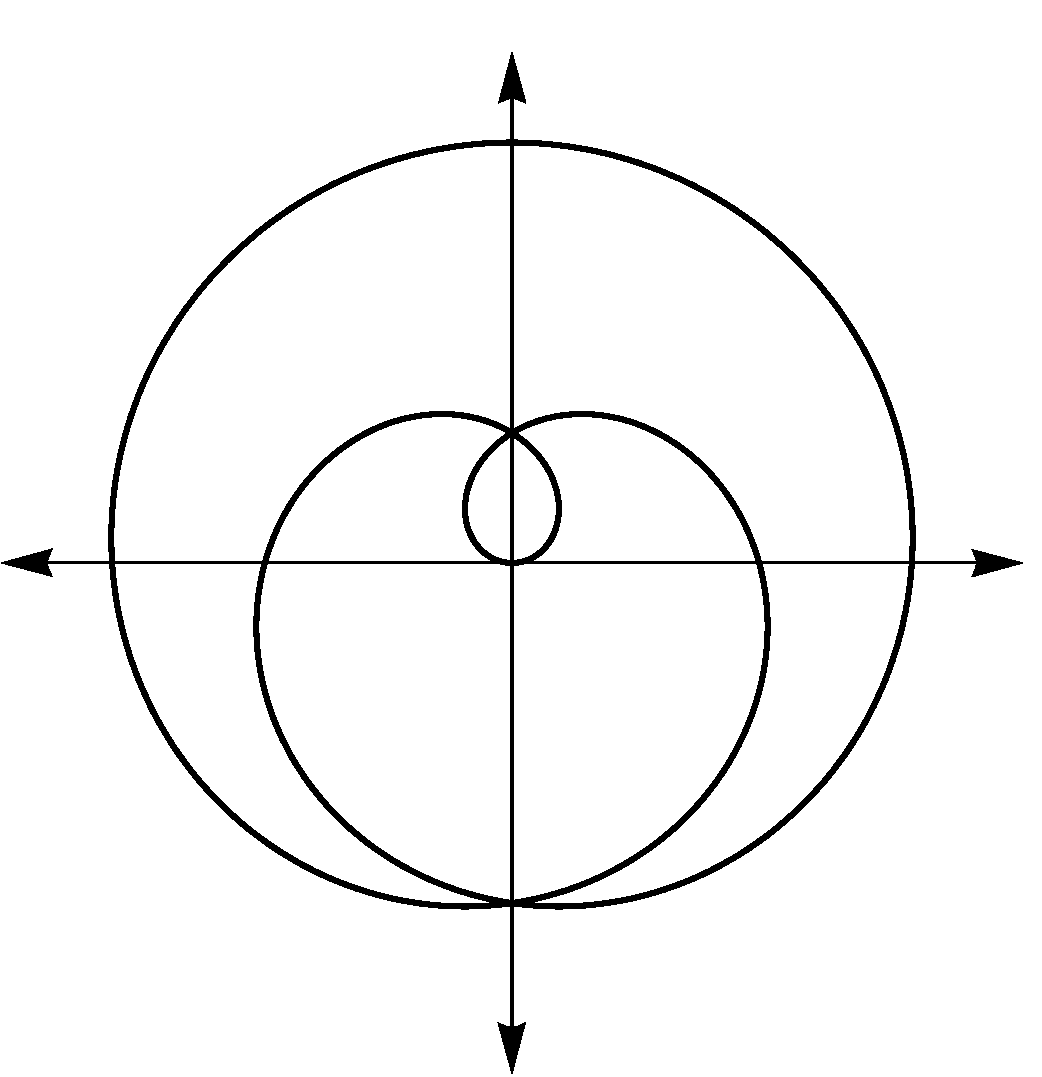
\includegraphics[width=.22\textwidth]{fig_parametric_12a} & 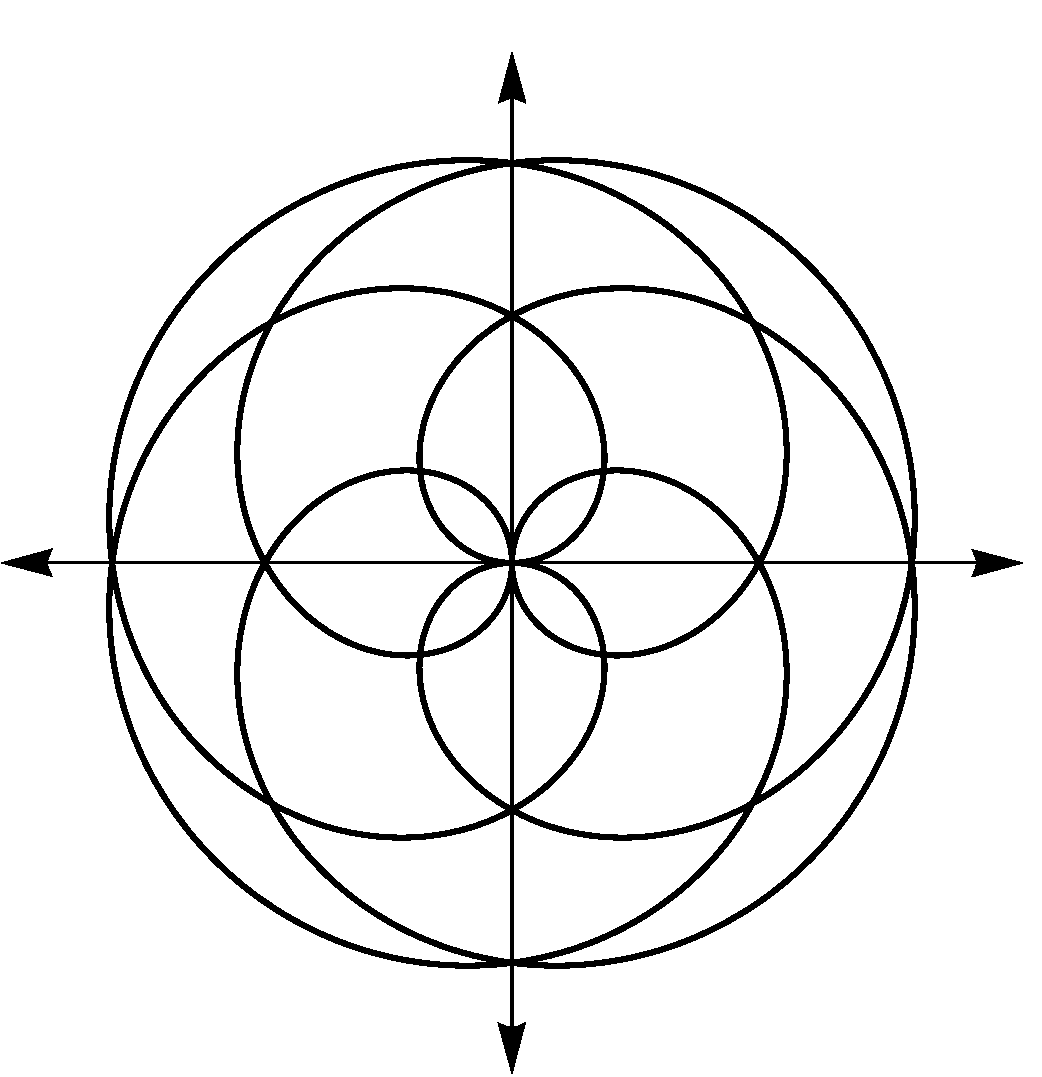
\includegraphics[width=.22\textwidth]{fig_parametric_12b} & 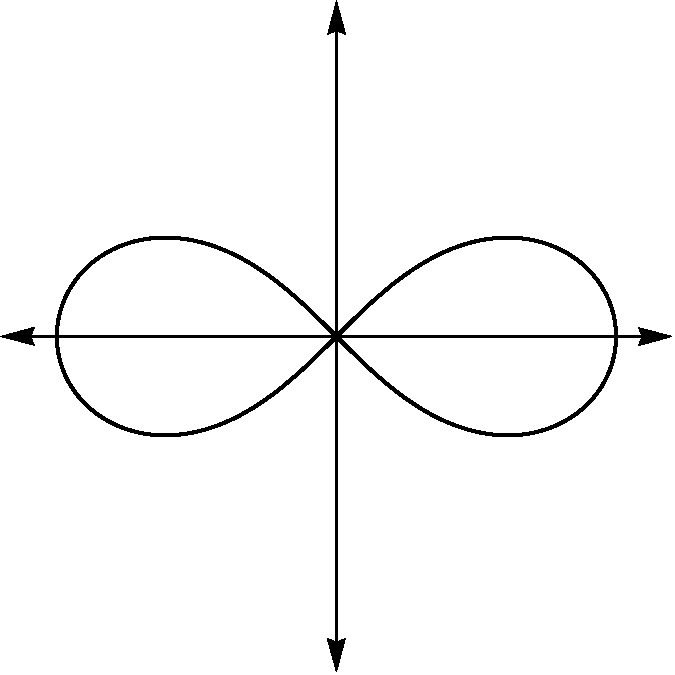
\includegraphics[width=.22\textwidth]{fig_parametric_12c} & 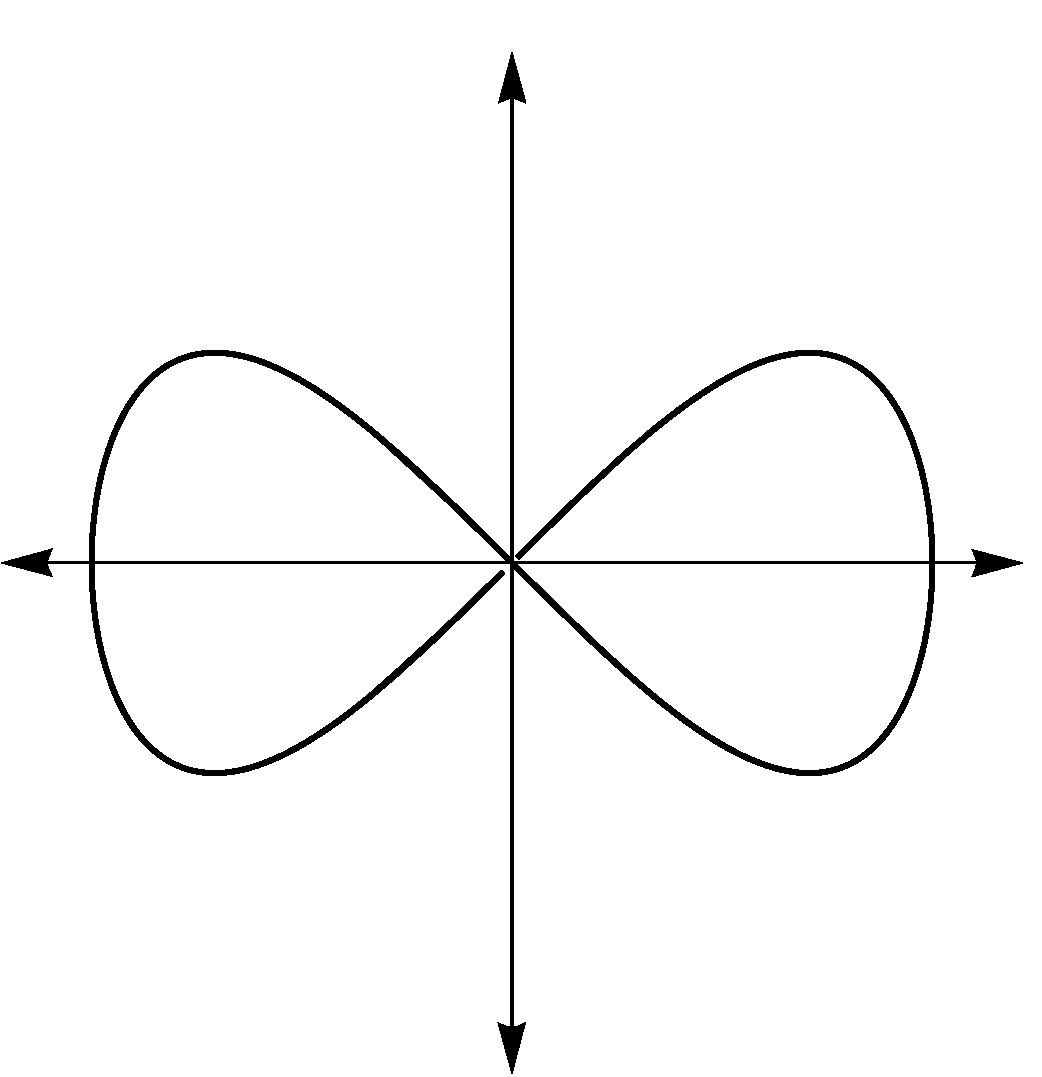
\includegraphics[width=.22\textwidth]{fig_parametric_12d}
\end{tabular}


\section{Parametric equations}
\label{sec:parameter_eq}
\subsection{Definition}
As we have seen in Section~\ref{sec_polar} there are interesting curves which, when plotted in the $xy$-plane, neither represent $y$ as a function of $x$ nor $x$ as a function of $y$.  Here, we present a new concept which allows us to use functions to study these kinds of curves.  To motivate the idea, we imagine a bug crawling across a table top starting at the point $O$ and tracing out a curve $C$ in the plane, as shown in Figure~\ref{fig_parametric_13}.

\begin{figure}
	\begin{center}
			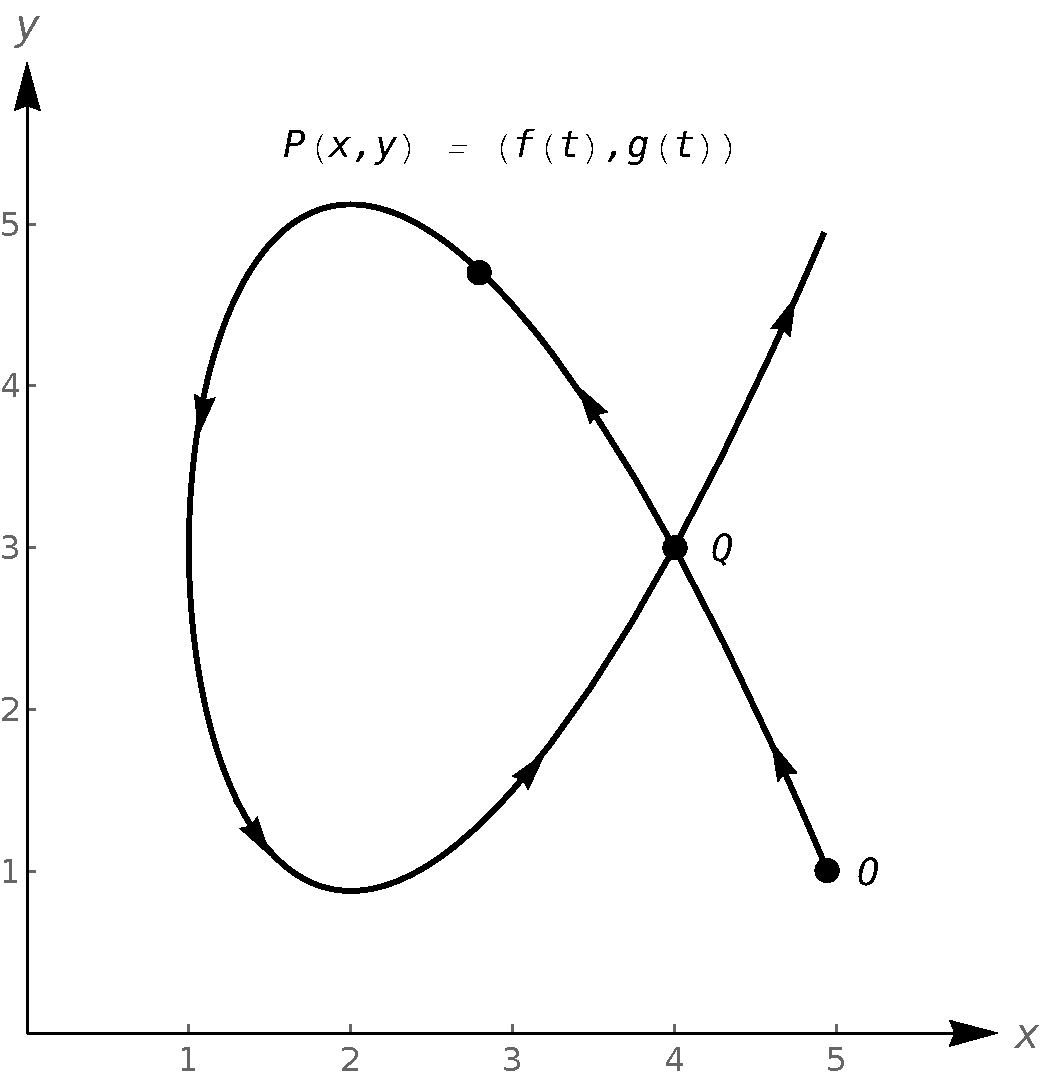
\includegraphics[width=0.4\textwidth]{fig_parametric_13}
	\caption{A bug crawling tracing out a curve $C$ in the plane. }
	\label{fig_parametric_13}
	\end{center}
\end{figure}


The curve $C$ does not represent $y$ as a function of $x$ because it fails the vertical line test and it does not represent $x$ as a function of $y$ because it fails the horizontal line test.  However, since the bug can be in only one place $P(x,y)$ at any given time $t$, we can define the $x$-coordinate of $P$ as a function of $t$ and the $y$-coordinate of $P$ as a different function of $t$.  The independent variable $t$ in this case is called a \index{parameter}\index[aut]{parameter}\textbf{parameter} (\textit{parameter}) and the system of equations 
\[ \left\{\begin{array}{rcl} x & = & f(t) \\ y & = & g(t) \\ \end{array} \right. \] 
is called a \index{parametric equations}\index[aut]{parametervergelijking}\textbf{system of parametric equations} (\textit{stelsel parametervergelijkingen}) or a \index{parametrization}\index[aut]{parametervoorstelling}\textbf{parametrization} (\textit{parametervoorstelling}) of the curve $C$.

  The parametrization of $C$ endows it with an \index{curve ! orientated} \index[aut]{zin}\index[aut]{curve ! zin}\index{orientation}\textbf{orientation} (\textit{zin}) and the arrows on $C$ indicate motion in the direction of increasing values of $t$. In this case, our bug starts at the point $O$, travels upwards to the left, then loops back around to cross its path at the point $Q$ and finally heads off into the first quadrant.   It is important to note that the curve itself is a set of points and as such is devoid of any orientation.  It is the parametrization that determines the orientation and as we shall see, different parametrizations can determine different orientations. Actually, the system of equations 
	
	\[ \left\{\begin{array}{rcl} x & = & \cos(t)\\[0.2cm] y & = & \sin(t)\\ \end{array}\right. \] 
	
	parametrizes the unit circle, giving it a counter-clockwise orientation.  More generally, the equations of circular motion (Theorem~\ref{cosinesinecircle}) 
		
	\[\left\{ \begin{array}{rcl} x & = & r\cos(\omega\,t)\\[0.2cm]
	y & = & r\sin(\omega\,t)\\ \end{array}\right. \] 
			
are parametric equations that trace out a circle of radius $r$ centred at the origin.  If $\omega > 0$, the orientation is counter-clockwise;  if $\omega < 0$, the orientation is clockwise.  The angular frequency $\omega$ determines how fast the object moves around the circle. 

\subsection{Graphing parametric equations}
Graphing parametric equations is pretty straightforward in the sense that we just choose some friendly values of $t$,  plot the corresponding points and connect the results in a pleasing fashion. For instance, consider the following system of parametric equations:

\begin{equation}
\displaystyle \left\{\begin{array}{rcl} x & =  & t^2 - 3 \\[0.2cm] y & = & 2t-1 \\ \end{array}\right.
\label{exparametric}
\end{equation}
for $t \geq -2$. 

Since we are told $t \geq -2$, we start there and evaluate $x(t)$ and $y(t)$, yielding the following values: 

\begin{center}
\renewcommand{\arraystretch}{1.5}
$\begin{array}{r|cc}  

 t & x(t) & y(t) \\ \hline\hline
-2  & 1 & -5  \\  
-1  & -2 &  -3  \\  
0 & -3 & -1  \\  
1  & -2 & 1  \\  
2 & 1 & 3  \\  
3  & 6 & 5 \\  
\end{array} $ 

\renewcommand{\arraystretch}{1}
\end{center}

Then we plot the successive points in Figure~\ref{fig_parametric_14} and we draw an arrow to indicate the direction of the path for increasing values of $t$. The curve looks like a parabola.  To verify this we may eliminate the parameter $t$ from Equation~\eqref{exparametric}.  To do so, we choose to solve the equation $y = 2t-1$ for $t$ to get $t = \frac{y+1}{2}$.  Substituting this into the equation $x = t^2 -3$ yields 
$$x = \left(\frac{y+1}{2}\right)^2 - 3$$
 or, after some rearrangement, 
\begin{equation}
(y+1)^2 = 4(x+3)\,.
\label{exparametric2}
\end{equation} 
The graph of this equation is a parabola with vertex $(-3,-1)$ which opens to the right. Technically speaking, Equation~\eqref{exparametric2} describes the entire parabola, while the parametric equations (Equation~\eqref{exparametric}) for $t \geq -2$ describe only a portion of the parabola.  In this case, we can remedy this situation by restricting the bounds on $y$.  Since the portion of the parabola we want is exactly the part where $y \geq -5$, Equation~\eqref{exparametric2} coupled with the restriction $y \geq -5$ describes the same curve as the given parametric equations.  The one piece of information we can never recover after eliminating the parameter is the orientation of the curve.


\begin{figure}[h]
	\begin{center}
			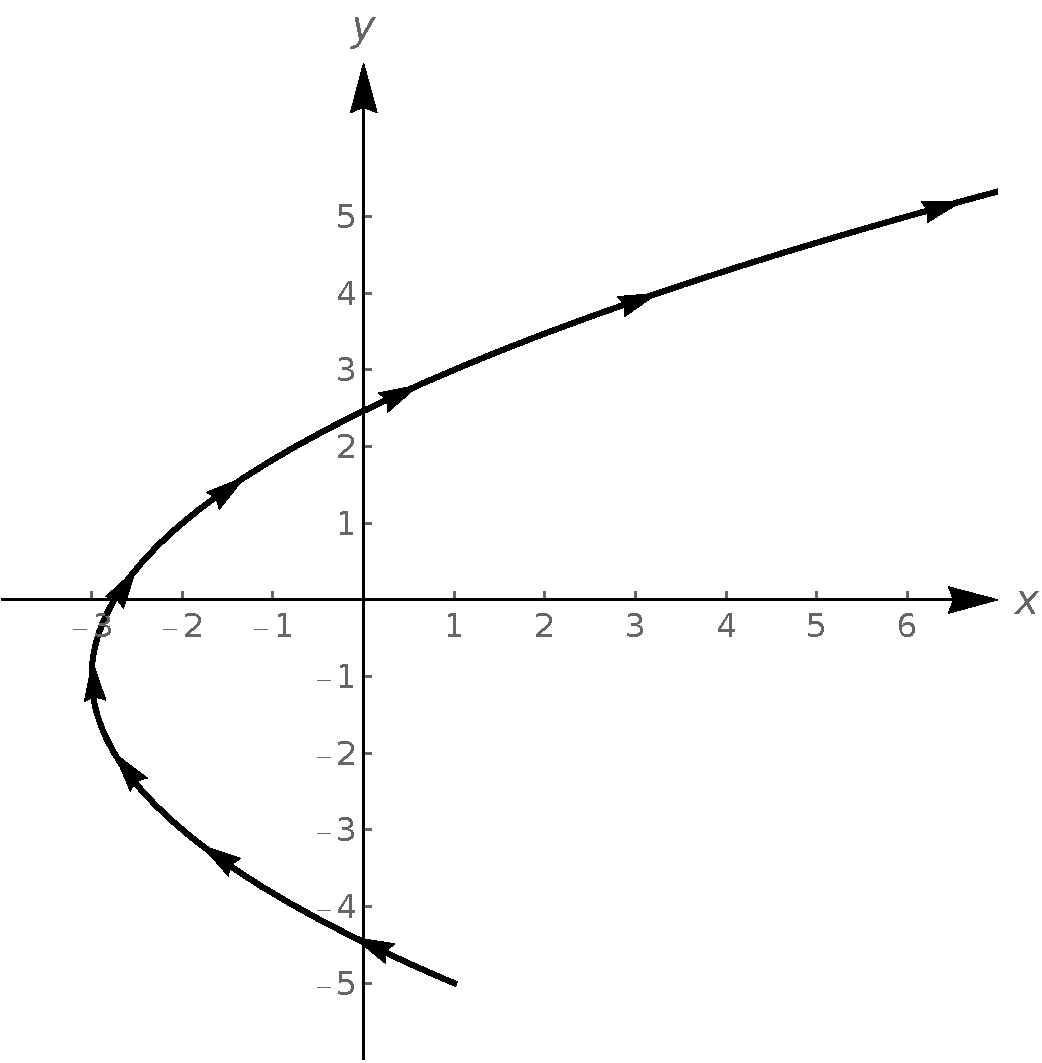
\includegraphics[width=0.4\textwidth]{fig_parametric_14}
	\caption{The curve described by Equation~\eqref{exparametric}. }
	\label{fig_parametric_14}
	\end{center}
\end{figure}

\ifmathematica
In Mathematica, we can use the built-in function \lstinline{ParametricPlot} to construct the graph of a parametric equation. For instance, for Equation~\eqref{exparametric} this can be achieved as follows. 
\begin{mdframed}[default,backgroundcolor=gray!40,roundcorner=8pt]
\begin{mmaCell}[morefunctionlocal={t},moredefined={Arrowheads}]{Input}
  ParametricPlot[\{t^2-3,2* t-1\},\{t,-2,3.2\},AxesLabel->\{"x","y"\},
	 AxesStyle->Arrowheads[\{0,0.05\}]]
\end{mmaCell}
\end{mdframed}
\fi

\ifpython
In Python, we can use the built-in function \lstinline{plot\_parametric} to construct the graph of a parametric equation. For instance, for Equation~\eqref{exparametric} this can be achieved as follows. 
\begin{pyin}
from sympy import symbols
from sympy.plotting import plot_parametric
t = symbols('t')
x = t**2 - 3
y = 2*t - 1
plot_parametric((x, y), (t, -2, 3.2), xlabel="x", ylabel="y")
\end{pyin}
\begin{pyout}
  |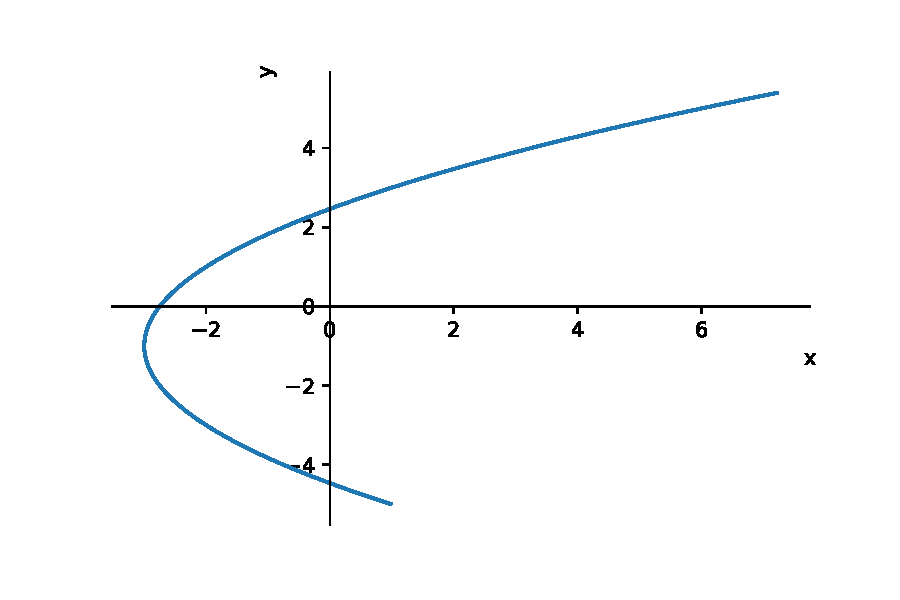
\includegraphics{figures/Parametric/fig_parametric_27_Python.pdf}|
\end{pyout}
\fi


\begin{example} \label{parametrictorect}  Sketch the curves described by the following parametric equations.  

\begin{multicols}{2}
\begin{enumerate}

\item For $-1 \leq t \leq 1$ 

$\left\{\begin{array}{rcl} x & = & t^3 \\[0.2cm] y & = & 2t^2, \end{array}\right. $


\item  \label{parametricellipse} For $0 \leq t \leq \dfrac{3\pi}{2}$
 
$ \left\{\begin{array}{rcl} x & = & 1 + 3\cos(t) \\[0.2cm] y & = & 2\sin(t), \end{array}\right. $


\end{enumerate}
\end{multicols}
\xhrulefill{gray}{2.5pt}Solution \xhrulefill{gray}{2.5pt}
\begin{enumerate}
\item  We first sketch the graphs of $x = t^3$ and $y =  2t^2$ over the interval $[-1,1]$ (Figures~\ref{fig_parametric_15a} and \ref{fig_parametric_15b}). We note that as $t$ takes on values in $[-1,1]$, $x = t^3$ ranges between $-1$ and $1$, and $y =  2t^2$ ranges between $0$ and $2$.    This means that all of the action is happening on a portion of the plane, namely $\left\{ (x,y) \, | \, -1 \leq x \leq 1, \; 0 \leq y \leq 2 \right\}$.  Next, we plot a few points.  Certainly, $t=-1$ and $t=1$ are good values to pick since these are the extreme values of $t$.  We also choose $t=0$ as this is a relative minimum on the graph of $y = 2t^2$.   Plugging in $t = -1$ gives the point $(-1,2)$, $t = 0$ gives $(0,0)$ and $t=1$ gives $(1,2)$. More generally, we see that $x = t^3$ is increasing over the entire interval $[-1,1]$ whereas $y = 2t^2$  is decreasing over the interval $[-1,0]$ and then increasing over $[0,1]$.  Geometrically, we start at $(-1,2)$ (where $t=-1$), then move to the right (since $x$ is increasing) and down (since $y$ is decreasing) to $(0,0)$ (where $t = 0$).  We continue to move to the right (since $x$ is still increasing) but now move upwards (since $y$ is now increasing) until we reach $(1,2)$ (where $t=1$).   Finally,  we eliminate the parameter.  Solving $x = t^3$ for $t$, we get $t = \sqrt[3]{x}$. Substituting this into $y = 2t^2$ gives $y = 2(\sqrt[3]{x})^2 =  2x^{2/3}$. The final graph is shown in Figure~\ref{fig_parametric_15c}.

\begin{figure}[H]
\centering
%\raisebox{0.5cm}{
\centerline{
\subfigure[\label{fig_parametric_15a}]{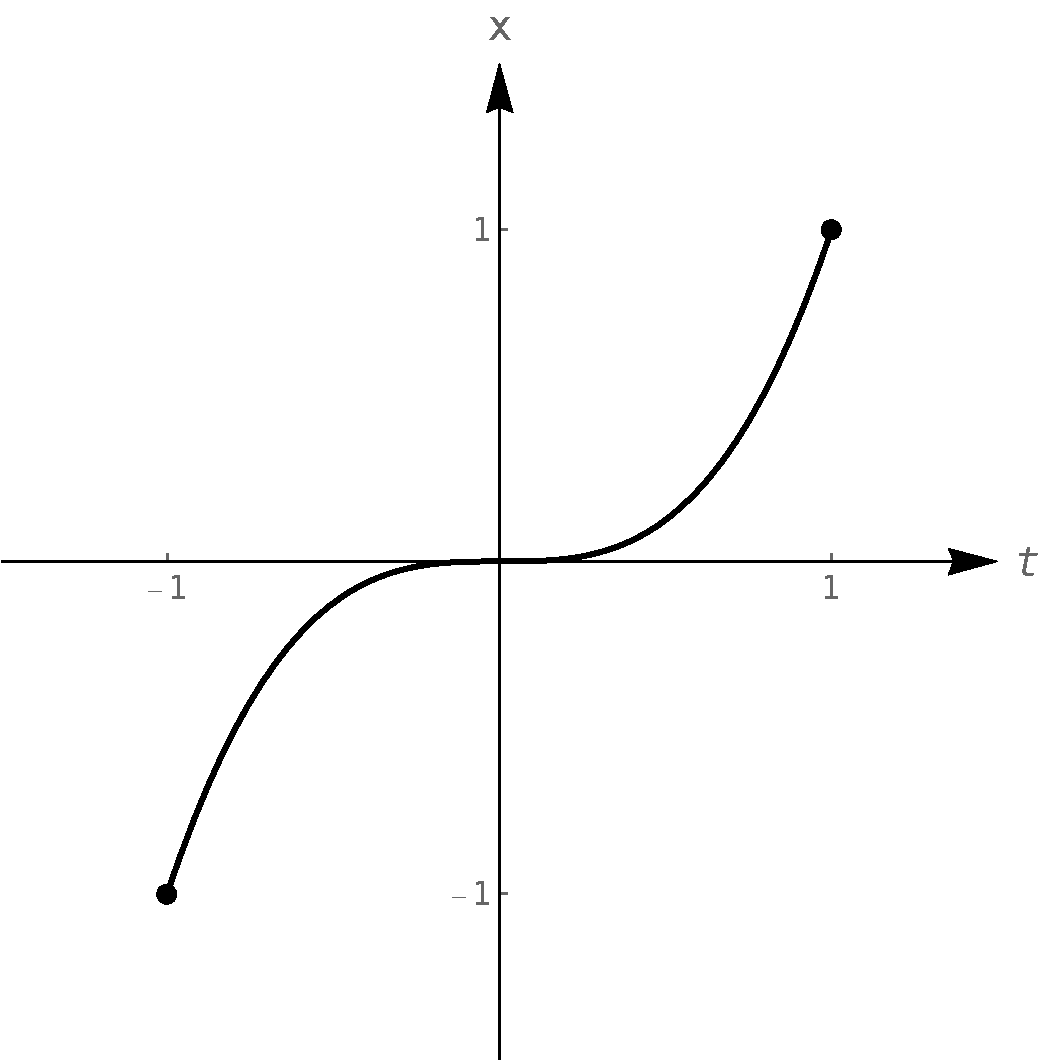
\includegraphics[width=0.33\textwidth]{fig_parametric_15a}}
\hspace{0.1cm}
\subfigure[\label{fig_parametric_15b}]{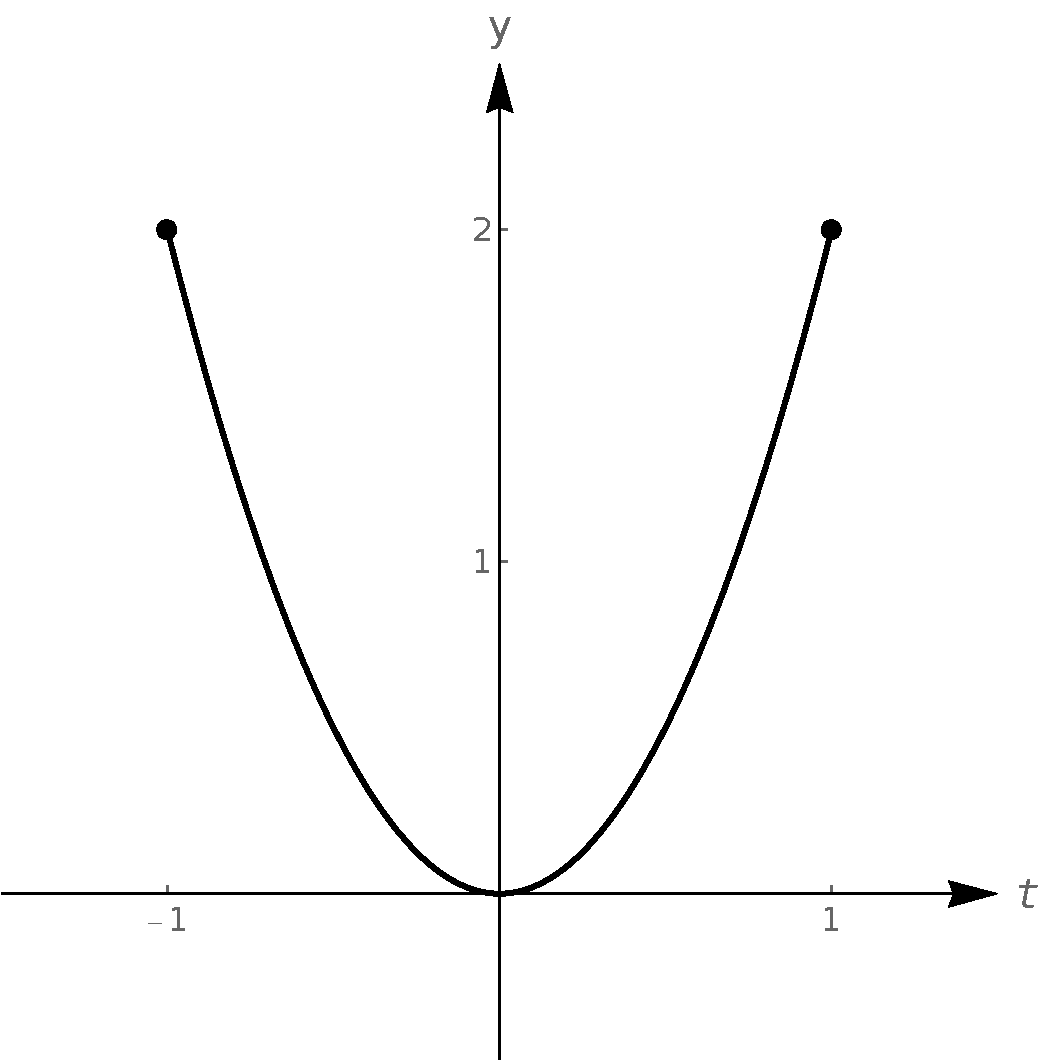
\includegraphics[width=0.33\textwidth]{fig_parametric_15b}}
\hspace{0.1cm}
\subfigure[ \label{fig_parametric_15c}]{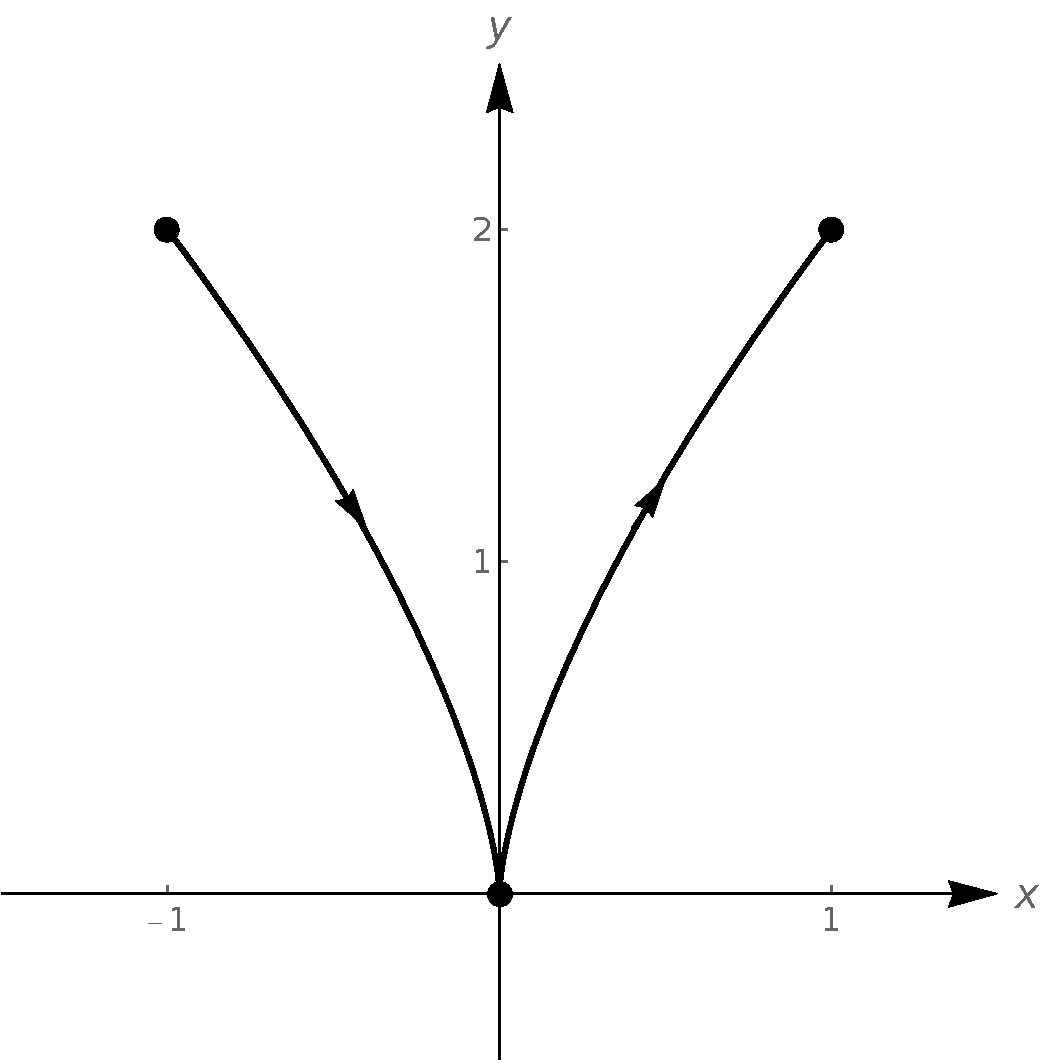
\includegraphics[width=0.33\textwidth]{fig_parametric_15c}}
}
\caption{The graph of $x=t^3$ (a), $y=2t^2$ (b) and $x=t^3$, $y=2t^2$ (c) for $-1\leq t\leq1$. }

\end{figure}

\item  Proceeding as above, we set about graphing this system by first graphing $x = 1 + 3\cos(t)$ and $y = 2\sin(t)$ on the interval $\left[0, \frac{3\pi}{2}\right]$ (Figures~\ref{fig_parametric_16a} and \ref{fig_parametric_16b}).  We see that $x$ ranges from $-2$ to $4$ and $y$ ranges from $-2$ to $2$.  Plugging in $t = 0$, $\frac{\pi}{2}$, $\pi$ and $\frac{3\pi}{2}$ gives the points $(4,0)$, $(1,2)$, $(-2,0)$ and $(1,-2)$, respectively.  As $t$ ranges from $0$ to $\frac{\pi}{2}$, $x = 1 + 3\cos(t)$ is decreasing, while $y = 2\sin(t)$ is increasing.  This means that we start tracing out our answer at $(4,0)$ and continue moving to the left and upwards towards $(1,2)$.  For $\frac{\pi}{2} \leq t \leq \pi$, $x$ is decreasing, as is $y$, so the motion is still right to left, but now is downwards from $(1,2)$ to $(-2,0)$.  On the interval $\left[\pi, \frac{3\pi}{2}\right]$, $x$ begins to increase, while $y$ continues to decrease.  Hence, the motion becomes left to right but continues downwards, connecting $(-2,0)$ to $(1,-2)$.  To eliminate the parameter here, we  use the Pythagorean identity.  Hence, we solve $x = 1+3\cos(t)$ for $\cos(t)$ to get $\cos(t) = \frac{x-1}{3}$, and we solve $y = 2\sin(t)$ for $\sin(t)$ to get $\sin(t) = \frac{y}{2}$.  Substituting these expressions into $\cos^{2}(t) + \sin^{2}(t) = 1$ gives $$\left(\frac{x-1}{3}\right)^2 + \left(\frac{y}{2}\right)^2 = 1,$$
or 
$$\frac{(x-1)^2}{9} + \frac{y^2}{4} = 1.$$
The graph of this equation is an ellipse centred at $(1,0)$ with vertices at $(-2,0)$ and $(4,0)$.  Our parametric equations here are tracing out three-quarters of this ellipse, in a  counter-clockwise direction (Figure~\ref{fig_parametric_16c}).

\begin{figure}[H]
\centering
%\raisebox{0.5cm}{
\centerline{
\subfigure[\label{fig_parametric_16a}]{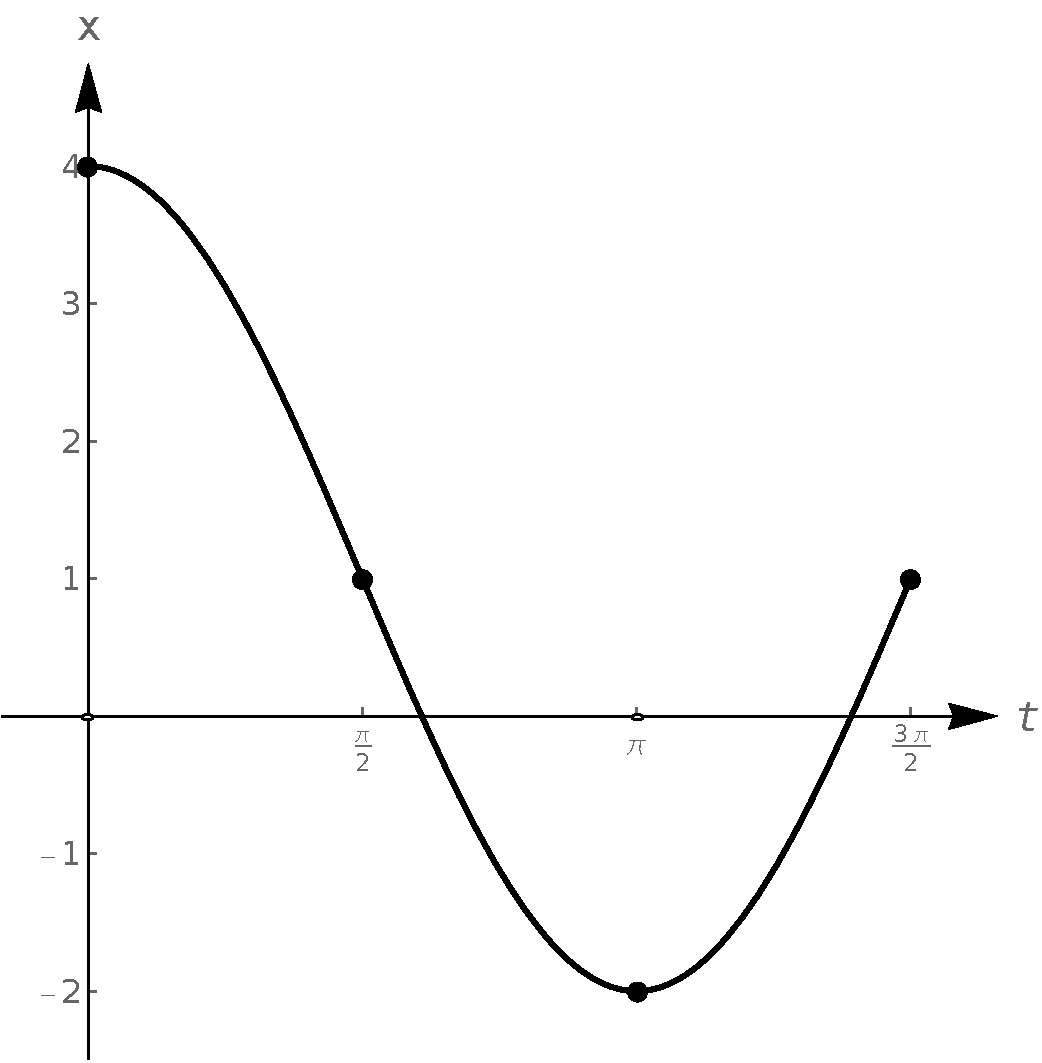
\includegraphics[width=0.33\textwidth]{fig_parametric_16a}}
\hspace{0.1cm}
\subfigure[\label{fig_parametric_16b}]{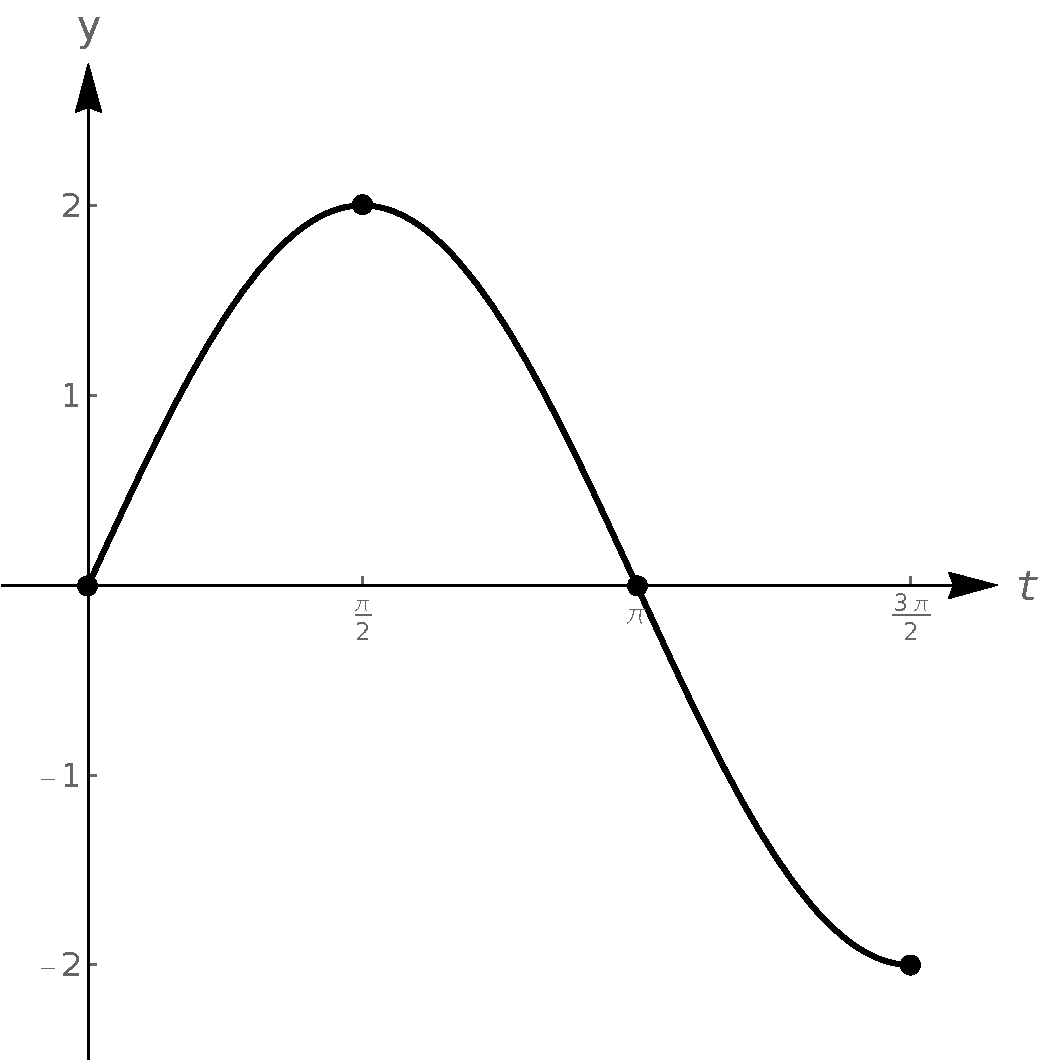
\includegraphics[width=0.33\textwidth]{fig_parametric_16b}}
\hspace{0.1cm}
\subfigure[ \label{fig_parametric_16c}]{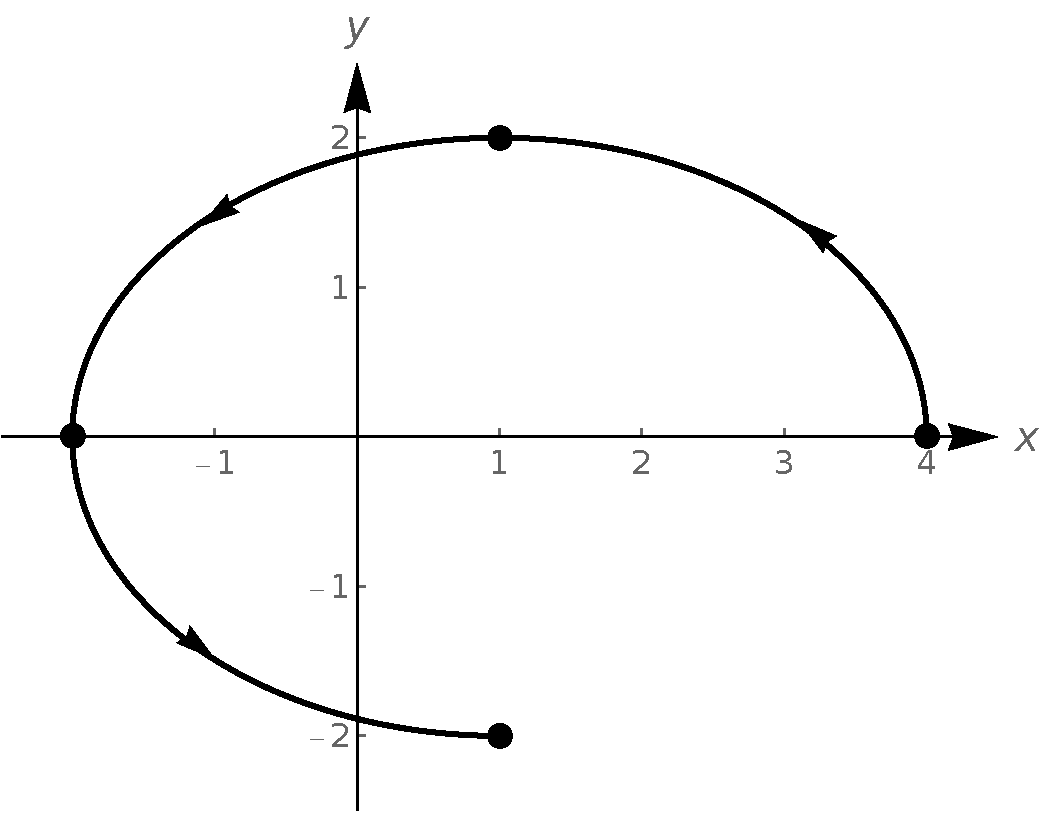
\includegraphics[width=0.33\textwidth]{fig_parametric_16c}}
}
\caption{The graph of $x=1+3\cos(t)$ (a), $y=2\sin(t)$ (b) and $x=1+3\cos(t)$, $y=2\sin(t)$ (c) for $0\leq t\leq\frac{3\pi}{2}$. }

\end{figure}

\end{enumerate}

\end{example}



\subsection{Parametrising curves}
\ifcourse
	\checkoddpage
\marginpar{\ifoddpage\hspace*{-1.5cm}\else\hspace*{0.25cm}\fi
\includegraphics[width=0.075\textwidth]{youtube}\\
\ifoddpage\hspace*{-1.75cm}\else\hspace*{0.1cm}\fi
\qrcode[height=1.75cm]{https://youtu.be/SUqm50iMOpA}
%\includegraphics[width=0.1\textwidth]{parametrising_curves}
}
 \fi
Now that we have had some good practice sketching the graphs of parametric equations, we turn to the problem of finding parametric representations of curves.  For that purpose, we have the following guidelines. 

\begin{itemize}

\item  To parametrize $y=f(x)$ as $x$ runs through some interval $I$, let $x=t$ and $y=f(t)$ and let $t$ run through $I$.

\item  To parametrize $x=g(y)$ as $y$ runs through some interval $I$, let  $y=t$ and $x=g(t)$ and  let $t$ run through $I$.

\item  To parametrize a directed line segment with initial point $(x_0, y_0)$ and terminal point $(x_1, y_1)$, let $x = x_0 + (x_1- x_0) t$ and $y = y_0 + (y_1 - y_0) t$ for $0 \leq t \leq 1$.

\item  To parametrize  $\frac{(x-x_0)^2}{a^2} + \frac{(y-y_0)^2}{b^2} = 1$ where $a,b > 0$, let $x = x_0+a\cos(t)$ and $y=y_0+b\sin(t)$ for $0 \leq t < 2\pi$.  This will impart a counter-clockwise orientation.

\end{itemize}


\begin{example} \label{recttoparametric}  Find a parametrization for each of the following curves.

\begin{enumerate}

\item $y = x^2$ from $x = -3$ to $x = 2$.

\item  The line segment which starts at $(2,-3)$ and ends at $(1,5)$.

\item  The circle $x^2 + 2x + y^2 - 4y = 4$.

\item  The left half of the ellipse 
$$\frac{x^2}{4} + \frac{y^2}{9} = 1.$$

\end{enumerate}

\xhrulefill{gray}{2.5pt}Solution \xhrulefill{gray}{2.5pt}

\begin{enumerate}

\item  Since $y = x^2$ is written in the form $y = f(x)$, we let $x = t$ and $y = f(t) = t^2$.  Since $x=t$, the bounds on $t$ match precisely the bounds on $x$ so we get 
$$
\left\{\begin{array}{rcl} x & = & t \\[0.2cm] y & = & t^2, \end{array}\right.
$$
for $-3 \leq t \leq 2$.

\item   To find the equation for $x$, we have that the line segment starts at $x= 2$ and ends at $x = 1$.  This means the displacement in the $x$-direction is $(1-2) = -1$.  Hence, the equation for $x$ is $x = 2 + (-1)t = 2-t$.  For $y$, we note that the line segment starts at $y=-3$ and ends at $y=5$.  Hence, the displacement in the $y$-direction is $(5-(-3)) = 8$, so we get $y = -3+8t$.  Our final answer is
$$
\left\{\begin{array}{rcl} x & = & 2-t \\[0.2cm] y & = & -3+8t, \end{array}\right.
$$
for $0 \leq t \leq 1$.

\item In order to use the formulas above to parametrize the circle $x^2 + 2x + y^2 - 4y = 4$, we first need to put it into the correct form.  We complete the square and get $(x+1)^2+(y-2)^2 = 9$, or 
$$\frac{(x+1)^2}{9} + \frac{(y-2)^2}{9} = 1.$$
In this equation, we identify $\cos(t) = \frac{x+1}{3}$ and $\sin(t) = \frac{y-2}{3}$.  Rearranging these last two equations, we get $x = -1+3 \cos(t)$ and $y = 2 +3 \sin(t)$.   In order to complete one revolution around the circle, we let $t$ range through the interval $[0,2\pi\left[\right.$.  We get as our final answer
$$  
\left\{\begin{array}{rcl} x & = & -1+3 \cos(t)\\[0.2cm] y & = & 2 +3 \sin(t), \end{array}\right.
$$
for $0 \leq t < 2\pi$.

\item  We immediately get  $x = 2\cos(t)$ and $y = 3\sin(t)$.  The normal range on the parameter in this case is $0 \leq t < 2\pi$, but since we are interested in only the left half of the ellipse, we restrict $t$ to the values which correspond to Quadrant II and Quadrant III angles, namely  $\frac{\pi}{2} \leq t \leq \frac{3\pi}{2}$.   Our final answer is 
$$
\left\{\begin{array}{rcl} x & = & 2 \cos(t)\\ y & = & 3 \sin(t), \end{array}\right.
$$ 

for $\frac{\pi}{2} \leq t \leq \frac{3\pi}{2}$. 
\end{enumerate}
\end{example}


We note that the parametrisation approach offers only one of literally infinitely many ways to parametrize the concerning curves. Essentially, there are two easy ways to alter parametrizations.

\begin{itemize}

\item  \textbf{Reversing Orientation:}  Replacing every occurrence of $t$ with $-t$ in a parametric description for a curve reverses the orientation of the curve.  

\item  \textbf{Shift of Parameter:}  Replacing every occurrence of $t$ with $(t-c)$ in a parametric description for a curve shifts the start of the parameter $t$ ahead by $c$ units.

\end{itemize}

These techniques are illustrated in the following example.

\begin{example} \label{adjustparametricex}  
Find a parametrization for the unit circle, oriented clockwise, with $t=0$ corresponding to $(0,-1)$.


\xhrulefill{gray}{2.5pt}Solution \xhrulefill{gray}{2.5pt}

We know that 
$$
\left\{\begin{array}{rcl} x & = & \cos(t)\\[0.2cm] y & = & \sin(t), \end{array}\right.
$$
for $0 \leq t < 2\pi$ gives a counter-clockwise parametrization of the unit circle with $t = 0$ corresponding to $(1,0)$, so the first order of business is to reverse the orientation.  Replacing $t$ with $-t$ gives 
$$
\left\{\begin{array}{rcl} x & = & \cos(-t)\\[0.2cm] y & = & \sin(-t), \end{array}\right.\,
$$
for $0 \leq t < 2\pi$
which simplifies to
$$
\left\{\begin{array}{rcl} x & = & \cos(t)\\[0.2cm] y & = & -\sin(t), \end{array}\right.\,
$$
for $0 \leq t < 2\pi$. 

 This parametrization gives a clockwise orientation, but $t=0$ still corresponds to the point $(1,0)$; the point $(0, -1)$ is reached when $t = -\frac{3\pi}{2}$.  Our strategy is to first get the parametrization to start at the point $(0,-1)$ and then shift the parameter accordingly so the start coincides with $t = 0$.  We know that any interval of length $2\pi$ will parametrize the entire circle, so we start the parameter $t$ at $-\frac{3\pi}{2}$, and find the upper bound by adding $2\pi$ so $-\frac{3\pi}{2} \leq t < \frac{\pi}{2}$.   We now shift the parameter by introducing a time delay of $\frac{3\pi}{2}$ units by replacing every occurrence of $t$ with $\left(t - \frac{3\pi}{2}\right)$, i.e.
$$
\left\{\begin{array}{rcl} x & = & \cos\left(t - \frac{3\pi}{2}\right)\\[0.2cm] y & = & -\sin\left(t - \frac{3\pi}{2}\right), \end{array}\right.\,
$$
 for  $-\frac{3\pi}{2} \leq t - \frac{3\pi}{2} < \frac{\pi}{2}$.  This simplifies to 
\begin{equation}
\left\{\begin{array}{rcl} x & = & -\sin(t)\\ y & = & -\cos(t), \end{array}\right.\,
\label{cycloide1}
\end{equation}
 for $ 0 \leq t  < 2\pi$, as required.


\end{example}

\ifanalysis

We can now use our answer to Example~\ref{adjustparametricex} to derive the equation of a \index{cycloid}\index[aut]{cyclo\"ide}\textbf{cycloid} (\textit{cyclo\"ide}).  Suppose a circle of radius $r$ rolls along the positive $x$-axis at a constant velocity $v$ as pictured in Figure~\ref{fig_parametric_17}.  Let $\theta$ be the angle in radians which measures the amount of clockwise rotation experienced by the radius highlighted in the figure.  

Our goal is to find parametric equations for the coordinates of the point $P(x,y)$ in terms of $\theta$.  From  Example \ref{adjustparametricex}, we know that clockwise motion along the unit circle starting at the point $(0,-1)$ can be modelled by Equation~\eqref{cycloide1} . To model this motion on a circle of radius $r$, all we need to do is multiply both $x$ and $y$ by the factor $r$ which yields 
$$
\left\{\begin{array}{rcl} x & = & -r\sin(\theta)\\[0.2cm] y & = & -r\cos(\theta). \end{array}\right.\,
$$  
We now need to adjust for the fact that the circle is not stationary with centre $(0,0)$, but rather, is rolling along the positive $x$-axis.  Since the velocity $v$ is constant, we know that at time $t$, the centre of the circle has travelled a distance $vt$ down the positive $x$-axis.  Furthermore, since the radius of the circle is $r$ and the circle is not  moving vertically, we know that the centre of the circle is always $r$ units above the $x$-axis.  Putting these two facts together, we have that at time $t$, the centre of the circle is at the point $(vt,r)$. We know from Chapter~\ref{chap_trans} that $v = \frac{r \theta}{t}$, or $vt = r\theta$.  Hence, the centre of the circle, in terms of the parameter $\theta$, is $(r\theta,r)$. As a result, we need to modify the governing equations by shifting the $x$-coordinate to the right $r\theta$ units and the $y$-coordinate up $r$ units.  In this way, we get 
$$
\left\{\begin{array}{rcl} x & = &  -r\sin(\theta)+ r\theta\\[0.2cm] y & = & -r\cos(\theta) + r, \end{array}\right.\,
$$
which can be written as 
$$
\left\{\begin{array}{rcl} x & = &  r(\theta -\sin(\theta))\\[0.2cm] y & = & r(1-\cos(\theta)). \end{array}\right.\,
$$
 Since the motion starts at $\theta = 0$ and proceeds indefinitely, we set  $\theta \geq 0$.  


\begin{figure}
	\begin{center}
			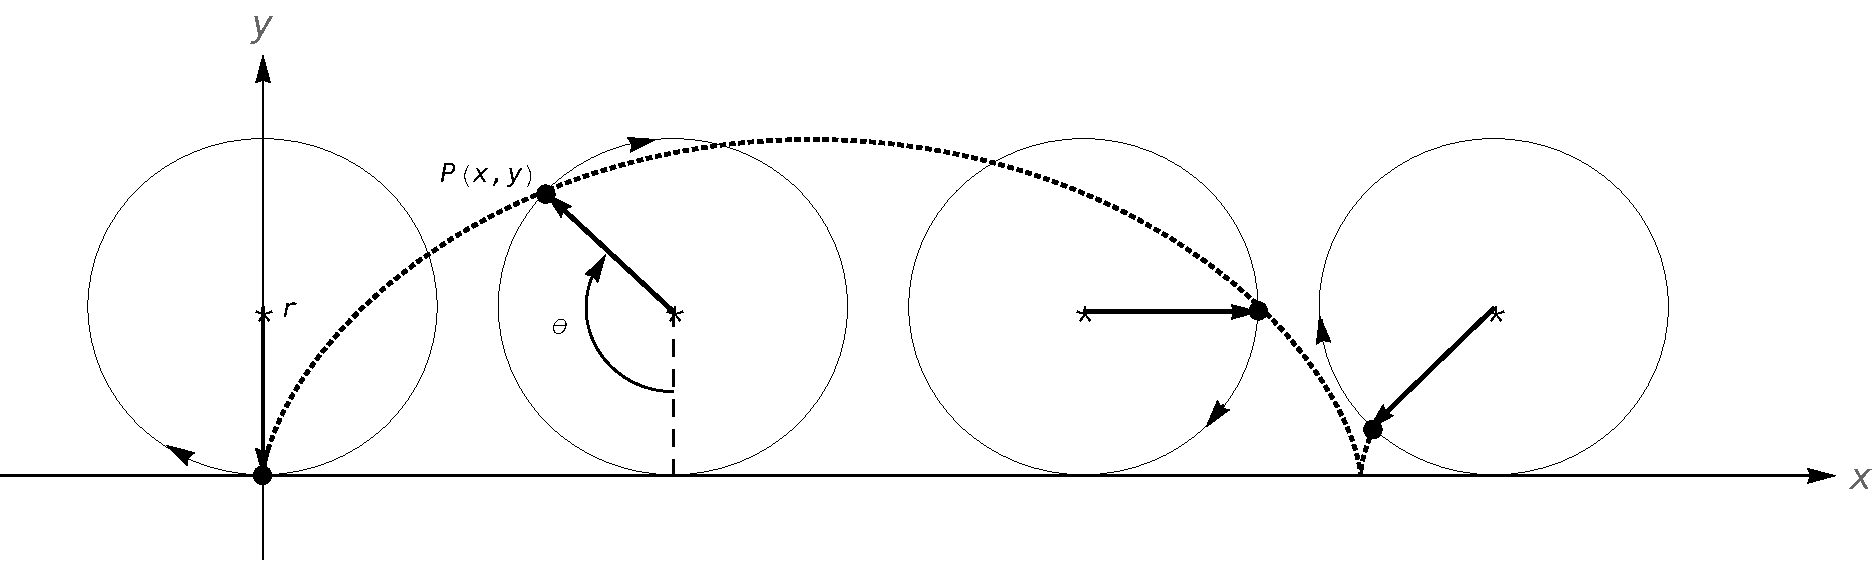
\includegraphics[width=0.75\textwidth]{fig_parametric_17}
	\caption{Constructing a cycloid from a rolling circle with radius $r$. }
	\label{fig_parametric_17}
	\end{center}
\end{figure}



\fi

Figure~\ref{fig_parametric_18} gives a small gallery of interesting and famous curves along with the parametric equations that produce them. 


\begin{figure}[t]
	\begin{center}
\begin{tabular}{cc}
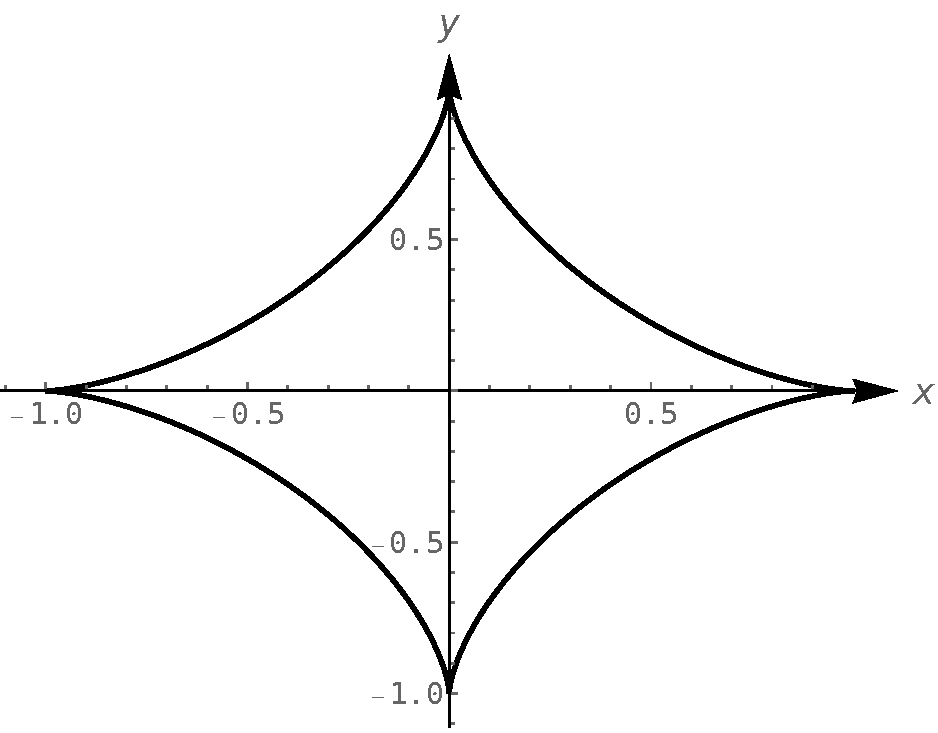
\includegraphics[width=0.45\textwidth]{fig_parametric_18a} &  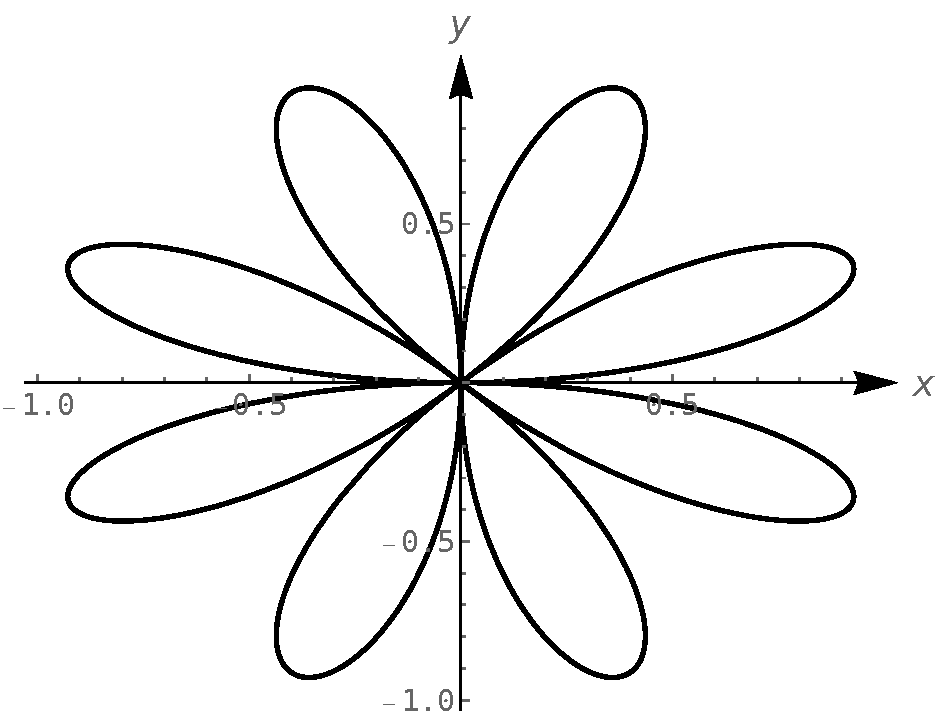
\includegraphics[width=0.45\textwidth]{fig_parametric_18b}\\


\parbox{150pt}{\centering Astroid\\ $x=\cos^3 (t)$\\ $y=\sin^3(t)$} & \parbox{150pt}{\centering Rose Curve\\ $x=\cos(t)\sin(4t)$\\ $y=\sin(t)\sin(4t)$}\\ 
\ifanalysis
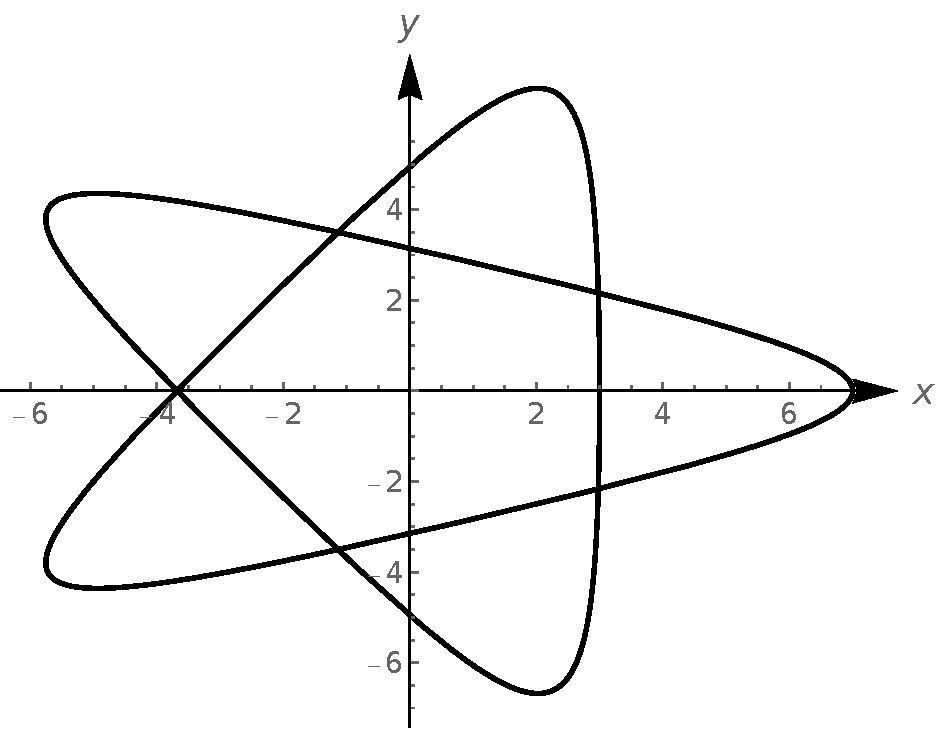
\includegraphics[width=0.45\textwidth]{fig_parametric_18c} & 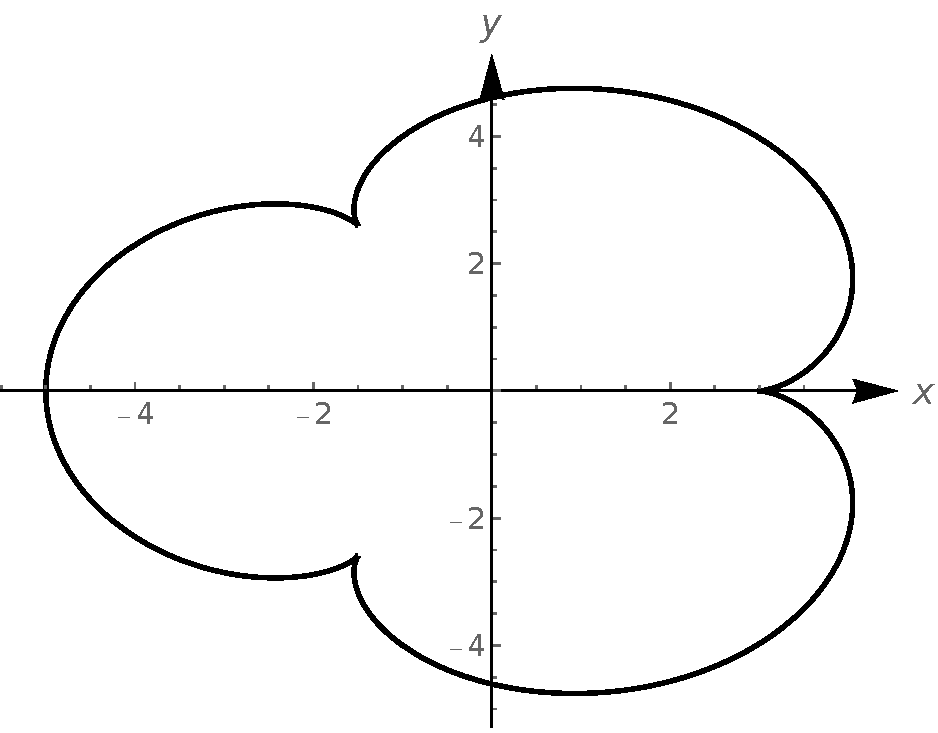
\includegraphics[width=0.45\textwidth]{fig_parametric_18d}\\
\parbox{150pt}{\centering Hypotrochoid\\ $x=2\cos(t)+5\cos(2t/3)$\\$y=2\sin(t)-5\sin(2t/3)$} & \parbox{150pt}{\centering Epicycloid\\ $x=4\cos(t)-\cos(4t)$\\$y=4\sin(t)-\sin(4t)$}
\fi
\end{tabular}		
	\caption{A gallery of interesting planar curves. }
	\label{fig_parametric_18}
	\end{center}
\end{figure}

\subsection{Conic sections continued even further}
For completeness, we conclude this chapter by listing the parametric representations of the conic sections we introduced in Section~\ref{sec_conic}. 

The parametric representation of a circle with centre at the origin and radius $r$ is given by
\begin{equation}
 \left\{\begin{array}{l}
x = r \cos(t) \\ [0.2cm]
y = r \sin(t), 
 \end{array} \right.\,
\end{equation}
for $0 \leq t \leq 2 \pi$. Likewise, the parametric representation of an ellipse centred at the origin and with semi-major and conjugate axis of $a$ and $b$ respectively ($a>b$), is given by
\begin{equation}
\left\{\begin{array}{l}
x = a \cos(t) \\ [0.2cm]
y = b \sin(t),
\end{array} \right.\,
\end{equation}
for $0 \leq t \leq 2 \pi$. 

% For what concerns a horizontal hyperbola centred at the origin with semi-major and conjugate axis of $a$ and $b$ respectively, we have the following parametric equation
% \begin{equation}
% \left\{	\begin{array}{l}
% x = a \sec (t) \\ [0.2cm]
% y = \pm b \tan(t), 
% \end{array} \right.\,
% \end{equation}
% for $0 \leq t \leq 2 \pi$, but $t\neq\frac{\pi}{2}$ and $t\neq\frac{3\pi}{2}$.


% \ifanalysis
% 
% An alternative parametric representation of such a hyperbola uses hyperbolic functions:
% \begin{equation}
% 	\left\{\begin{array}{l}
% x = \pm a \cosh (t) \\ [0.2cm]
% y = b \sinh(t),
% \end{array} \right.\,
% \end{equation}
% for $t\in\mathbb{R}$.
% 
% \fi



\section{Derivatives and parametric and polar equations}
\label{sec:deriv_par_polar_eq}
\subsection{Parametric equations}

 \ifcourse
 	\checkoddpage
\marginpar{\ifoddpage\hspace*{-1.5cm}\else\hspace*{0.25cm}\fi
\includegraphics[width=0.075\textwidth]{youtube}\\
\ifoddpage\hspace*{-1.75cm}\else\hspace*{0.1cm}\fi
\qrcode[height=1.75cm]{https://youtu.be/AXasQLqazWU}
%\includegraphics[width=0.1\textwidth]{diff_para_vgln}
}
 \fi
Here we will exemplify the techniques of calculus to study curves given by a set of parametric equations. Amongst other things, we are interested in lines tangent to points on such a curve. They describe how the $y$-values are changing with respect to the $x$-values, they are useful in making approximations, and they indicate instantaneous direction of travel.

The slope of the tangent line is still $\frac{dy}{dx}$, and the chain rule allows us to calculate this in the context of parametric equations. If $x=f(t)$ and $y=g(t)$, the chain rule states that $$\frac{dy}{dt} = \frac{dy}{dx}\,\frac{dx}{dt}\,.$$
Solving for $\frac{dy}{dx}$, we get 
\begin{equation}
\frac{dy}{dx} = \dfrac{\quad\dfrac{dy}{dt}\quad}{\dfrac{dx}{dt}} = \frac{g'(t)}{\fp(t)},
\label{idea:dydxpar}
\end{equation}
provided that $\fp(t)\neq 0$, and we also assume that $f$ and $g$ are differentiable on some open interval $I$. 

These pieces of information allow us to define the tangent and normal lines to a curve $C$.

\begin{definition}[Tangent and normal lines]\label{def:tangent_par}
Let a curve $C$ be parametrized by $x=f(t)$ and $y=g(t)$, where $f$ and $g$ are differentiable functions on some interval $I$ containing $t=t_0$. The \textbf{tangent line} to $C$ at $t=t_0$ is the line through $\big(f(t_0),g(t_0)\big)$ with slope $$m=\dfrac{g'(t_0)}{\fp(t_0)},$$
provided $\fp(t_0)\neq 0$.\\

The \textbf{normal line} to $C$ at $t=t_0$ is the line through $\big(f(t_0),g(t_0)\big)$ with slope $m=-\fp(t_0)/g'(t_0)$, provided $g'(t_0)\neq 0$.\index{tangent line}\index{normal line}\index[aut]{raaklijn}\index[aut]{normaal}
\end{definition}

This definition leaves two special cases to consider. When the tangent line is horizontal, the normal line is undefined by the above definition as $g'(t_0)=0$. Likewise, when the normal line is horizontal, the tangent line is undefined. It seems reasonable that these lines be defined, so we add the following to the above definition.

	
\begin{enumerate}
	\item If the tangent line at $t=t_0$ has a slope of 0, the normal line to $C$ at $t=t_0$ is the line $x=f(t_0)$.
	\item		If the normal line at $t=t_0$ has a slope of 0, the tangent line to $C$ at $t=t_0$ is the line $x=f(t_0)$.
	\end{enumerate}

\begin{example}\label{ex_parcalc1}
Let $x=5t^2-6t+4$ and $y=t^2+6t-1$, and let $C$ be the curve defined by these equations.
\begin{enumerate}
	\item Find the equations of the tangent and normal lines to $C$ at $t=3$.
	\item	Find where $C$ has vertical and horizontal tangent lines.
\end{enumerate}

\xhrulefill{gray}{2.5pt}Solution \xhrulefill{gray}{2.5pt}

\begin{enumerate}
		\item We start by computing $\fp(t) = 10t-6$ and $g'(t) =2t+6$. Thus $$\frac{dy}{dx} = \frac{2t+6}{10t-6}.$$
		Make note of something that might seem unusual: $\frac{dy}{dx}$ is a function of $t$, not $x$. Just as points on the curve are found in terms of $t$, so are the slopes of the tangent lines.
		
		The point on $C$ at $t=3$ is $(31,26)$. The slope of the tangent line is $m=1/2$ and the slope of the normal line is $m=-2$. Thus,
		\begin{itemize}
			\item the equation of the tangent line is $y=\frac12(x-31)+26$, and
			\item	the equation of the normal line is $\ds y=-2(x-31)+26$.
		\end{itemize}
		This is illustrated in Figure \ref{fig_parametric_19}.
		
				\begin{figure}[H]
	\begin{center}
			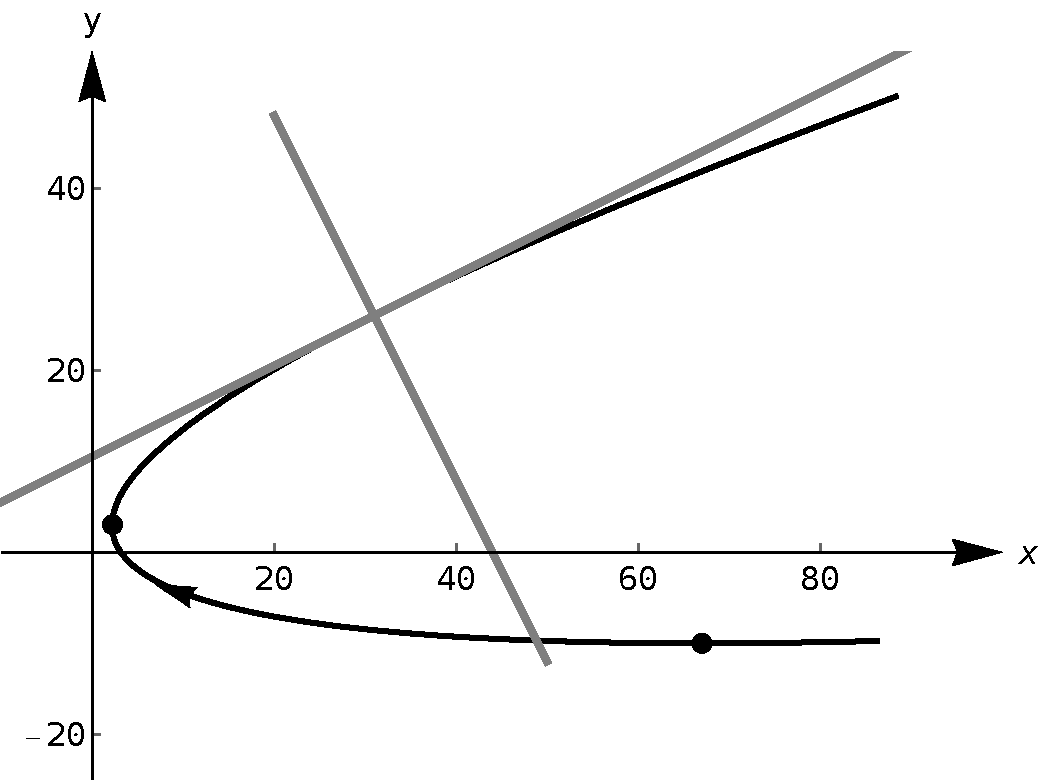
\includegraphics[width=0.5\textwidth]{fig_parametric_19}
	\caption{Graphing tangent and normal lines in Example \ref{ex_parcalc1}.}
	\label{fig_parametric_19}
	\end{center}
\end{figure}
		
		\item		To find where $C$ has a horizontal tangent line, we set $\frac{dy}{dx}=0$ and solve for $t$. In this case, this amounts to setting $g'(t)=0$ and solving for $t$ (and making sure that $\fp(t)\neq 0$): 
		$$g'(t)=0 \quad \Rightarrow \quad 2t+6=0 \quad \Leftrightarrow \quad t=-3.$$
		The point on $C$ corresponding to $t=-3$ is $(67,-10)$; the tangent line at that point is horizontal (hence with equation $y=-10$).
		
		To find where $C$ has a vertical tangent line, we find where it has a horizontal normal line, and set $-\frac{\fp(t)}{g'(t)}=0$. This amounts to setting $\fp(t)=0$ and solving for $t$ and making sure that $g'(t)\neq 0$. 
		$$\fp(t)=0 \quad \Rightarrow \quad 10t-6=0 \quad \Leftrightarrow \quad t=0.6.$$
		The point on $C$ corresponding to $t=0.6$ is $(2.2,2.96)$. The tangent line at that point is $x=2.2$.
	
		\end{enumerate}
		


\end{example}

\begin{example}\label{ex_parcalc3}
Find the equation of the tangent line to the astroid $x=\cos^3 (t)$, $y=\sin^3(t)$ at $t=0$ shown in Figure~\ref{fig_parametric_18}.

\xhrulefill{gray}{2.5pt}Solution \xhrulefill{gray}{2.5pt}

We start by finding $x'(t)$ and $y'(t)$:
$$ x'(t) = -3\sin (t)\cos^2(t),\qquad \text{ and }\qquad y'(t) = 3\cos (t)\sin^2(t).$$
Note that both of these are 0 at $t=0$; the curve is not smooth at $t=0$ forming a cusp on the graph. Evaluating $\frac{dy}{dx}$ at this point returns the indeterminate form of 0/0. 
$\frac{dy}{dx}$:
$$\frac{dy}{dx} = \frac{3\cos (t)\sin^2(t)}{-3\sin (t)\cos^2(t)} = -\frac{\sin (t)}{\cos (t)},$$ as long as $\cos (t)\neq 0$ and $\sin (t)\neq 0$. When $t=0$, it is tempting to declare that $$\frac{dy}{dx} = -\frac{\sin (0)}{\cos (0)} = 0,$$ but this overlooks the fact that we cancelled earlier with the stipulation that $\sin (t)\neq 0$. In fact, the graph of the curve has a cusp at $t=0$, as both $x'=0$ and $y'=0$. 

We can, however, examine the slopes of tangent lines near $t=0$, and take the limit as $t\to 0$. 
\begin{align*}
\lim_{t\to0} \frac{y'(t)}{x'(t)} &=\lim_{t\to0} \frac{3\cos (t)\sin^2(t)}{-3\sin (t)\cos^2(t)} \qquad\qquad\qquad \text{ (We can cancel as $t\neq 0$.)}\\[0.2cm]
					&= \lim_{t\to0} \left(-\frac{\sin (t)}{\cos (t)}\right)\\[0.2cm]
					&= 0\,.
\end{align*}
We have accomplished something significant. When the derivative $\frac{dy}{dx}$ returns an indeterminate form at $t=t_0$, we can define its value by setting it to be $\ds \lim_{t\to t_0} $$\frac{dy}{dx}$, if that limit exists. This allows us to find slopes of tangent lines at cusps, which can be very beneficial. 

We found the slope of the tangent line at $t=0$ to be 0; therefore the tangent line is $y=0$, the $x$-axis.
\end{example}



\subsection{Polar equations}
A basis for much of what is done in this section is the ability to turn a polar function $r=f(\theta)$ into a set of parametric equations. Using the identities $x=r\cos (\theta)$ and $y=r\sin (\theta)$, we can create the parametric equations $x=f(\theta)\cos(\theta)$, $y=f(\theta)\sin(\theta)$ and continue our work with those. 

For instance, if we are asked to construct the tangent line to a curve described by $r=f(\theta)$, we will use $x=f(\theta)\cos(\theta)$, $y=f(\theta)\sin(\theta)$ to compute $\frac{dy}{dx}$. Using Equation~\eqref{idea:dydxpar} we have 
$$
\frac{dy}{dx} = \frac{\quad\dfrac{dy}{d\theta}\quad}{\dfrac{dx}{d\theta}}\,.
$$
Each of the two derivatives on the right hand side of the equality requires the use of the product rule to arrive at

\begin{equation}
\frac{dy}{dx} = \frac{\fp(\theta)\sin(\theta)+f(\theta)\cos(\theta)}{\fp(\theta)\cos(\theta)-f(\theta)\sin(\theta)}.
\label{idea:dydxpol}
\end{equation}

\begin{example}\label{ex_polcalc1}
Consider the lima\c con $r=1+2\sin(\theta)$ on $[0,2\pi]$. Find the equations of the tangent and normal lines to the graph at $\theta=\pi/4$.

\ifcalculus\pagebreak\fi
\xhrulefill{gray}{2.5pt}Solution \xhrulefill{gray}{2.5pt}

We start by computing $\frac{dy}{dx}$. With $\fp(\theta) = 2\cos(\theta)$, we have
	\begin{align*}
	\frac{dy}{dx} &= \frac{2\cos(\theta)\sin(\theta) + \cos(\theta)(1+2\sin(\theta))}{2\cos^2(\theta)-\sin(\theta)(1+2\sin(\theta))}\\[0.2cm]
	&= \frac{\cos(\theta)(4\sin(\theta)+1)}{2(\cos^2(\theta)-\sin^2(\theta))-\sin(\theta)}\,.
	\end{align*}
	When $\theta=\pi/4$, $\frac{dy}{dx}=-2\sqrt{2}-1$. In rectangular coordinates, the point on the graph at $\theta=\pi/4$ is $(1+\sqrt{2}/2,1+\sqrt{2}/2)$. Thus the rectangular equation of the line tangent to the lima\c con at $\theta=\pi/4$ is 
	$$y=(-2\sqrt{2}-1)\left(x-\left(1+\dfrac{\sqrt{2}}{2}\right)\right)+1+\dfrac{\sqrt{2}}{2} \approx  -3.83 x+8.24\,.$$ The lima\c con and the tangent line are graphed in Figure \ref{fig_parametric_20}. 
	
	The normal line has the opposite--reciprocal slope as the tangent line, so its equation is 
	$$y \approx \frac{1}{3.83}x+1.26.$$
	
			\begin{figure}[H]
	\begin{center}
			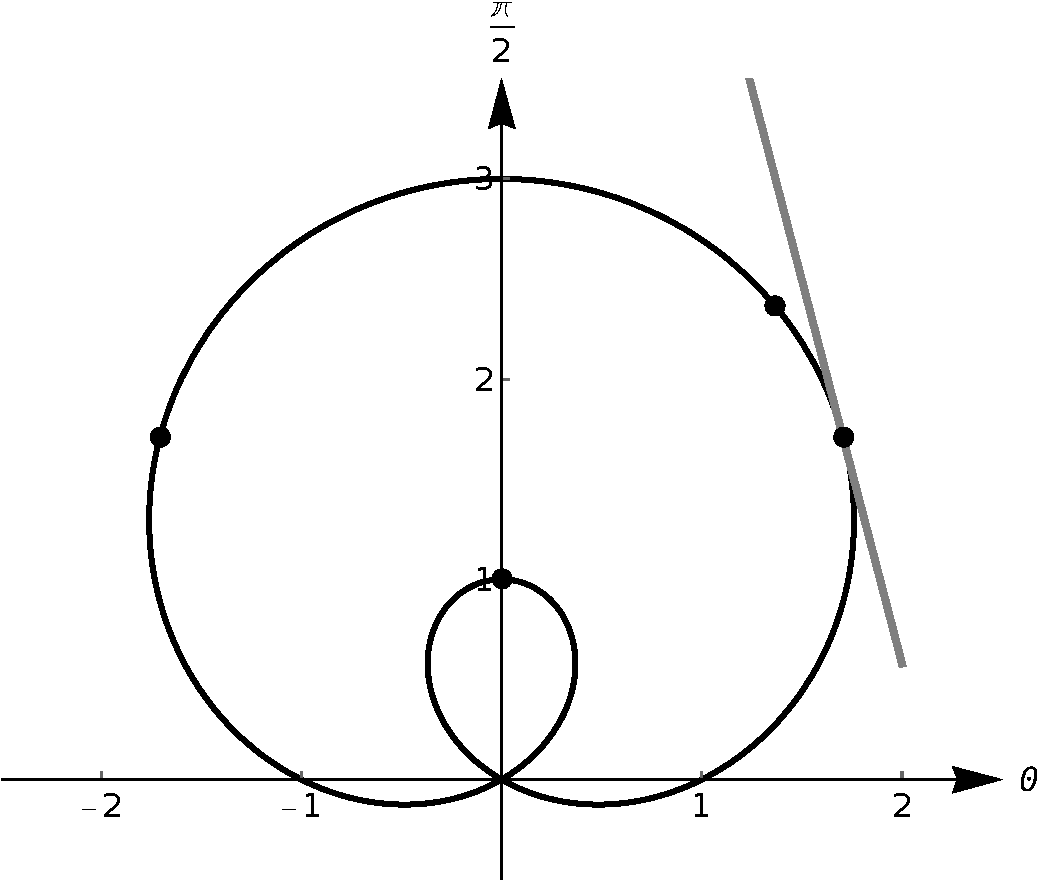
\includegraphics[width=0.5\textwidth]{fig_parametric_20}
	\caption{The lima\c con in Example \ref{ex_polcalc1} with its tangent line at $\theta=\pi/4$ and points of vertical and horizontal tangency.}
	\label{fig_parametric_20}
	\end{center}
\end{figure}


\end{example}


\subsection{Smoothness}
For what concerns the smoothness of parametric curves, we have the following -- stricter -- definition in order to arrive at curves without corners. 

\begin{definition}[Smoothness of a parametric curve]\label{def:smooth2}
A curve $C$ defined by $x=f(t)$, $y=g(t)$ is \textbf{smooth} (\textit{glad}) on an interval $I$ if $\fp$ and $g'$ are continuous on $I$ and not simultaneously 0 (except possibly at the endpoints of $I$). A curve is \textbf{piecewise smooth} (\textit{stuksgewijs glad}) on $I$ if $I$ can be partitioned into subintervals where $C$ is smooth on each subinterval.
\end{definition}
\index{smooth!function}\index{cusp}\index[aut]{functie ! glad}\index{function ! smooth}\index{smoothness}

The continuity condition is in agreement with Definition~\ref{def:smooth} and relates to parameterizations that could fail to be differentiable at a point. The second condition, however, relates to parameterizations that could slow to a stop, and then start up again in a completely different direction.  Indeed, if a curve is not smooth at $t=t_0$, it means that $x'(t_0)=y'(t_0)=0$ as defined. This, in turn, means that rate of change of $x$ (and $y$) is 0; that is, at that instant, neither $x$ nor $y$ is changing. If the parametric equations describe the path of some object, this means the object is at rest at $t_0$. An object at rest can make a sharp change in direction, whereas moving objects tend to change direction in a smooth fashion.


Consider the astroid, given by $x=\cos^3(t)$, $y=\sin^3(t)$ (Figure~\ref{fig_parametric_18}). Taking derivatives, we have:
$$x' = -3\cos^2(t)\sin (t)\quad \text{and}\quad y' = 3\sin^2(t)\cos (t).$$
It is clear that each is 0 when $t=0,\ \pi/2,\ \pi,\ldots\,.$ Thus the astroid is not smooth at these points, corresponding to the cusps seen in Figure~\ref{fig_parametric_18}.

\begin{example}\label{ex_pareq9}
Let a curve $C$ be defined by the parametric equations $x=t^3-12t+17$ and $y=t^2-4t+8$. Determine the points, if any, where it is not smooth.

\xhrulefill{gray}{2.5pt}Solution \xhrulefill{gray}{2.5pt}

We begin by taking derivatives. 
$$x' = 3t^2-12,\text{ and } y' = 2t-4.$$
We set each equal to 0. It follows that 
$$
x' = 0 \quad\Leftrightarrow\quad 3t^2-12=0 \quad\Leftrightarrow\quad t=\pm 2,
$$
and
$$
  y'=0 \quad\Leftrightarrow\quad 2t-4 = 0 \quad\Leftrightarrow\quad t=2.
	$$
We see that at $t=2$ both $x'$ and $y'$ are 0; thus $C$ is not smooth at $t=2$, corresponding to the point $(1,4)$. The curve is graphed in Figure \ref{fig_parametric_21}, illustrating the cusp at $(1,4)$.


\begin{figure}[H]
	\begin{center}
			\includegraphics[width=0.5\textwidth]{fig_parametric_21}
	\caption{Graphing the curve in Example \ref{ex_pareq9}; note it is not smooth at $(1,4)$.}
	\label{fig_parametric_21}
	\end{center}
\end{figure}


\end{example}

One should be careful to note that a sharp corner does not have to occur when a curve is not smooth. For instance, one can verify that $x=t^3$ and $y=t^6$ produce the familiar $y=x^2$ parabola. However, in this parametrization, the curve is not smooth. A particle travelling along the parabola according to the given parametric equations comes to rest at $t=0$, though no sharp point is created.

\subsection{Concavity}
 \ifcourse
 	\checkoddpage
\marginpar{\ifoddpage\hspace*{-1.5cm}\else\hspace*{0.25cm}\fi\includegraphics[width=0.075\textwidth]{youtube}\\
\ifoddpage\hspace*{-1.75cm}\else\hspace*{0.1cm}\fi
\qrcode[height=1.75cm]{https://youtu.be/AXasQLqazWU}
%\includegraphics[width=0.1\textwidth]{diff2_para_vgln}
}
 \fi
For what concerns curves in the plane described by means of parametric equations, we may also  consider their concavity; that is, we are interested in $\frac{d^2y}{dx^2}$. To find this, we need to find the derivative of $\frac{dy}{dx}$ with respect to $x$; that is,  $$\frac{d^2y}{dx^2}=\frac{d}{dx}\left[\frac{dy}{dx}\right],$$ but recall that $\frac{dy}{dx}$ is a function of $t$, not $x$, making this computation not straightforward. \index{concavity}\index[aut]{concaviteit}

Let now $h(t) = \frac{dy}{dx}$. We want $\frac{d}{dx}[h(t)]$, which follows from the chain rule. Indeed, we have
$$\frac{dh}{dt} = \frac{dh}{dx}\cdot\frac{dx}{dt} \quad \Rightarrow \quad \frac{dh}{dx} = \frac{\quad\dfrac{dh}{dt}\quad}{\dfrac{dx}{dt}}\,.$$

Hence, this leads to
\begin{equation}
\frac{d^2y}{dx^2}\quad = \quad\frac{\quad\dfrac{d}{dt}\left[\dfrac{dy}{dx}\right]\quad}{\dfrac{dx}{dt}} \quad=\quad\frac{\quad\dfrac{d}{dt}\left[\dfrac{dy}{dx}\right]\quad}{\fp(t)}\,.
\label{idea:second_der_par}
\end{equation}


An example will help us understand this.

\begin{example}\label{ex_parcalc4}
Let $x=5t^2-6t+4$ and $y=t^2+6t-1$ as in Example \ref{ex_parcalc1}. Determine the $t$-intervals on which the graph is concave up/down.

\xhrulefill{gray}{2.5pt}Solution \xhrulefill{gray}{2.5pt}

Concavity is determined by the second derivative of $y$ with respect to $x$, $\frac{d^2y}{dx^2}$, so we compute that here following Equation~\eqref{idea:second_der_par}.

In Example \ref{ex_parcalc1}, we found $\frac{dy}{dx} = \frac{2t+6}{10t-6}$ and $\fp(t) = 10t-6$. So:
\begin{align*}
\frac{d^2y}{dx^2} &=\frac{\quad\dfrac{d}{dt}\left[\dfrac{2t+6}{10t-6}\right]\quad}{10t-6}  \\[0.2cm]
				&= -\frac{\quad\dfrac{72}{(10t-6)^2}\quad}{10t-6}\\[0.2cm]
				&= -\frac{72}{(10t-6)^3} \\[0.2cm] &= -\frac{9}{(5t-3)^3}.
\end{align*}

The graph of the parametric functions is concave up when $\frac{d^2y}{dx^2} > 0$ and concave down when $\frac{d^2y}{dx^2} <0$. We determine the intervals when the second derivative is greater/less than 0 by first finding when it is 0 or undefined.

As the numerator of $ -\frac{9}{(5t-3)^3}$ is never 0, $\frac{d^2y}{dx^2} \neq 0$ for all $t$. It is undefined when $5t-3=0$; that is, when $t= 3/5$. Following the work established in Section~\ref{sec:concavity}, we look at values of $t$ greater/less than $3/5$ on a number line:

\begin{center}\begin{tikzpicture}[>=latex]
		\draw [<->, thick] (-2.5,0) -- (2.5,0);
		\foreach \x / \y  in %
					{0/{$3/5$}}
		{\draw (\x,-.3) node[below] {\scriptsize \parbox{40pt}{\centering \y}} -- (\x,.3);}
		\draw (-1,.75) node {\scriptsize \parbox{50pt}{\centering $\ds \frac{d^2y}{dx^2}>0$ \\[5pt] c. up }};
		\draw (1,.75) node {\scriptsize \parbox{50pt}{\centering $\ds\frac{d^2y}{dx^2}<0$ \\[5pt] c. down }};
\end{tikzpicture}\end{center}

Reviewing Example \ref{ex_parcalc1}, we see that when $t=3/5=0.6$, the graph of the parametric equations has a vertical tangent line. This point is also a point of inflection for the graph, illustrated in Figure \ref{fig_parametric_22}.

		\begin{figure}[H]
	\begin{center}
			\includegraphics[width=0.4\textwidth]{fig_parametric_22}
	\caption{Graphing the parametric equations in Example \ref{ex_parcalc4} to demonstrate concavity.}
	\label{fig_parametric_22}
	\end{center}
\end{figure}


\end{example}




\newpage
\section{Exercises}

\renewcommand{\ExerciseListName}{Assignement}

\subsection*{\nameref{sec_polar}}
%%%%%%%%%%%%%%%%%%
%Oefening 1
%%%%%%%%%%%%%%%%%%	
\begin{Exercise}[difficulty = 1] Which of the following pairs of polar coordinates represents the same point? 
		%\begin{multicols}{3}
			\Question $(3,0) = (-3,\pi)$
			\Question $(-3,0) = (-3,2\pi)$
			\Question $\left(2, \dfrac{2 \pi}{3} \right) = \left(-2, -\dfrac{\pi}{3} \right)$
			\Question $\left(2, \dfrac{7 \pi}{3} \right)=\left(2, \dfrac{\pi}{3} \right)=\left(2, \dfrac{13\pi}{3} \right)$
			\EndCurrentQuestion
		%\end{multicols}

\end{Exercise}

\setboolean{firstanswerofthechapter}{true}
\begin{Answer}\phantom{}
		\begin{multicols}{2}
			\Question $(3,0)$
			\Question $(-3,0)$
			\Question $\left(2, \dfrac{2 \pi}{3} \right)$
			\Question  $\left(2, \dfrac{7 \pi}{3} \right)$
			\Question  $(-3, \pi)$
			\Question  $\left(2, \dfrac{\pi}{3}\right)$
			\Question  $(-3, 2\pi)$ 
			\Question  $\left(-2, -\dfrac{\pi}{3} 			\right)$
			\Question  $\left(2, \dfrac{13\pi}{3} \right)$
			\EndCurrentQuestion
		\end{multicols}
\end{Answer}
\setboolean{firstanswerofthechapter}{false}

%%%%%%%%%%%%%%%%%%%%%
%Oefening 2
%%%%%%%%%%%%%%%%%%%%%	
\begin{Exercise}[difficulty = 1] Determine the Cartesian coordinates for the following points given in polar coordinates. 
		\begin{multicols}{3}
			\Question $\left( \sqrt{2}, \dfrac{\pi}{4} \right)$
			\Question $\left(1,0 \right)$
			\Question $(0, \pi)$
			\Question $\left( -\sqrt{2}, \dfrac{\pi}{4} \right)$
		%	\Question $\left(5, \arctan \dfrac{4}{3} \right)$
			\Question $\left(2 \sqrt{3}, \dfrac{2\pi}{3} \right)$
			\EndCurrentQuestion
		\end{multicols}

\end{Exercise}

\begin{Answer}\phantom{}
    
		\begin{multicols}{3}
			\Question $\left( 1,1\right)$
			\Question $\left(1,0 \right)$
			\Question $(0, 0)$
			\Question $\left( -1, -1 \right)$
			\Question $\left(- \sqrt{3}, 3 \right)$
			\EndCurrentQuestion
		\end{multicols}
\end{Answer}

%%%%%%%%%%%%%%%%%%%%%
%Oefening 3
%%%%%%%%%%%%%%%%%%%%%
\begin{Exercise} Convert the given polar equation into a Cartesian equation and name the curve. 
		\begin{multicols}{2}
			\Question[difficulty = 1] $\theta = \dfrac{\pi}{4}$
			\Question[difficulty = 1] $r = \dfrac{7}{5 \sin (\theta) - 2\cos (\theta)}$ 
			\Question[difficulty = 1] $r=2\cos(\theta)$ 
			\Question[difficulty = 1] $r = -4 \sin(\theta)$ 				
			\Question[difficulty = 1] $r = \sin (\theta) + \cos (\theta)$
			\ifanalysis\Question[difficulty = 1]\fi\ifcalculus\Question[difficulty = 2]\fi $r = \dfrac{2}{\sqrt{\cos^2 (\theta) + 4 \sin^2 (\theta)}}$
			\Question[difficulty = 2] $r = \dfrac{1}{1- \cos (\theta)}$
			\Question[difficulty = 2] $r = \dfrac{1}{1- 2\sin (\theta)}$
	        \EndCurrentQuestion
		\end{multicols}

\end{Exercise}

\begin{Answer}\phantom{}
    
	\begin{multicols}{2}
	  \Question $y=x$ \qquad $\rightarrow $ line
    	\Question $y = \dfrac{2}{5} x +  \dfrac{7}{5}$ \qquad $\rightarrow $ line  
    	\Question $(x-1)^2+ y^2=1$ \qquad $\rightarrow $ circle
    	\Question $x^2 + (y+2)^2 = 4$ \qquad $\rightarrow $ circle 
		\Question $\left(x-\dfrac{1}{2}\right)^2 + \left(y-\dfrac{1}{2}\right)^2= \dfrac{1}{2}$\qquad $\rightarrow $ circle
		\Question $x^2+4y^2=4$\qquad $\rightarrow $ ellipse
		\Question $y^2 = 1+2x$\qquad $\rightarrow $ parabola
		\Question $-3 x^2 + 9 \left( y + \dfrac{2}{3} \right)^2 = 1$\qquad $\rightarrow $ hyperbola
		\EndCurrentQuestion
	\end{multicols}
\end{Answer}
	
	
\ifanalysis \pagebreak \fi		
%%%%%%%%%%%%%%%%%%%%%
%Oefening 4
%%%%%%%%%%%%%%%%%%%%%
\begin{Exercise}[label = oef_poolkrommes_tekenen] Sketch the graph of the curves below.
    \begin{multicols}{2}
	    \Question[difficulty = 1] $r=2\qquad \left( 0 \leq \theta \leq \dfrac{\pi}{2} \right)$
	    \Question[difficulty = 1] $r = 2 - \sin (\theta)$
		\Question[difficulty = 1] $r = \dfrac{3}{2 \cos (\theta) - \sin (\theta)} $ 
		\Question[difficulty = 1] $r = 2 + 4 \cos(\theta)$ 
		\Question[difficulty = 1] $r = 5\sin(2\theta)$ 
		\Question[difficulty = 1] $r = 2\sin (2\theta)$ 
		\Question[difficulty = 1] $r=\cos \left( \dfrac{2\theta}{3} \right) \qquad \left( 0 \leq \theta \leq 6\pi \right)$ 
		\Question[difficulty = 1] $r=3\sin \left( \theta\right) \qquad \left( 0 \leq \theta \leq \pi \right)$
		\Question[difficulty = 1] $r=3\csc \left( \theta\right) \qquad \left( 0 <\theta < \pi \right)$
		\Question[difficulty = 2] $r^2 = 4 \sin (2\theta)$ 
		\Question[difficulty = 2] $r^2 = 4 \cos (3\theta)$  
		\Question[difficulty = 2] $r^2 = \sin (3\theta)$ 
		\ifanalysis
		\Question[difficulty = 2] $r = a \sqrt{\cos (2 \theta)}\qquad (a > 0)$
		\Question[difficulty = 2] $r = a \cos (n \theta) \qquad (a > 0, n \in \mathbb{Z})$
		\Question[difficulty = 2] $r = \dfrac{a}{\theta}\qquad (a > 0)$
		\fi
	    \EndCurrentQuestion
	\end{multicols}

\end{Exercise}

\begin{Answer}\phantom{}
    Consider the graphs below.% Figuur \ref{fig_poolkrommes} en \ref{fig_poolkrommes_deel2}.  
    
      \begin{figure}[H]
            \centering
            \centerline{
            \subfigure[$r=2, 0 \leq \theta \leq  \dfrac{\pi}{2}$ \label{fig_oef_poolkromme_a} ]{\includegraphics[width=0.3\textwidth]{fig_parametric_oef_4a}} 
            \hspace{0.1cm}
            \subfigure[$r = 2 - \sin (\theta)$\label{fig_oef_poolkromme_b}]{\includegraphics[width=0.3\textwidth]{fig_parametric_oef_4b}} %}  
            \hspace{0.1cm}
            \subfigure[$r = \dfrac{3}{2 \cos (\theta) - \sin (\theta)}$\label{fig_oef_poolkromme_c}]{\includegraphics[width=0.3\textwidth]{fig_parametric_oef_4c}}  
            }
            \centerline{
            \subfigure[$r=2+4\cos(\theta)$\label{fig_oef_poolkromme_d}]{\includegraphics[width=0.3\textwidth]{fig_parametric_oef_4d}} 
            \hspace{0.1cm}
            \subfigure[$r = 5\sin(2\theta)$\label{fig_oef_poolkromme_e}]{\includegraphics[width=0.3\textwidth]{fig_parametric_oef_4e}} 
            \hspace{0.1cm}
            \subfigure[$r = 2\sin (2\theta)$ \label{fig_oef_poolkromme_f}]{\includegraphics[width=0.3\textwidth]{fig_parametric_oef_4f}}  
            }
             \centerline{
             \subfigure[$r = \cos (2\theta/3), 0 \leq \theta \leq 6\pi$ \label{fig_oef_poolkromme_g}]{\includegraphics[width=0.3\textwidth]{fig_parametric_oef_4g}} 
            \hspace{0.1cm}
            \subfigure[$r = 3 \sin(\theta), 0 \leq \theta \leq \pi $\label{fig_oef_poolkromme_h}]{\includegraphics[width=0.3\textwidth]{fig_parametric_oef_4h}} 
            \hspace{0.1cm}
            \subfigure[$r = 3\csc (\theta), 0 < \theta < \pi$ \label{fig_oef_poolkromme_i}]{\includegraphics[width=0.3\textwidth]{fig_parametric_oef_4i}} % 
            }
            \caption{Graphs of the polar curves in Ex.~\ref{oef_poolkrommes_tekenen} (deel 1).}
            \label{fig_poolkrommes}
            \end{figure}
            
		    \begin{figure}[H]
            \centering
            \centerline{
            \addtocounter{subfigure}{9}
            \subfigure[$r^2 = 4 \sin (2\theta)$ \label{fig_oef_poolkromme_j}]{\includegraphics[width=0.3\textwidth]{fig_parametric_oef_4j}} 
            \hspace{0.1cm}
            \subfigure[$r^2 = 4 \cos(3\theta)$\label{fig_oef_poolkromme_k}]{\includegraphics[width=0.3\textwidth]{fig_parametric_oef_4k}} 
            \hspace{0.1cm}
            \subfigure[$r^2 = \sin (3\theta)$ \label{fig_oef_poolkromme_l}]{\includegraphics[width=0.3\textwidth]{fig_parametric_oef_4l}} % 
            }
            \centerline{
            \subfigure[$r = a \sqrt{\cos (2 \theta)}, \quad a > 0$. Links $a=1$, \quad  right $a=2$\label{fig_oef_poolkromme_m} ]{\includegraphics[width=0.3\textwidth]{fig_parametric_oef_4ma} \qquad
		    \includegraphics[width=0.3\textwidth]{fig_parametric_oef_4mb}} 
            }
            \centerline{
            \subfigure[$r = a \cos (n \theta), \quad a > 0$. If $n$ is odd, the curve has $n$ 'leaves'. If $n$ is even, the curve has $2n$ 'leaves'. The curve was plotted for $n=3$ (left) and $n=4$ (right).\label{fig_oef_poolkromme_k} ]{\includegraphics[width=0.3\textwidth]{fig_parametric_oef_4na} \qquad
		    \includegraphics[width=0.3\textwidth]{fig_parametric_oef_4nb}} 
            }
            \centerline{
            \subfigure[$r = a/\theta$. The curve was plotted for $a=2$ with two different intervals for $\theta$. Left: $0 \leq \theta \leq 2\pi$, \quad right: $0 \leq \theta \leq 4\pi$.  \label{fig_oef_poolkromme_l} ]{\includegraphics[width=0.3\textwidth]{fig_parametric_oef_4oa} \qquad
		    \includegraphics[width=0.3\textwidth]{fig_parametric_oef_4ob}} 
            }
            \caption{Graphs of the polar curves in Exercise~\ref{oef_poolkrommes_tekenen} (part 2).}
            \label{fig_poolkrommes_deel2}
        \end{figure}
\end{Answer}

%%%%%%%%%%%%%%%%%%%%%
%Oefening 5
%%%%%%%%%%%%%%%%%%%%%
\begin{Exercise} Determine the intersection(s) of the graphs represented by the polar equations below.
\begin{multicols}{2}
	\Question[difficulty = 1] $r = 3 \cos (\theta), \quad r = 1 + \cos (\theta)$ 
	\ifanalysis\Question[difficulty = 1]\fi\ifcalculus\Question[difficulty = 2]\fi $r = \sec^2 \left(\dfrac{\theta}{2} \right), \quad r = 3\csc^2 \left(\dfrac{\theta}{2} \right)$ 
	\Question[difficulty = 1] $r=\sin (\theta), \quad r = 1 - \sin (\theta)$ 
	\Question[difficulty = 1] $r= \sqrt{3} \cos (\theta), \quad r = \sin (\theta)$
	\Question[difficulty = 1] $r^2=2 \cos (2\theta), \quad r = 1$
	\Question[difficulty = 1] $r= \sin (3\theta), \quad r = \cos (3\theta), \quad [0, \pi]$
	\Question[difficulty = 1] $r= 1-\cos (\theta), \quad r = 1+\sin (\theta), \  [0, 2\pi]$ 
    \EndCurrentQuestion
\end{multicols}

\end{Exercise}

\begin{Answer}\phantom{}
    
			\Question The origin \, and \, $\left(\dfrac{3}{2}, \pm \dfrac{\pi}{3}\right)$
			\Question $\left(4, \pm \dfrac{2\pi}{3}\right)$
			\Question The origin, \, $\left(\dfrac{1}{2}, \dfrac{\pi}{6}\right)$ \, and \, $\left(\dfrac{1}{2}, \dfrac{5\pi}{6}\right)$
			\Question The origin \, and \, $\left(\dfrac{\sqrt{3}}{2}, \dfrac{\pi}{3}\right)$  
			\Question $\left(1, \pm \dfrac{\pi}{6}\right)$ \, and \, $\left(1, \pm \dfrac{5\pi}{6}\right)$  
            \Question The origin, \, $\left(\dfrac{\sqrt{2}}{2}, \dfrac{\pi}{12}\right)$\, and \, $\left(-\dfrac{\sqrt{2}}{2}, \dfrac{5\pi}{12}\right)$  
            \Question The origin, \, $\left(1+\dfrac{\sqrt{2}}{2}, \dfrac{3\pi}{4}\right)$\, and \,$\left(1-\dfrac{\sqrt{2}}{2}, \dfrac{7\pi}{4}\right)$
		
\end{Answer}

\subsection*{\nameref{sec:parameter_eq}}

%%%%%%%%%%%%%%%%%%%%%
%Oefening 6
%%%%%%%%%%%%%%%%%%%%%	
\begin{Exercise}[label=oef_parameterkrommes_tekenen] Determine the Cartesian equation of the given parameter representation  and draw the corresponding curve. 
	\begin{multicols}{2}
		\Question[difficulty = 1] $\left\{\begin{array}{l} x = 2-t \\[0.5cm] y = t+1 \end{array}\right.\qquad (0 < t < + \infty) $ 
		\Question[difficulty = 1] $\left\{\begin{array}{l} x = \dfrac{1}{t} \\[0.5cm] y = t-1 \end{array}\right.\qquad (0 < t < 4) $	
		\Question[difficulty = 2] $\left\{\begin{array}{l} x = \dfrac{1}{1+t^2} \\[0.5cm] y = \dfrac{t}{1+t^2} \end{array}\right.\qquad (t \in \mathbb{R})$
		\ifanalysis\Question[difficulty = 1]\fi\ifcalculus\Question[difficulty = 2]\fi $\left\{\begin{array}{l} x = 3 \sin (2t) \\ y = 3 \cos (2t) \end{array}\right.\qquad \left(0 \leq t \leq \dfrac{\pi}{3} \right) $ 
		\Question[difficulty = 2] $\left\{\begin{array}{l} x = 1-\sqrt{4-t^2} \\ y = 2+t \end{array}\right.\qquad (-2 \leq t \leq 2) $  
		\Question[difficulty = 2] $\left\{\begin{array}{l} x = \sec(t) \\ y = \tan(t) \end{array}\right.\qquad (t \in \mathbb{R}) $
		\Question[difficulty = 1] $\left\{\begin{array}{l} x = e^t \\ y = e^{3t} - 3 \end{array}\right.\qquad (t \in \mathbb{R})$ 
		\ifanalysis
		\Question[difficulty = 2] $\left\{\begin{array}{l} x = \cos (\sin (s)) \\ y = \sin (\sin (s)) \end{array}\right.\qquad (s \in \mathbb{R})$	
		\Question[difficulty = 1] $\left\{\begin{array}{l} x = \cosh(t) \\ y = \sinh(t) \end{array}\right.\qquad (t \in \mathbb{R}) $ 
		\fi
		\EndCurrentQuestion
	\end{multicols}
	
\end{Exercise}

\begin{Answer}\phantom{}
    Consider the graphs below. % Figuur~\ref{fig_parameterkrommes}. 
    
    	   \begin{figure}[H]
            \centering
            \centerline{
            \subfigure[$y=3-x \qquad (-\infty< x < 2 )$\label{fig_oef_parameterkromme_a}]{\includegraphics[width=0.3\textwidth]{fig_parametric_oef_6a}}  
            \hspace{0.1cm}
            \subfigure[$y= \dfrac{1}{x} - 1 \qquad \left( x > \dfrac{1}{4} \right)$\label{fig_oef_parameterkromme_b}]{\includegraphics[width=0.3\textwidth]{fig_parametric_oef_6b}} 
            \hspace{0.1cm}
            \subfigure[$\left(x-\dfrac{1}{2}\right)^2 + y^2= \dfrac{1}{4}$\label{fig_oef_parameterkromme_c}]{\includegraphics[width=0.3\textwidth]{fig_parametric_oef_6c}} 
            }
            \centerline{
            \subfigure[$x^2 + y^2 = 9$ \quad (part of the circle indicated on the figure) \label{fig_oef_parameterkromme_d}]{\includegraphics[width=0.3\textwidth]{fig_parametric_oef_6d}}  
            \hspace{0.5cm}
            \subfigure[$(x-1)^2 + (y-2)^2= 4 \qquad (x\leq 1) $ \label{fig_oef_parameterkromme_e}]{\includegraphics[width=0.3\textwidth]{fig_parametric_oef_6e}} 
            \hspace{0.5cm}
            \subfigure[$x^2 - y^2= 1$ \label{fig_oef_parameterkromme_f}]{\includegraphics[width=0.3\textwidth]{fig_parametric_oef_6f}} 
            }
            \centerline{
            \subfigure[$y=x^3-3$ \label{fig_oef_parameterkromme_g}]{\includegraphics[width=0.3\textwidth]{fig_parametric_oef_6g}}  
            \hspace{0.5cm}
            \ifanalysis
            \hspace{0.5cm}
            \subfigure[$x^2 + y^2 = 1$. 
            \label{fig_oef_parameterkromme_h}]{\includegraphics[width=0.3\textwidth]{fig_parametric_oef_6h}} 
            \hspace{0.5cm}
            \subfigure[$x^2-y^2=1  \qquad (x \geq 1) $ \label{fig_oef_parameterkromme_i}]{\includegraphics[width=0.2\textwidth]{fig_parametric_oef_6i}} 
            \fi
            }
            \caption{Graphs of the parametric curves in Exercise~\ref{oef_parameterkrommes_tekenen}.}
            \label{fig_parameterkrommes}
        \end{figure}
\end{Answer}
	
%%%%%%%%%%%%%%%%%%%%%
%Oefening 7
%%%%%%%%%%%%%%%%%%%%%
\begin{Exercise} Determine a parametrization of the curves below. 
	\Question[difficulty = 1] The lower half of the parabola $y^2 = x-1$.
	\Question[difficulty = 2] $x^{2/3} + y^{2/3} = 6^{2/3}$

\end{Exercise}

\begin{Answer}\phantom{}
    \begin{multicols}{2}
	
		\Question $\left\{\begin{array}{l} x = t \\[0.5cm] y = - \sqrt{t-1} \end{array}\right.\qquad (t>1) $
		\Question $\left\{\begin{array}{l} x = 6 \cos^3(t) \\[0.5cm] y =  6 \sin^3(t) \end{array}\right.\qquad (0<t<2 \pi) $
\EndCurrentQuestion
	\end{multicols}
\end{Answer}

%%%%%%%%%%%%%%%%%%%%%
%Oefening 8
%%%%%%%%%%%%%%%%%%%%%
\begin{Exercise}[difficulty = 1] Use $t=y$ to paramterize the intersection of the planes $y=2x-4$ and $z=3x+1$ between $(2,0,7)$ and $(3,2,10)$. 

\end{Exercise}

\begin{Answer}\phantom{}
    $\vec r (t) = \left( \dfrac{t+4}{2}, t , \left(\dfrac{3}{2}t+7 \right) \right)$\quad with $\ 0 \leq t \leq 2 $
\end{Answer}

%%%%%%%%%%%%%%%%%%%%%
%Oefening 9
%%%%%%%%%%%%%%%%%%%%%
\begin{Exercise}[difficulty = 1] The curve of intersection of the plane $x+y=1$ with the paraboloid $z = x^2 + y^2$ is a parabola. Parameterize this  parabola  using $t=x$ as a parameter. Can you use $t=y$ as well? What about $t=z$?  %vb 2 pg. 637 

\end{Exercise}

\begin{Answer}\phantom{}\\
    parameter $t=x$: \quad $\vec r (t) = \left( t, 1-t, 1-2t+2t^2 \right) $\quad with $\  - \infty < t < + \infty$\\
    parameter $t=y$: \quad $\vec r (t) = \left(1-t, t, 1-2t+2t^2 \right) $\quad with $\ - \infty < t < + \infty$\\
    parameter $t=z$: We have to solve the system of equations  $\left\{\begin{array}{l} x+y=1 \\ x^2+y^2=t \end{array}  \right.$ for $x$ and $y$. There are two possible solutions each corresponding to one half of the parabola starting at the lowest point $(1/2,1/2,1/2) $ because there are two points on the parabola at every  $z>1/2$. The entire parabola can not be parameterized by using $z$ as a parameter.
\end{Answer}
    
%%%%%%%%%%%%%%%%%%%%%
%Oefening 10
%%%%%%%%%%%%%%%%%%%%% 
\begin{Exercise} Parameterize the curve that defines  the intersection between the given curves. %oef 7,8,9 par 11.3 pg 643
     \begin{multicols}{2}
         \Question[difficulty = 1] $x^2+y^2 = 9$ \quad and \quad $z=x+y$
         \Question[difficulty = 1] $z=\sqrt{1-x^2-y^2}$ \quad and \quad $x+y=1$
         \Question[difficulty = 2] $z = x^2+y^2$\quad and \quad $2x-4y-z-1=0$
        \EndCurrentQuestion
	 \end{multicols}
	
\end{Exercise}

\begin{Answer}\phantom{}
    
         \Question $x^2+y^2 = 9$ \quad and \quad $z=x+y$ 
         
          A possible parameterization is $\ \vec r(t) = (3 \cos (t), 3 \sin (t), 3(\cos(t) + \sin(t)))$.
         \Question $z=\sqrt{1-x^2-y^2}$ \quad and \quad $x+y=1$ 
         
          A possible parameterization is $\ \vec r(t) = \left(t, 1-t, \sqrt{2(t-t^2)}\right)$.
         \Question $z = x^2+y^2$\quad and \quad $2x-4y-z-1=0$ 
         
          A possible parameterization is $\ \vec r(t) = (1+2\cos(t),-2(1- \sin(t)), 9+4 \cos(t)-8\sin(t))$.
     
\end{Answer}

\ifcalculus\pagebreak\fi
%%%%%%%%%%%%%%%%%%%%%
%Oefening 11
%%%%%%%%%%%%%%%%%%%%%	
\begin{Exercise}[label = oef_parameterkrommes_tekenen2] Sketch the graph of the curves given by the parameter representations below. 
	\begin{multicols}{2}
		\Question[difficulty = 1] $\left\{\begin{array}{l} x = t^2 \\ y = 2 \end{array}\right. \qquad (-2  \leq t \leq 2) $
		\Question[difficulty = 1] $\left\{\begin{array}{l} x = t-1 \\ y = 2t+3 \end{array}\right. \qquad (- \infty < t < + \infty) $
		\Question[difficulty = 1] $\left\{\begin{array}{l} x = t^2 \\ y = t-3 \end{array}\right. \qquad (- \infty < t < + \infty) $
		\ifanalysis\Question[difficulty = 1]\fi\ifcalculus\Question[difficulty = 2]\fi $\left\{\begin{array}{l} x = \sin (t) \\ y = \cos^2 (t) \end{array}\right. \qquad \left(0 \leq t \leq \dfrac{3\pi}{2} \right) $
		\Question[difficulty = 2] $\left\{\begin{array}{l} x = -2\sin (t) \\ y = 3\cos (t) \end{array}\right. \qquad \left(0 \leq t \leq 3\pi \right) $
		\Question[difficulty = 1] $\left\{\begin{array}{l} x = 2t \\ y = t^3+4 \end{array}\right. \qquad (-2  \leq t \leq 2) $
	    \EndCurrentQuestion
	\end{multicols}

\end{Exercise}

\begin{Answer}\phantom{}
    Consider the graphs below.% Figuur~\ref{fig_parameterkrommes2}.
    \begin{figure}[H]
            \centering
            \centerline{
            \subfigure[\label{fig_oef_parameterkromme_11a}]{\includegraphics[width=0.3\textwidth]{fig_parametric_oef_11a}}
            \hspace{0.5cm}
            \subfigure[\label{fig_oef_parameterkromme_11b}]{\includegraphics[width=0.3\textwidth]{fig_parametric_oef_11b}}
            \hspace{0.5cm}
            \subfigure[\label{fig_oef_parameterkromme_11c}]{\includegraphics[width=0.3\textwidth]{fig_parametric_oef_11c}}
            }
            \centerline{
            \hspace{0.7cm}
            \subfigure[\label{fig_oef_parameterkromme_11d}]{\includegraphics[width=0.3\textwidth]{fig_parametric_oef_11d}}
            \hspace{0.7cm}
            \subfigure[\label{fig_oef_parameterkromme_11e}]{\includegraphics[width=0.2\textwidth]{fig_parametric_oef_11e}}
            \hspace{0.7cm}
            \subfigure[\label{fig_oef_parameterkromme_11f}]{\includegraphics[width=0.2\textwidth]{fig_parametric_oef_11f}}
            }
            \caption{Grafieken van de parameterkrommen in Oefening~\ref{oef_parameterkrommes_tekenen2}.}
            \label{fig_parameterkrommes2}
        \end{figure}
\end{Answer}

%%%%%%%%%%%%%%%%%%%%%
%Oefening 12 Bio-irs
%%%%%%%%%%%%%%%%%%%%%
\ifanalysis
\begin{Exercise}[difficulty = 2] Describe the similarities and differences between the graphs belonging to the parametric equations below.  %Apex: oef 9.2.19
    \Question $x = \cos(t), \quad y=\sin(t) \qquad \left(0 \leq t \leq 2\pi \right)$
    \Question $x = \cos \left(t^2\right), \quad y=\sin \left(t^2\right) \qquad \left(0 \leq t \leq 2\pi \right)$
    \Question $x = \cos \left(1/t\right), \quad y=\sin \left(1/t\right) \qquad \left(0 < t <1 \right)$
    \Question $x = \cos \left(\cos(t) \right), \quad y=\sin \left(\cos(t) \right) \qquad \left(0 \leq t \leq 2\pi \right)$

\end{Exercise}

\begin{Answer}\phantom{}
     
        \Question Circle with radius 1, counterclockwise, 1 loop.  
        \Question Circle with radius 1, counterclockwise, 6 loops.  
        \Question Circle of radius 1, clockwise,  infinite number of loops. 
        \Question Arc of a circle of radius 1, from angle $-1$ radians to $1$ radians, 2 loops. 
    
\end{Answer}
\fi

%%%%%%%%%%%%%%%%%%%%%
%Oefening 13 Bio-irs
%Oefening 12 Ings
%%%%%%%%%%%%%%%%%%%%%

\begin{Exercise}[difficulty = 2, label = oef_match_graphs_par_eq_curves_opl] Determine which graphs of $x=f(t)$ and $y=f(t)$ in Figure~\ref{fig_parametric_23} belong to the graphs of the parametric curves in Figure~\ref{fig_parametric_24}. \label{oef_match_graphs_par_eq_curves}
    \begin{figure}[H]
    \centerline{
    \subfigure[\label{fig_parametric_23a}]{\includegraphics[width=0.4\textwidth]{fig_parametric_23a}}
    \hspace{1cm}
    \subfigure[\label{fig_parametric_23b}]{\includegraphics[width=0.4\textwidth]{fig_parametric_23b} }
    }
    \centerline{
    \subfigure[\label{fig_parametric_23c}]{\includegraphics[width=0.4\textwidth]{fig_parametric_23c} }
    \hspace{1cm}
    \subfigure[\label{fig_parametric_23d}]{\includegraphics[width=0.4\textwidth]{fig_parametric_23d} }
    }
    \caption{Graphs of the parametric equations from Exercise~\ifanalysis 13\fi \ifcalculus 12\fi. }
    \label{fig_parametric_23}
    \end{figure}
    
    \begin{figure}[H]
    \centerline{
    \subfigure[\label{fig_parametric_24a}]{\includegraphics[width=0.2\textwidth]{fig_parametric_24a}}
    \hspace{1cm}
    \subfigure[\label{fig_parametric_24b}]{\includegraphics[width=0.2\textwidth]{fig_parametric_24b} }
    }
    \centerline{
    \subfigure[\label{fig_parametric_24c}]{\includegraphics[width=0.2\textwidth]{fig_parametric_24c} }
    \hspace{1cm}
    \subfigure[\label{fig_parametric_24d}]{\includegraphics[width=0.2\textwidth]{fig_parametric_24d} }
    }
    \caption{Graphs of the parameter curves from Exercise~\ifanalysis 13\fi \ifcalculus 12\fi. }
    \label{fig_parametric_24}
    \end{figure}

%a-III, b-I, c-IV, d-II

\end{Exercise}

\begin{Answer}\phantom{}
    Consider the figure below %Figuur~\ref{fig_par_eqs_graphs} 
    for the graphs of the parametric equations.
    
    \begin{figure}[H]
    \centerline{
    \includegraphics[width=0.4\textwidth]{fig_match_graphs_par_eq_a}
    \hspace{1cm}
    \includegraphics[width=0.2\textwidth]{fig_match_graphs_par_curve_III}
     }
    \centerline{
   \includegraphics[width=0.4\textwidth]{fig_match_graphs_par_eq_b}
    \hspace{1cm} 
   \includegraphics[width=0.2\textwidth]{fig_match_graphs_par_curve_I}
    }
    \centerline{
    \includegraphics[width=0.4\textwidth]{fig_match_graphs_par_eq_c}
    \hspace{1cm} 
    \includegraphics[width=0.2\textwidth]{fig_match_graphs_par_curve_IV}
    }
    \centerline{
    \includegraphics[width=0.4\textwidth]{fig_match_graphs_par_eq_d}
    \hspace{1cm} 
    \includegraphics[width=0.2\textwidth]{fig_match_graphs_par_curve_II}
    }
    \caption{Graphs of the parametric equations from Exercise~\ref{oef_match_graphs_par_eq_curves_opl}.}
    \label{fig_par_eqs_graphs}
    \end{figure}
\end{Answer}


\ifanalysis
%%%%%%%%%%%%%%%%%%%%%
%Oefening 14 Bio-irs
%%%%%%%%%%%%%%%%%%%%%
\begin{Exercise}[difficulty = 3, label=Oef_hypocycloide] A hypocycloid is the curve that describes how a points moves on a circle that rolls without slipping in a larger circle. Suppose that the smallest circle has radius $b$ and the largest circle has radius $a>b$, while the center of the latter is at the origin. The curve starts in $(a,0)$. \\ 
	Show that a hypocycloid is given by
    \[\left\{\begin{array}{l} x = (a-b)\cos (t) + b \cos \left( \dfrac{a-b}{b} t  \right) \\ y=(a-b)\sin (t)  - b \sin \left( \dfrac{a-b}{b} t  \right) \end{array}\right.\]
    where $t$ is the angle between the positive $x$-axis and the line through the origin and the point where the rolling circle touches the largest circle (see Figure~\ref{fig_parametric_25}).  These parametric equations are expressions for the coordinates of the point $P_t$. Make use of this figure and determine the following to arrive at the parametric equations.
        \Question Determine the coordinates of the point $C_t$ as a function of $a$, $b$ and $t$. 
        \Question Derive an expression for the $x$-coordinate of the point $P_t$ as a function of $a$, $b$, $t$ and $\theta_t$. To this end, write $x$ as the difference between two distances, being: $d(x_{C_t}, x_0)$ en $d(x_{P_t}, x_{C_t})$, where $x_{C_t}$ represents the $x$-coordinate of the point $C_t$. 
        \Question Derive in the same manner an expression for the $y$-coordinate of the point $P_t$ as a function of $a$, $b$, $t$ and $\theta_t$. 
        \Question Write $\theta_t$ as a function of $a$, $b$ and $t$ by using the arc length of $\stackrel{\frown}{AT_t}$ en $\stackrel{\frown}{T_tP_t}$. From this, the requested parametric equations follow.
    
    \begin{figure}[H]
    \centerline{
   \includegraphics[scale=0.8]{fig_parametric_25}
    }
    \caption{Figure from Exercise ~\ref{Oef_hypocycloide}.}
    \label{fig_parametric_25}
    \end{figure}
    
Prove that if $a=2$ and $b=1$ the hypocycloid becomes a line and if $a=4$ and $b=1$ the hypocycloid becomes an asteroid. 

\end{Exercise}

\begin{Answer}\phantom{}
    
        \Question $C_t=\left( (a-b) \cos(t), (a-b) \sin(t) \right)$  
        \Question $x=(a-b) \cos(t) + b \cos(\theta_t-t)$   
        \Question $y=(a-b) \sin(t) - b \sin(\theta_t-t)$ 
        \Question $\theta_t = \dfrac{at}{b}$ 
    
\end{Answer}

\fi	

\ifanalysis \pagebreak \fi
\subsection*{\nameref{sec:deriv_par_polar_eq}}


\ifcalculus
%%%%%%%%%%%%%%%%%%%%%
%Oefening 13 intro Ings
%Uit Bocher H4 Oef 1
%%%%%%%%%%%%%%%%%%%%%
\begin{Exercise}[difficulty = 1] Determine $y'$ and $y''$ Of the following curves.
\begin{multicols}{2}
    \Question $\left\{\begin{array}{l} x = t^2 - 1 \\ y = \dfrac{2}{t} \end{array}\right. $	
	\Question $\left\{\begin{array}{l} x = t^2 - 2t \\ y = t^2 + 2t \end{array}\right. $	
	\Question $\left\{\begin{array}{l} x = 3 \sin(t) \\ y = 4 \cos(t) \end{array}\right. $
	
	\Question $\left\{\begin{array}{l} x = \dfrac{3}{\cos(t)} \\ y = 4 \tan(t) \end{array}\right. $
	\EndCurrentQuestion
	\end{multicols}

\end{Exercise}

\begin{Answer}\phantom{}
    \begin{multicols}{2}
    	
        \Question $y' = -\dfrac{1}{t^3}, \quad y''=  \dfrac{3}{2t^5} $	
    	\Question $y' = 1 + \dfrac{2}{t-1}, \quad y''=  -\dfrac{1}{(t-1)^3} $	
    	\Question $y' = - \dfrac{4}{3} \tan(t), \quad y'' = - \dfrac{4}{9 \cos^3(t)}$
    	\Question $y' =  \dfrac{4}{3 \sin(t)} , \quad y'' = - \dfrac{4}{9 \cot^3(t)}$
    	\EndCurrentQuestion
	\end{multicols}
\end{Answer}
\fi	


%%%%%%%%%%%%%%%%%%%%%
%Oefening 15 Bio-irs
%Oefening 13 Ings
%%%%%%%%%%%%%%%%%%%%%
\begin{Exercise} Determine the slope of the tangent to the given curve at the given point.
    \begin{multicols}{2}
    	\ifanalysis\Question[difficulty = 1]\fi\ifcalculus\Question[difficulty = 2]\fi $r=1-3 \cos(\theta) $ \quad in $\theta = \dfrac{3 \pi}{4}$ %Apex oef 9.5.6
    	\ifanalysis\Question[difficulty = 1]\fi\ifcalculus\Question[difficulty = 2]\fi $r=\sin(4\theta) $ \quad in $\theta = \dfrac{\pi}{3}$ 
		\Question[difficulty = 1] $x = t^3+t, \quad y=1-t^3$ \quad in $t=1$ 
		\Question[difficulty = 1] $x =e^{2t}, \quad y=te^{2t}$\quad  in $t=-2$ 
		\EndCurrentQuestion
	\end{multicols}
	
\end{Exercise}

\begin{Answer}\phantom{}
    \begin{multicols}{2}
		
    	\Question $y'= \dfrac{\sqrt{2}}{6+\sqrt{2}}$ 
    	\Question $y'= 5 \sqrt{3}$ 
		\Question $y'= -\dfrac{3}{4}$ 
		\Question $y'= -\dfrac{3}{2}$ 
		\EndCurrentQuestion
	\end{multicols}
\end{Answer}	
	
%%%%%%%%%%%%%%%%%%%%%

%Oefening 16 Bio-irs
%Oefening 14 Ings
%%%%%%%%%%%%%%%%%%%%%
\begin{Exercise} Determine an equation of the tangent and normal at the given point to the given curve. 
    \ifanalysis\Question[difficulty = 1]\fi\ifcalculus\Question[difficulty = 2]\fi $r=1+\sin(\theta) $ \quad in $\theta = \dfrac{ \pi}{6}$
    \ifanalysis\Question[difficulty = 1]\fi\ifcalculus\Question[difficulty = 2]\fi $r=\dfrac{1}{\sin(\theta)-\cos(\theta)} $ \quad in $\theta = \pi$ 
    \Question[difficulty = 1] $x = t^2-t, \quad y=t^2+t$ \quad in $t=1$ 
    \Question[difficulty = 1] $x = \cos(t), \quad y=\sin \left( 2t \right) \quad \left(t \in [0,2\pi] \right)$ \quad in $t=\pi/4$
     \Question[difficulty = 1] $x = e^{t/10}\cos(t), \quad y=e^{t/10} \sin \left(t \right) $ \quad in $t=\pi/2$ 
     
\end{Exercise}

\begin{Answer}\phantom{}
    
           \Question Tangent: $x=\dfrac{3\sqrt{3}}{4}$, \quad normal: $y=\dfrac{3}{4}$ 
           \Question Tangent: $y=x+1$, \quad normal: $y=-x-1$ 
           \Question Tangent: $y=3x+2$, \quad normal: $y=-\dfrac{1}{3}x+2$ 
           \Question Tangent: $y=1$, \quad normal: $x= \dfrac{\sqrt{2}}{2}$ 
           \Question Tangent: $y=-\dfrac{x}{10} + e^{\pi/20}$, \quad normal: $y=10x + e^{\pi/20}$
        
\end{Answer}


%%%%%%%%%%%%%%%%%%%%%
%Oefening 17 Bio-irs
%Oefening 15 Ings
%%%%%%%%%%%%%%%%%%%%%
\begin{Exercise} Determine the coordinates of the points where the given curve has (a) a horizontal  and (b) a vertical tangent.
	\begin{multicols}{2}
		\Question[difficulty = 1] $x = t^3-3t, \quad y=2t^3+3t^2$ 
		\Question[difficulty = 1] $x = \sin (t), \quad y=\sin (t) - t \cos (t) $
		\Question[difficulty = 1] $x = \dfrac{3t}{1+t^3}, \quad y = \dfrac{3t^2}{1+t^3}$ 
		\Question[difficulty = 1] $x = \sec (t), \quad y=\tan(t) \quad \left(-\dfrac{\pi}{2} < t < \dfrac{\pi}{2} \right)$
		\Question[difficulty = 2] $x = \cos (t)\sin \left( 2t \right) , \quad y=\sin(t)\sin \left( 2t \right)$ 
		\Question[difficulty = 2] $r = 1 + \cos (\theta)$ 
		\Question[difficulty = 2] $r^2 = \cos (2 \theta)$
		\Question[difficulty = 2] $r = 2(1-\sin (\theta))$ 
		\EndCurrentQuestion
	\end{multicols}
	
\end{Exercise}

\begin{Answer}\phantom{}
    
		\Question Horizontal tangent at $t = 0$, this is in $(0,0)$. Vertical tangent at $t = 1$,  in $(-2, 5)$. 
		\Question Horizontal tangent at $t = n \pi$, this is in $(0,-(-1)^n n \pi) (n \in \mathbb{Z})$. Vertical tangent at $t = \left(n + \dfrac{1}{2} \right) \pi$, this is in $(1, 1)$ and $(-1,-1)$. 
		\Question Horizontal tangents at $t = 0$ and $t = 2^{1/3}$, this is in $(0, 0)$ en $(2^{1/3}, 2^{2/3})$. Vertical tangent at $t = 2^{-1/3}$, this is in $(2^{2/3}, 2^{1/3})$. The curve approximates $(0, 0)$ vertically if $t \rightarrow \pm \infty$. 
		\Question There are no horizontal tangents. Vertical tangent at $t = 0$, this is in $(1,0)$.
		\Question Horizontal tangents at $t = k\pi$ and $t = \pm \arctan \left( \sqrt{2} \right) + k\pi$. Vertical tangents at $t=\dfrac{\pi}{2} + k \pi$ and $t = \pm \arctan \left( \dfrac{\sqrt{2}}{2} \right) + k\pi$.
		\Question Horizontal tangent at $\left(\dfrac{3}{2}, \pm \dfrac{\pi}{3} \right)$. 
		Vertical tangents at $(2, 0)$ and $\left(\dfrac{1}{2}, \pm \dfrac{2\pi}{3} \right)$.
		\Question Horizontal tangents at $\left(\dfrac{1}{\sqrt{2}}, \pm \dfrac{\pi}{6} \right)$ and $\left(\dfrac{1}{\sqrt{2}}, \pm \dfrac{5\pi}{6} \right)$. Vertical tangents in $(1, 0)$ and $(1, \pi)$.
		\Question Horizontal tangents at $\left(4,-\dfrac{\pi}{2}\right)$, $\left(1,\dfrac{\pi}{6}\right)$ and $\left(1,\dfrac{5\pi}{6}\right)$. Vertical tangents at $\left(3,-\dfrac{\pi}{6}\right)$ and $\left(3,-\dfrac{5\pi}{6}\right)$.
	
\end{Answer}

\ifcalculus
%%%%%%%%%%%%%%%%%%%%%
%Oefening 15bis Ings
%%%%%%%%%%%%%%%%%%%%%
\begin{Exercise}[difficulty = 2,label = oef_trochoide] The curve with the parametric equations 
\[ \left\{\begin{array}{l} x = t - 2 \sin(t) \\ y = 1 - 2 \cos(t) \end{array}\right.  \]
with $t\in [0,2\pi]$ is named a \textit{trochoid}. This is the red curve in Figure~\ref{fig_parametric_26}. \label{oef_parametric_trochoide}
\begin{figure}[H]
    \centerline{
   \includegraphics[scale=0.8]{fig_parametric_26}
    }
    \caption{Figure from Exercise~\ref{oef_trochoide}.}
    \label{fig_parametric_26}
    \end{figure}
     \Question Determine $y'$ and $y''$.
     \Question Determine the points in which the given curve has a horizontal or a vertical tangent.
     \Question Determine the points in which the direction co-efficient of the tangent line is $1$ or $-1$ is.
  \end{Exercise}
 
 \begin{Answer}\phantom{}
            \Question $y' = \dfrac{2 \sin(t)}{1-2 \cos(t)}, \quad y'' = \dfrac{2 \cos(t) - 4  \cos^2(t) - 4\sin^2(t)}{(1-2 \cos(t))^3} $
            \Question Horizontal tangents in $t = k \pi$ $(k \in \mathbb{Z})$, this is in $(k \pi, -1)$ for even values of $k$ and in $(k \pi, 3)$ for odd values of $k$. Vertical tangents in $t = \dfrac{\pi}{3} + 2k \pi$ $(k \in \mathbb{Z})$ and in $t = \dfrac{5\pi}{3} + 2k \pi$ $(k \in \mathbb{Z})$, this is in $\left(\dfrac{\pi}{3} + 2k \pi - \sqrt{3}, 0\right)$ and in $\left(\dfrac{5\pi}{3} + 2k \pi + \sqrt{3}, 0\right)$.
            \Question $y' = 1 \quad  \Leftrightarrow \quad  t = - \dfrac{\pi}{4} + \arcsin \left(\dfrac{\sqrt{2}}{4} \right) + 2k\pi \; (k \in \mathbb{Z}) \; \vee \; t = \dfrac{3\pi}{4} - \arcsin \left(\dfrac{\sqrt{2}}{4} \right) + 2k\pi \; (k \in \mathbb{Z}) $
            
             $y' = -1 \quad  \Leftrightarrow \quad  t = - \dfrac{\pi}{4} + \arccos \left(\dfrac{\sqrt{2}}{4} \right) + 2k\pi \; (k \in \mathbb{Z}) \; \vee \;  t = - \dfrac{\pi}{4} - \arccos \left(\dfrac{\sqrt{2}}{4} \right) + 2k\pi \; (k \in \mathbb{Z}) $
   
\end{Answer}   
\fi


%%%%%%%%%%%%%%%%%%%%%
%Oefening 18 Bio-irs
%Oefening 16 Ings
%%%%%%%%%%%%%%%%%%%%%
\begin{Exercise} Determine the values of $t$ for which the given curve is not smooth.
%\begin{multicols}{2}
    \Question[difficulty = 1] $x =t^2-4t, \quad y=t^3-2t^2-4t$ 
    \Question[difficulty = 1] $x =t \sin (t), \quad y=t^3$ 
    \ifanalysis\Question[difficulty = 1]\fi\ifcalculus\Question[difficulty = 2]\fi $x =2\cos(t) - \cos \left(2t \right), \quad y=2\sin(t) - \sin \left(2t \right)$  
    \Question[difficulty = 1] $x = \dfrac{1}{t^2+1}, \quad y = t^3 $
    \Question[difficulty = 1] $x = t^3-3t^2+3t-1, \quad y = t^2-2t+1 $
    \Question[difficulty = 1] $x = \cos^2 (t), \quad y=1-\sin^2(t)$ 
%\end{multicols}

\end{Exercise}

\begin{Answer}\phantom{}
    \begin{multicols}{2}
        
            \Question $t=2$ 
            \Question $t=0$ 
            \Question $t=2k\pi, \quad k \in \mathbb{Z}$ 
            \Question $t=0$ 
            \Question $t=1$ 
            \Question $t=k \pi$ \quad or \quad $t=\dfrac{\pi}{2} + k \pi, \quad k \in \mathbb{Z}$  
        \EndCurrentQuestion
    \end{multicols}
\end{Answer}

%%%%%%%%%%%%%%%%%%%%%
%Oefening 19 Bio-irs
%Oefening 17 Ings
%%%%%%%%%%%%%%%%%%%%%
\begin{Exercise}[label = oef_parameterkrommes_tekenen_afgeleiden] Sketch the graph of the given curve based on the first and second  derivatives.
%\begin{multicols}{2}
\Question[difficulty = 1] $x = t^2-2t, \quad y = t^2-4t $ 
\ifanalysis\Question[difficulty = 1]\fi\ifcalculus\Question[difficulty = 2]\fi $x = t^3-3t, \quad y = \dfrac{2}{1+t^2} $
\Question[difficulty = 2] $x = \cos (t) + t\sin (t), \quad y = \sin (t) - t \cos(t) \qquad (t\geq 0)$ 
%De onderstaande opgave was Oef 11(h) in 19-20
\Question[difficulty = 1] $ x = t^2+t, \quad y = 1-t^2  \qquad (-3  \leq t \leq 3) $
%\end{multicols}
\end{Exercise}

\begin{Answer}\phantom{}
    See the graphs below.% Figuur~\ref{fig_parameterkrommes_afgeleiden}.
    \begin{figure}[H]
            \centering
            \centerline{
            \subfigure[\label{fig_oef_19a}]{\includegraphics[width=0.3\textwidth]{fig_parametric_oef_17-19a}}  
            \hspace{1cm}
            \subfigure[\label{fig_oef_19b}]{\includegraphics[width=0.3\textwidth]{fig_parametric_oef_17-19b}}  
            }
            \centerline{
            \subfigure[\label{fig_oef_19c}]{\includegraphics[width=0.3\textwidth]{fig_parametric_oef_17-19c}} 
            \hspace{1cm}
            \subfigure[\label{fig_oef_19c}]{\includegraphics[width=0.3\textwidth]{fig_parametric_oef_17-19d}}
            }
            \caption{Graphs of the curves in Exercise~\ref{oef_parameterkrommes_tekenen_afgeleiden}.}
            \label{fig_parameterkrommes_afgeleiden}
        \end{figure}
\end{Answer}

